% !TeX root = ../main.tex

\section{Introduzione}
Dato il processo di sviluppo e configurato il sistema d'automazione,
è possibile partire con lo sviluppo effettivo dell'applicazione mobile multipiattaforma MaggioliEbook. 
In questo capitolo vengono descritte le fasi di progettazione e implementazione di un'applicazione mobile tramite l'utilizzo del framework Kotlin Multiplatform Mobile, 
rispettando i requisiti definiti nel capitolo \ref{ch:casodistudio}.

\section{Progettazione}
La fase di progettazione, 
come anticipato nel capitolo \ref{ch:sdlc}, 
comprende diverse attività tra cui le principali sono (\textit{i}) la modellazione del dominio,
(\textit{ii}) la progettazione dell'interfaccia grafica/esperienza utente tramite l'ausilio di mockup e (\textit{iii}) la progettazione della architettura.

\subsection{Modellazione del dominio}
Seguendo la cultura Domain-Driven Design adottata per la raccolta dei requisiti e per la definizione dei casi d'uso e della terminologia,
è necessario individuare i differenti contesti al fine di realizzare una mappa, 
detta \textit{Context Map}, 
utile a dare una visione globale del progetto e delle relazioni tra i vari contesti del dominio~\cite{evans_domain-driven_2004}. 
La context map è composta dai seguenti tre contesti:

\begin{itemize}
    \item \textbf{Reader} (Core) - Contesto principale del progetto. Racchiude tutti gli aspetti con maggiore valore per l'utente riguardanti la lettura e la personalizzazione dei contenuti digitali. 
    
    \item \textbf{Sisred} - Rappresenta il contesto della sorgente dei contenuti digitali Maggioli. In questo contesto non esistono i concetti di \textit{favorite}, \textit{highlight}, \textit{bookmark} e \textit{progression} mentre è condiviso il concetto di libro e utente.
    
    \item \textbf{User} - Contesto che definisce tutti gli aspetti a riguardo degli utenti. In questo contesto esiste il solo concetto di utente, il quale è condiviso con gli altri contesti.
\end{itemize}

\begin{figure}[H]
    \centering
    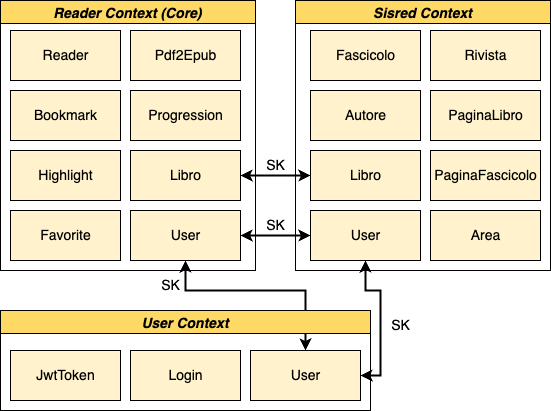
\includegraphics[width=0.75\textwidth]{img/ddd-context-map.png}
    \caption{Panoramica globale dei contesti del progetto e delle relazioni che intercorrono tra di essi}
    \label{context-map-png}
\end{figure}

Tra i contesti definiti esistono delle relazioni di tipo \textit{Shared Kernel}~\cite{evans_domain-driven_2004} (SK) con l'obiettivo di evitare duplicazioni e semplificare l'integrazione.
Relazioni di questo tipo consistono nella condivisione di un sottoinsieme del dominio modellato, 
che corrisponde tipicamente al dominio core. 
Un esempio di relazione SK è l'utilizzo di codice o schemi DB condivisi\footnote{\href{https://github.com/ddd-crew/context-mapping}{https://github.com/ddd-crew/context-mapping}}. 

Per la modellazione del dominio si fa uso dei seguenti concetti~\cite{evans_domain-driven_2004}:

\begin{itemize}
    \item \textbf{Entity} - Oggetto definito dalla sua identità e non dai suoi attributi. Ogni libro è univoco, identificato da uno specifico codice, chiamato ISBN\footnote{International Standard Book Number}.
    
    \item \textbf{Value Object} - Al contrario delle entità, questi oggetti sono definiti dai loro attributi e non hanno un'identità concettuale ma servono a descrivere alcune caratteristiche di un oggetto. Un esempio è il segnalibro: ciò che è rilevante è la pagina del libro che esso referenzia e non la sua identità.
    
    \item \textbf{Aggregate} - Insieme di oggetti legati da un'entità padre chiamata \textit{Root} (radice di aggregazione). L'aggregato composto da \textit{Bookmark}, \textit{Highlight}, \textit{Progression}, \textit{Favorite} ha come radice l'entità \textit{Libro}.

    \begin{figure}[H]
        \centering
        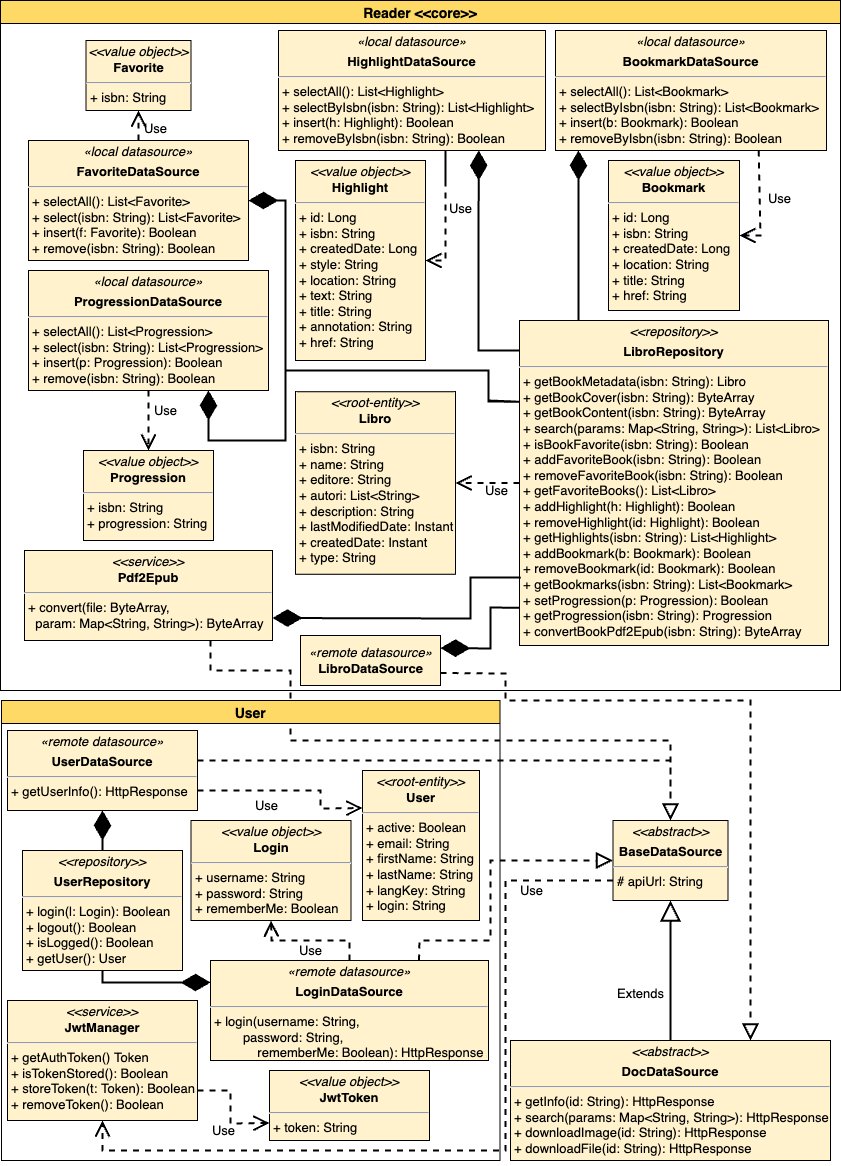
\includegraphics[width=1\textwidth]{img/class-uml-app.png}
        \caption{UML - Diagramma delle classi: Reader Core Domain e User Subdomain}
        \label{class-uml-app}
    \end{figure}

    \item \textbf{Service} - Operazione che non appartiene logicamente a nessun oggetto. In questo caso la conversione di formato non appartiene alla sola entità libro ma appartiene invece a qualsiasi documento che è possibile convertire.
    
    \item \textbf{Repository} - Oggetto per il recupero di altri oggetti di dominio e per la gestione del loro ciclo di vita. Le entità \textit{User} e \textit{Libro} sono esempi di oggetti di dominio che necessitano di un repository. Permette di disaccoppiare applicazione e domain design dalle specifiche tecnologie/strategie di persistenza come multipli database e datasource (locali e/o remoti).
\end{itemize}

\subsection{Progettazione UI/UX}
Successivamente alla modellazione del dominio e alla progettazione dell'architettura, 
le quali coinvolgono principalmente il modulo condiviso delle due applicazioni che si intende sviluppare grazie al framework KMM,
è necessario progettare l'interfaccia grafica e l'esperienza utente che dovrà essere implementata invece per le rispettive piattaforme Android e iOS. 
Considerando l'utilizzo tipico di un'applicazione con funzionalità simili a quella che deve essere realizzata,
possono essere adottati pattern di navigazione e visualizzazione dei contenuti diventati oramai standard de-facto nella progettazione della UI/UX e non solo per le applicazioni mobile\footnote{\href{https://xd.adobe.com/ideas/principles/app-design/}{https://xd.adobe.com/ideas/principles/app-design/}}.

Alcuni esempi di questi elementi utilizzati sono il menu laterale a scomparsa (schermata 4), 
l'icona "hamburger" per l'apertura del menu (schermata 3), 
l' elenco di documenti con scroll infinito verticale (schermata 2-5) e la barra di ricerca nella parte alta della schermata con icona "lente di ingrandimento" (schermata 2-5). 

Per ottenere la validazione dei mockup da parte del committente sono state necessarie due iterazioni del processo di progettazione UX/UI.
L'interfaccia utente desiderata deve infatti soddisfare alcuni vincoli caratteristici del brand Maggioli, 
come ad esempio l' utilizzo del colore blu \#00379E come colore primario, 
l'utilizzo del font Karla\footnote{\href{https://github.com/googlefonts/karla}{https://github.com/googlefonts/karla}} e la presenza del logo Maggioli. 
Le schermate necessarie per la realizzazione dell'applicazione sono:

\begin{itemize}
    \item \textbf{Reader} - Responsabile della visualizzazione del contenuto digitale in formato EPUB.
    
    \item \textbf{Login} - Schermata iniziale responsabile dell'autenticazione dell'utente.
    
    \item \textbf{Home} - Schermata principale responsabile alla visualizzazione dei contenuti digitali a cui l'utente è autorizzato ad accedere.
    
    \item \textbf{Preferiti} - Responsabile alla visualizzazione dei contenuti digitali preferiti dall'utente.
    
    \item \textbf{Impostazioni} - Responsabile alla visualizzazione e modifica delle impostazioni.
    
    \item \textbf{About} - Responsabile alla visualizzazione di informazioni generali come versione dell'applicazione, autore e copyright.
\end{itemize}

\begin{figure}[H]
    \centering
    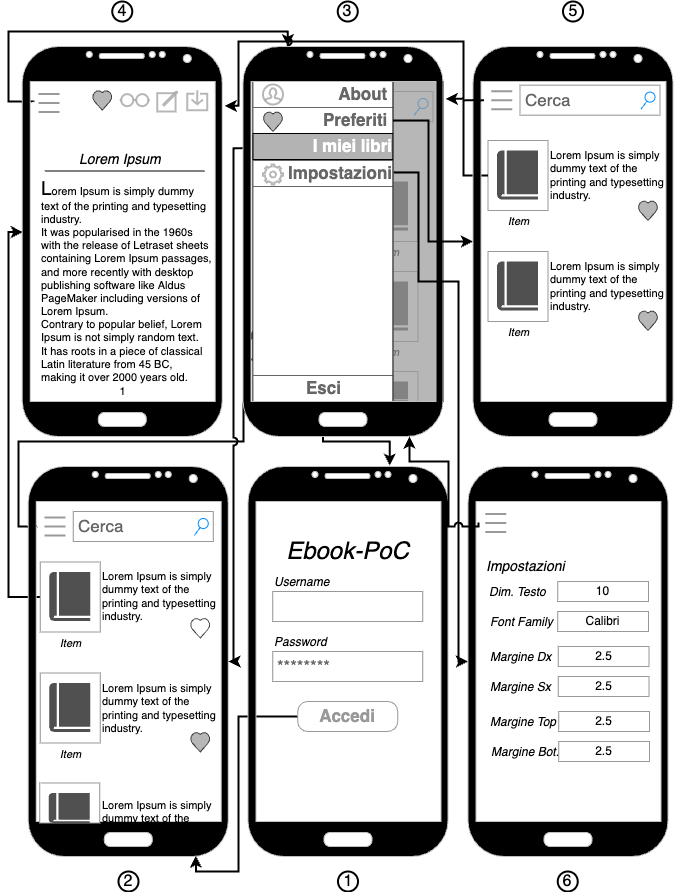
\includegraphics[width=1\textwidth]{img/mockup-uiux-1.png}
    \caption{Alcuni dei mockup realizzati per la progettazione e la validazione della UX/UI (prima iterazione)}
\end{figure}

\begin{figure}[H]
    \centering
    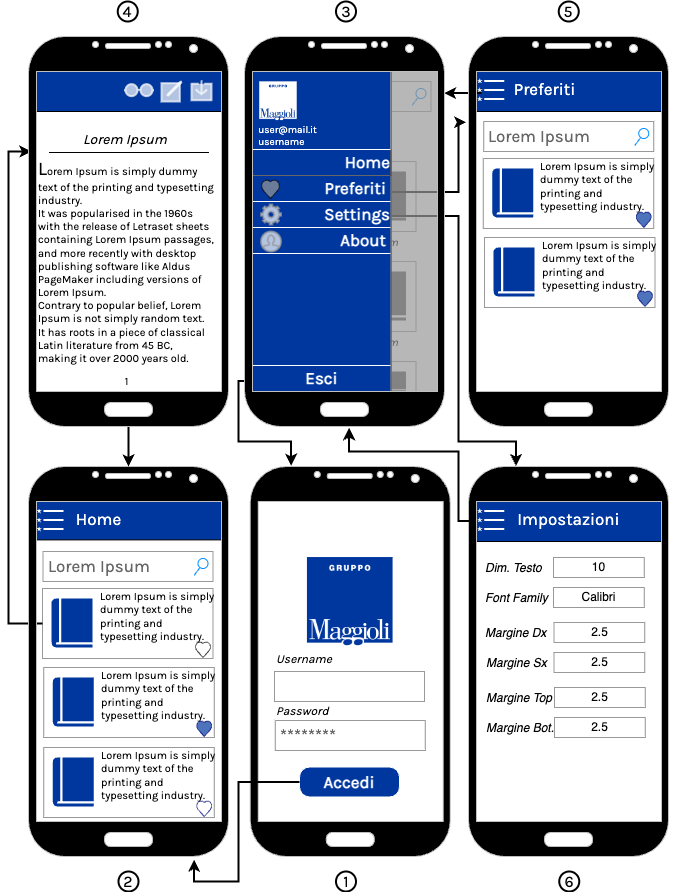
\includegraphics[width=1\textwidth]{img/mockup-uiux-2.png}
    \caption{Modifiche apportate ai mockup per ottenere la validazione della UX/UI (seconda iterazione)}
\end{figure}

\subsection{Architettura}
Lo scopo di un'applicazione multipiattaforma è la condivisione della sola logica applicativa come mostrato nella struttura di un'applicazione KMM (fig. \ref{stackKMM}). 
L'architettura in grado di supportare efficacemente questo concetto è conosciuta come \textit{Clean Architecture}~\cite{martin2017architecture} ed è composta da tre strati. 
Il primo strato (\textit{Data Layer}) consiste negli aggregati di dominio sopra descritti ed è responsabile per il recupero e il mantenimento dei dati su differenti sorgenti. 
Il secondo strato (\textit{Domain Layer}) facilità la comunicazione tra i differenti repository:
qui si trovano tutti i casi d'uso del sistema che gestiscono il flusso dei dati provenienti o diretti verso il primo strato. 
Il terzo ed ultimo strato (\textit{View Layer}) si occupa dell'interfaccia grafica mostrando i dati e gestendo gli eventi provenienti dall'utente o dal sistema.

\begin{figure}[H]
    \centering
    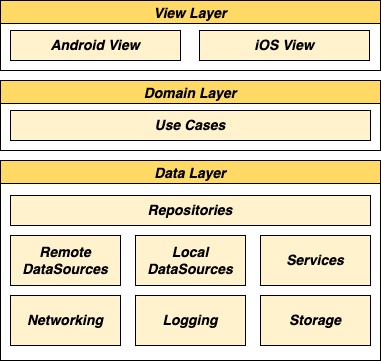
\includegraphics[width=0.55\textwidth]{img/clean-architecture.png}
    \caption{Clean Architecture in MaggioliEbook}
    \label{clean-arch-kmm-fig}
\end{figure}

\section{Sviluppo}
Tipicamente lo sviluppo effettivo di un'applicazione multiplatform con il framework KMM ha inizio con la creazione dello scheletro dell'applicazione tramite l'IDE Android Studio e il relativo plugin Gradle KMM, 
come indicato nel capitolo \ref{ch:app-multiplatform}.

La prima attività successiva alla creazione dello scheletro del progetto consiste nella ricerca delle librerie, 
ovvero le stesse dipendenze che sono gestite in modo automatico dal sistema d'automazione come descritto nel capitolo precedente. 
Considerando le funzionalità che devono essere implementate è necessario individuare tutte le librerie utili partendo da quelle core, 
come la visualizzazione e la modifica dei documenti, 
arrivando a quelle di utilità a supporto del modulo condiviso come networking e storage. 
Raggruppate per modulo di utilizzo, 
le librerie individuate e adottate sono:

\subsubsection*{Shared}
\begin{itemize} 
    \item \textbf{Ktor}\footnote{\href{https://github.com/ktorio/ktor}{https://github.com/ktorio/ktor}} - Framework asincrono per lo sviluppo di microservizi e applicazioni web, utilizzato per la parte di networking come client HTTP.
    
    \item \textbf{Kotlinx-Serialization} - Libreria multiplatform per la serializzazione dei dati.
    
    \item \textbf{Kotlinx-Datetime} - Libreria multiplatform per la gestione delle date e del tempo.
    
    \item \textbf{Kvault}\footnote{\href{https://github.com/Liftric/KVault}{https://github.com/Liftric/KVault}} - Libreria multiplatform per la persistenza dei dati sicura in formato chiave-valore. Tramite un'unica API si comporta come wrapper di \textit{Keychain}\footnote{\href{https://developer.apple.com/documentation/security/keychain\_services}{https://developer.apple.com/documentation/security/keychain\_services}}, nel caso iOS, e \textit{SharedPreferences}\footnote{\href{https://developer.android.com/reference/android/content/SharedPreferences}{https://developer.android.com/reference/android/content/SharedPreferences}} nel caso Android.
    
    \item \textbf{Koin}\footnote{\href{https://github.com/InsertKoinIO/koin}{https://github.com/InsertKoinIO/koin}} - Dependency Injection framework multiplatform.
    
    \item \textbf{Napier}\footnote{\href{https://github.com/AAkira/Napier}{https://github.com/AAkira/Napier}} - Logging framework multiplatform.
    
    \item \textbf{SqlDelight}\footnote{\href{https://github.com/cashapp/sqldelight}{https://github.com/cashapp/sqldelight}} - Libreria multiplatform per la persistenza dei dati tramite database relazionale locale.
\end{itemize}

\subsubsection*{Android}
\begin{itemize}
    \item \textbf{Readium} (\textit{Kotlin-toolkit})\footnote{\href{https://github.com/readium/kotlin-toolkit}{https://github.com/readium/kotlin-toolkit}} - Libreria per la manipolazione e la visualizzazione di pubblicazioni digitali. Implementazione specifica per la piattaforma Android. 
\end{itemize}

\subsubsection*{iOS}
\begin{itemize}
    \item \textbf{Readium} (\textit{Swift-toolkit})\footnote{\href{https://github.com/readium/swift-toolkit}{https://github.com/readium/swift-toolkit}} - Libreria per la manipolazione e la visualizzazione di pubblicazioni digitali. Implementazione specifica per la piattaforma iOS. 
\end{itemize}
    
\subsection{Readium}
La necessità di un tool open-source, 
robusto e performante per la manipolazione e la lettura di formati editoriali digitali è alla base del progetto Readium. 
Essa infatti consiste in un insieme di toolkit per diversi formati (come EPUB, audiolibri e libri image-based) e diverse piattaforme (Android, iOS, Desktop e Web).

L'architettura della libreria Readium è composta da tre moduli principali:

\begin{itemize}
    \item \textbf{Publication Server} - Fornisce le pubblicazioni tramite un server locale HTTPS.
    
    \item \textbf{Streamer} - Modulo composto dai seguenti due sottomoduli:
    \begin{itemize}
        \item \textbf{Parser} - Responsabile del parsing delle pubblicazioni e della loro esposizione utilizzando un modello in-memory.
        
        \item \textbf{Fetcher} - Si occupa di ottenere i contenuti delle pubblicazioni e della loro manipolazione (in particolare injection di CSS e Javascript nelle risorse HTML).
    \end{itemize}
    
    \item \textbf{Navigator} - Utile alla navigazione delle risorse di una pubblicazione secondo diverse strategie basate sulla natura della pubblicazione (ebook, audiolibri, ...). Interagisce con il modulo \textit{Streamer} per utilizzare il modello in-memory o per ottenere il manifesto JSON attraverso il modello condiviso (\textit{Shared}).
\end{itemize}

\begin{figure}[H]
    \centering
    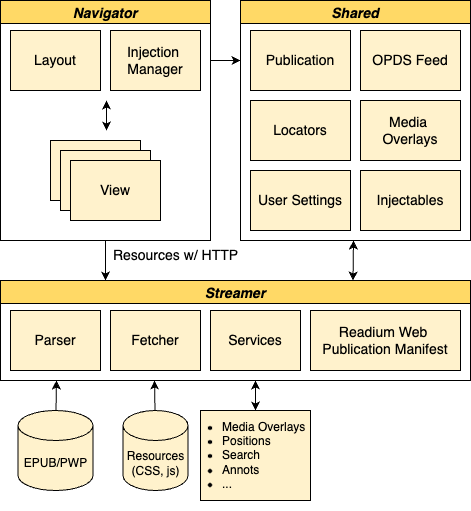
\includegraphics[width=0.65\textwidth]{img/readium-arch.png}
    \caption{Architettura libreria Readium}
    \label{readiumarch}
\end{figure}

\subsection{Modulo Shared}
Come anticipato nel capitolo \ref{ch:app-multiplatform} la parte condivisa di un'applicazione multipiattaforma racchiude tutta o una sottoparte della logica applicativa, 
compresi quindi anche aspetti ``infrastrutturali'' specifici della piattaforma target come ad esempio logging, persistenza dei dati e networking.

Gli elementi del dominio che sono stati aggiunti dal contesto core (fig. \ref{context-map-png}) devono essere persistiti sul dispositivo locale ed è necessario svolgere operazioni CRUD\footnote{Create-Read-Update-Delete} come su qualsiasi database, 
che sia locale o remoto. 
I relativi schemi per il database locale sono stati definiti utilizzando appositi file\footnote{\href{https://github.com/paganellif/DevOps-per-applicazioni-mobile-un-caso-di-studio-industriale/tree/6-sviluppo-applicazione-maggioliebook/maggioliEbookApp/shared/src/commonMain/sqldelight/it/filo/maggioliebook/db}{https://github.com/paganellif/DevOps-per-applicazioni-mobile-un-caso-di-studio-industriale/tree/6-sviluppo-applicazione-maggioliebook/maggioliEbookApp/shared/src/\\commonMain/sqldelight/it/filo/maggioliebook/db}}, 
uno per ciascuna delle entità che necessita di persistenza, 
che sono \textit{Highlight}, 
\textit{Favorite}, 
\textit{Progression} e \textit{Bookmark}.

Il seguente codice\footnote{\href{https://github.com/paganellif/DevOps-per-applicazioni-mobile-un-caso-di-studio-industriale/blob/6-sviluppo-applicazione-maggioliebook/maggioliEbookApp/shared/src/commonMain/sqldelight/it/filo/maggioliebook/db/Bookmark.sq}{https://github.com/paganellif/DevOps-per-applicazioni-mobile-un-caso-di-studio-industriale/blob/6-sviluppo-applicazione-maggioliebook/maggioliEbookApp/shared/src/\\commonMain/sqldelight/it/filo/maggioliebook/db/Bookmark.sq}} definisce,
tramite la sintassi SqlDelight,
lo schema \textit{Bookmark} e l'operazione associata di selezione tramite ISBN:

\begin{listing}[H]
    \inputminted{sql}{code/bookmark-sqldelight.sq}
    \caption{Esempio di definizione schema \textit{Bookmark} tramite sintassi SqlDelight}
\end{listing}

Tramite il task \textit{generateSqlDelightInterface} fornito dal plugin gradle SqlDelight è possibile generare automaticamente l'interfaccia padre \textit{MaggioliEbookDB} e le relative implementazioni. 
Nel caso dello schema sopra indicato si ottiene il seguente codice\footnote{\href{https://github.com/paganellif/DevOps-per-applicazioni-mobile-un-caso-di-studio-industriale/blob/6-sviluppo-applicazione-maggioliebook/maggioliEbookApp/shared/build/generated/sqldelight/code/MaggioliEbookDB/commonMain/it/filo/maggioliebook/db/BookmarkQueries.kt}{https://github.com/paganellif/DevOps-per-applicazioni-mobile-un-caso-di-studio-industriale/blob/6-sviluppo-applicazione-maggioliebook/maggioliEbookApp/shared/build/generated/\\sqldelight/code/MaggioliEbookDB/commonMain/it/filo/maggioliebook/db/BookmarkQueries.kt}} Kotlin:

\begin{listing}[H]
    \inputminted{kotlin}{code/bookmark-sqldelight.kt}
    \caption{Codice Kotlin autogenerato per lo schema \textit{Bookmark} tramite SqlDelight}
\end{listing}

\begin{figure}[H]
    \centering
    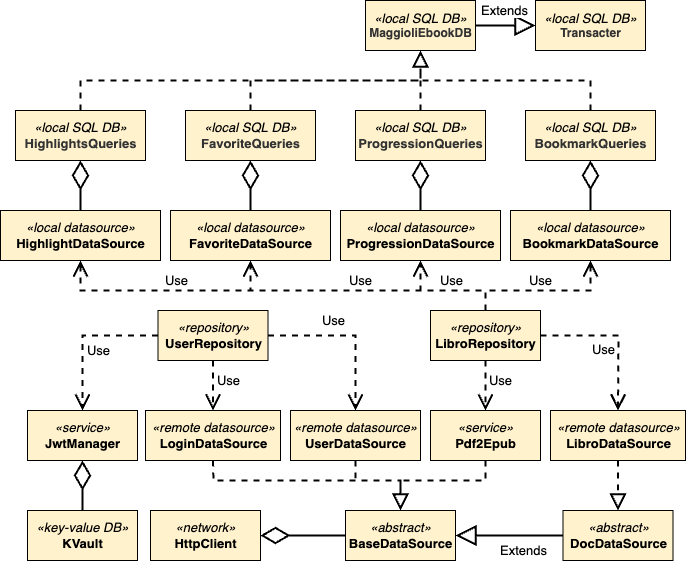
\includegraphics[width=0.95\textwidth]{img/uml-network-db.png}
    \caption{UML - Diagramma delle classi: Implementazioni data source (persistenza dati e networking)}
\end{figure}

Tipicamente le librerie per applicazioni sviluppate con Kotlin Multiplatform possono essere utilizzate direttamente dal codice condiviso,
come ad esempio KVault, 
lasciando al compilatore Kotlin il compito di scegliere la giusta implementazione per la piattaforma target durante la fase di compilazione. 
In altri casi è necessario invece utilizzare il meccanismo \textit{expect/actual} (discusso nel capitolo \ref{ch:app-multiplatform}) per definire il comportamento atteso e fornire un'implementazione specifica per la piattaforma target.

Tale meccanismo è stato utilizzato nello sviluppo dell'applicazione per poter effettuare dependency injection tramite la libreria Koin dei componenti riguardanti la persistenza dei dati (Kvault e SqlDelight) e l'esecuzione asincrona (CoroutineDispatcher). 
Ogni dipendenza che deve essere iniettata viene inserita all'interno di uno o più moduli,
i quali vengono utilizzati da Koin per inizializzare tutto il contesto applicativo, 
come nel seguente esempio\footnote{\href{https://github.com/paganellif/DevOps-per-applicazioni-mobile-un-caso-di-studio-industriale/blob/6-sviluppo-applicazione-maggioliebook/maggioliEbookApp/shared/src/commonMain/kotlin/it/filo/maggioliebook/di/KoinModule.kt}{https://github.com/paganellif/DevOps-per-applicazioni-mobile-un-caso-di-studio-industriale/blob/6-sviluppo-applicazione-maggioliebook/maggioliEbookApp/shared/src/commonMain/\\kotlin/it/filo/maggioliebook/di/KoinModule.kt}} del caso di studio realizzato. 

Le dipendenze possono essere principalmente di due tipi:

\begin{itemize}
    \item \textbf{Factory} - Ogni volta che la dipendenza viene iniettata ne viene creata una nuova istanza (paragonabile al design pattern Factory Method~\cite{gamma1994design}).
    
    \item \textbf{Single} - In tutto il contesto applicativo esiste una sola istanza della dipendenza iniettata (paragonabile al design pattern Singleton~\cite{gamma1994design}).
\end{itemize}

\begin{figure}[H]
    \centering
    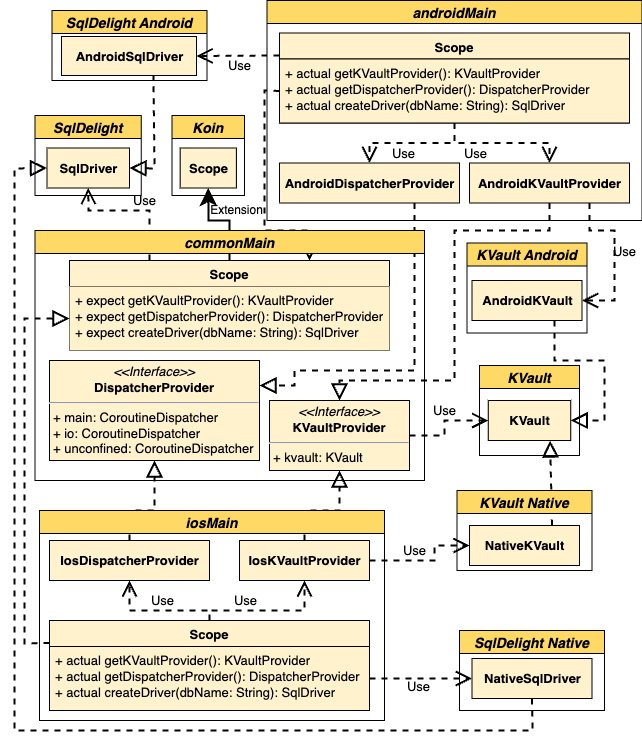
\includegraphics[width=0.95\textwidth]{img/expect-actual-shared.png}
    \caption{Strategia \textit{Expect/Actual} adottata per l'implementazione dei servizi infrastrutturali specifici delle piattaforme (persistenza e concorrenza) sfruttando la tecnica \textit{dependency injection}}
\end{figure}

\begin{listing}[H]
    \inputminted{kotlin}{code/shared-di-koin.kt}
    \caption{Configurazione Dependency Injection: definizione dei moduli Koin e inizializzazione del contesto applicativo}
\end{listing}

\subsection{Applicazione Android}
Completato lo sviluppo della logica applicativa condivisa e quindi degli strati \textit{Domain} e \textit{Data} (fig. \ref{clean-arch-kmm-fig}) dell'architettura, 
è possibile iniziare lo sviluppo dello strato \textit{View}. 
In questa fase si realizza la vera e propria applicazione Android,
sfruttando il toolkit Kotlin della libreria Readium per la funzionalità core di lettura dei contenuti digitali.

\subsubsection*{Single-Activity Architecture}
L'architettura scelta per l'implementazione dell'applicazione Android\footnote{\href{https://github.com/paganellif/DevOps-per-applicazioni-mobile-un-caso-di-studio-industriale/tree/6-sviluppo-applicazione-maggioliebook/maggioliEbookApp/androidMaggioliEbookApp/src/main/java/it/filo/maggioliebook/android}{https://github.com/paganellif/DevOps-per-applicazioni-mobile-un-caso-di-studio-industriale/tree/6-sviluppo-applicazione-maggioliebook/maggioliEbookApp/androidMaggioliEbookApp/\\src/main/java/it/filo/maggioliebook/android}} è basata su sole due activity:

\begin{itemize}
    \item \textbf{MainActivity} - Unica activity principale dell'applicazione.
    
    \item \textbf{ReaderActivity} - Activity secondaria, utilizzata sia per l'interazione che la gestione del lettore delle pubblicazioni digitali.
\end{itemize}

Questa tipologia di architettura permette di avere una singola activity che svolge la funzione di contenitore per tutti i fragment che rappresentano le varie schermate, 
definite in fase di progettazione della UI/UX, 
in cui l'utente può navigare.

\begin{figure}[H]
    \centering
    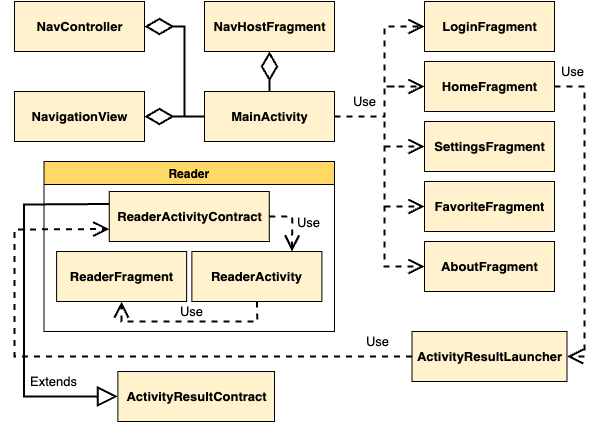
\includegraphics[width=0.77\textwidth]{img/android-arch.png}
    \caption{Architettura Single-Activity adottata per l'applicazione Android}
    \label{android-arch-png}
\end{figure}

La navigazione all'interno dell'applicazione è gestita tramite la combinazione dei seguenti componenti:

\begin{itemize}
    \item \textbf{NavController} - Componente necessario per la gestione delle transizioni da un fragment all'altro. Quando inizializzato, richiede la presenza di un grafo di navigazione tra le risorse XML: tale grafo contiene tutti i fragment che possono essere visualizzati e le possibili transizioni tra di essi.
    
    \item \textbf{NavHostFragment} - Rappresenta il contenitore del fragment in cui ci si trova. Ogni transizione nel grafo corrisponde alla sostituzione del fragment visualizzato con quello di destinazione (sempre che la transizione sia ammessa dal grafo).
    
    \item \textbf{NavigationView} - Permette la visualizzazione del menu dove si trovano i possibili fragment raggiungibili da quello in cui l'utente si trova attualmente. Nel caso dell'applicazione sviluppata, in questo componente si trova il menu laterale con tutte le schermate indicate in fase di progettazione (\textit{Home}, \textit{Settings}, \textit{About} e \textit{Preferiti}).
\end{itemize}

Come mostrato nella seguente figura (fig. \ref{android-nav-graph-png}), 
la schermata principale (\textit{Home}) rappresenta la destinazione iniziale del grafo, 
ovvero la prima schermata che viene visualizzata dall'applicazione. D
a questa schermata è poi possibile effettuare transizioni verso altre schermate sfruttando il meccanismo chiamato \textit{navigazione condizionale}\footnote{\href{https://developer.android.com/guide/navigation/navigation-conditional}{https://developer.android.com/guide/navigation/navigation-conditional}}. 
Prima di creare la vista del fragment viene effettuato un controllo sull'autenticazione dell'utente: 
se l'utente non è autenticato viene effettuata una transizione al fragment \textit{Login} per permettere all'utente di autenticarsi e procedere all'utilizzo dell'applicazione. 
E' fondamentale in questo scenario ripulire lo stack di navigazione per evitare che l'utente possa ``tornare indietro'' alla schermata precedente, 
ovvero la schermata principale, 
senza effettuare l'autenticazione.

\begin{figure}[H]
    \centering
    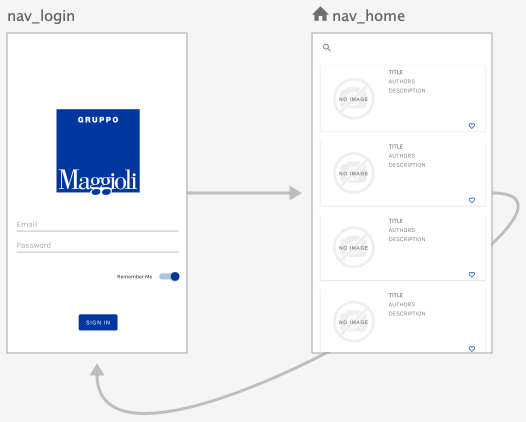
\includegraphics[width=0.62\textwidth]{img/android-nav-graph.png}
    \caption{Sottoparte del navigation graph dell'applicazione, renderizzato automaticamente tramite l'IDE Android Studio}
    \label{android-nav-graph-png}
\end{figure}

\subsubsection*{Paging}
\label{pagingsec}
Un altro aspetto importante dell'architettura è il meccanismo utilizzato sia dalla schermata principale che da quella dei preferiti per mostrare i dati all'utente.
Il backend utilizzato fornisce i dati tramite paginazione: 
in questo modo è possibile indicare in una richiesta la dimensione delle pagine, 
ovvero quanti elementi devono essere restituiti al massimo in una pagina, 
e la pagina desiderata. 
Per poter caricare tali dati dinamicamente in una \textit{RecyclerView}\footnote{\href{https://developer.android.com/reference/kotlin/androidx/recyclerview/widget/RecyclerView}{https://developer.android.com/reference/kotlin/androidx/recyclerview/widget/RecyclerView}}, in modo da permettere all'utente di effettuare lo scroll "infinito", è stata utilizzata\footnote{\href{https://github.com/paganellif/DevOps-per-applicazioni-mobile-un-caso-di-studio-industriale/blob/6-sviluppo-applicazione-maggioliebook/maggioliEbookApp/androidMaggioliEbookApp/src/main/java/it/filo/maggioliebook/android/home/LibroPagingSource.kt}{https://github.com/paganellif/DevOps-per-applicazioni-mobile-un-caso-di-studio-industriale/blob/6-sviluppo-applicazione-maggioliebook/maggioliEbookApp/androidMaggioliEbookApp/\\src/main/java/it/filo/maggioliebook/android/home/LibroPagingSource.kt}} la libreria \textit{Paging}\footnote{\href{https://developer.android.com/topic/libraries/architecture/paging/v3-overview}{https://developer.android.com/topic/libraries/architecture/paging/v3-overview}} fornita nativamente dall'SDK Android.

I componenti fondamentali della libreria \textit{Paging} sono:

\begin{itemize}
    \item \textbf{Pager} - Punto d'ingresso principale della libreria con il compito di ottenere nuovi dati quando necessario, ovvero quando l'utente ha raggiunto nella schermata uno specifico punto. Richiede la configurazione di alcuni parametri come la dimensione della pagina, la pagina iniziale e la direzione della paginazione. 
    
    \item \textbf{PagingSource} - Sorgente dei dati paginati. Componente interrogato dal \textit{Pager} ogni volta che sono necessari nuovi dati.
    
    \item \textbf{PagingDataAdapter} - Componente fondamentale per la rappresentazione di dati paginati in una \textit{RecyclerView}.
\end{itemize}

\begin{figure}[H]
    \centering
    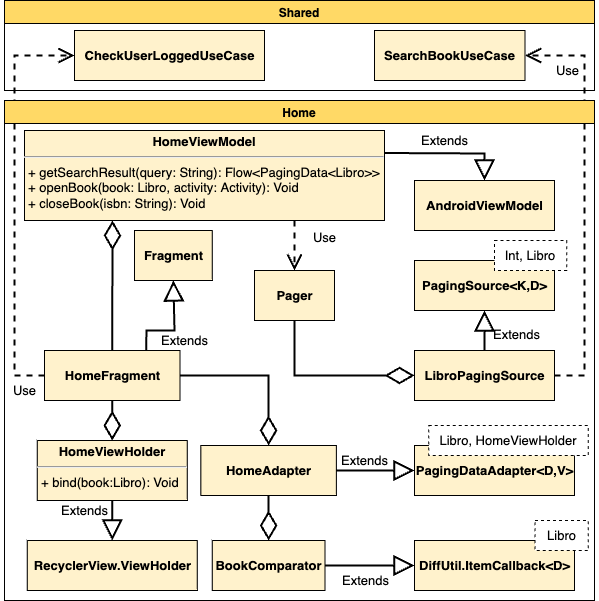
\includegraphics[width=0.8\textwidth]{img/android-viewmodel.png}
    \caption{UML - Diagramma delle classi: Paginazione dati nella schermata principale}
    \label{android-viewmodel-png}
\end{figure}

\subsubsection*{Reader}
Il lettore dei documenti digitali in formato EPUB rappresenta la funzionalità core dell'applicazione sviluppata. 
Nel caso dell'interfaccia grafica Android,
il lettore riceve il contenuto da visualizzare del documento selezionato dall'utente e lo mostra in un fragment basato sul componente \textit{Navigator} (fig. \ref{readiumarch}). 
Questo componente della libreria Readium fornisce tutte le funzionalità necessarie per gestire la navigazione dei documenti e gli eventi relativi al comportamento dell'utente come scorrimento pagine e selezione testo. 
I principali componenti sviluppati\footnote{\href{https://github.com/paganellif/DevOps-per-applicazioni-mobile-un-caso-di-studio-industriale/tree/6-sviluppo-applicazione-maggioliebook/maggioliEbookApp/androidMaggioliEbookApp/src/main/java/it/filo/maggioliebook/android/reader}{https://github.com/paganellif/DevOps-per-applicazioni-mobile-un-caso-di-studio-industriale/tree/6-sviluppo-applicazione-maggioliebook/maggioliEbookApp/androidMaggioliEbookApp/\\src/main/java/it/filo/maggioliebook/android/reader}} per le funzionalità del reader sono:

\begin{itemize}
    \item \textbf{ReaderActivity} - Unica activity presente nell'applicazione oltre a quella principale, utilizzata sia per l’interazione che per la gestione del lettore di contenuti digitali.

    \begin{figure}[H]
        \centering
        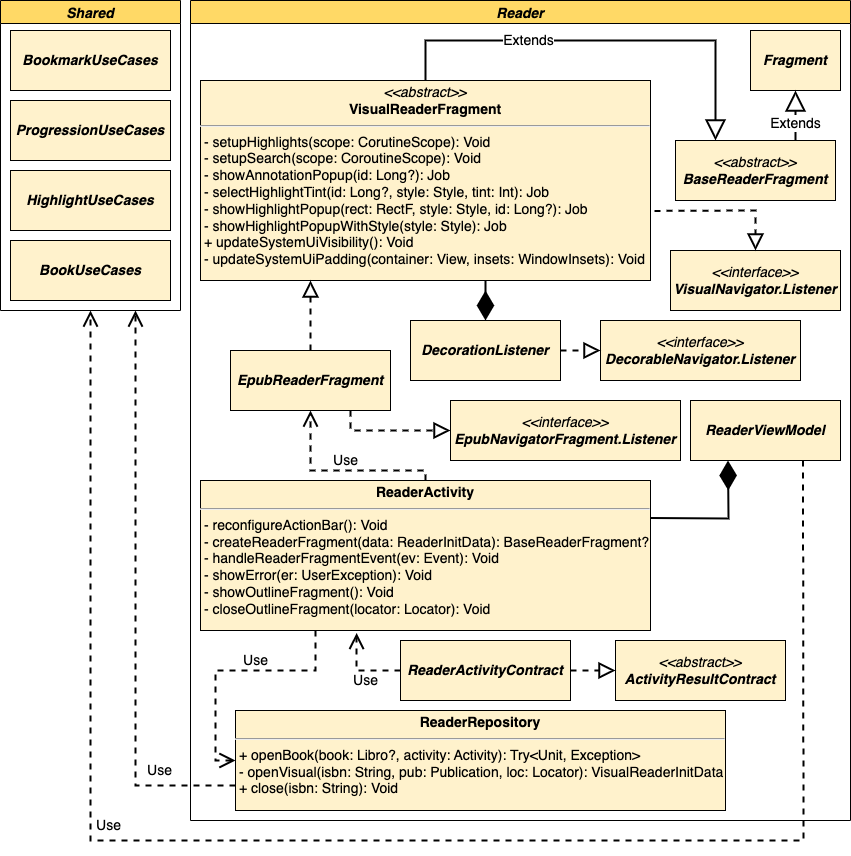
\includegraphics[width=1\textwidth]{img/reader-uml.png}
        \caption{UML - Diagramma delle classi: Reader}
        \label{reader-uml}
    \end{figure}
    
    \item \textbf{EpubReaderFragment} - Componente che si occupa effettivamente di mostrare il contenuto del documento all'utente.
    
    \item \textbf{DecorationListener} - Permette la gestione grafica delle annotazioni come evidenziazioni e sottolineature, le quali sono aggiunte alla vista del fragment tramite l'utilizzo di Jetpack Compose.
\end{itemize}

\newpage
\subsubsection*{Screenshot}
\begin{multicols}{3}
            \begin{figure}[H]
                \centering
                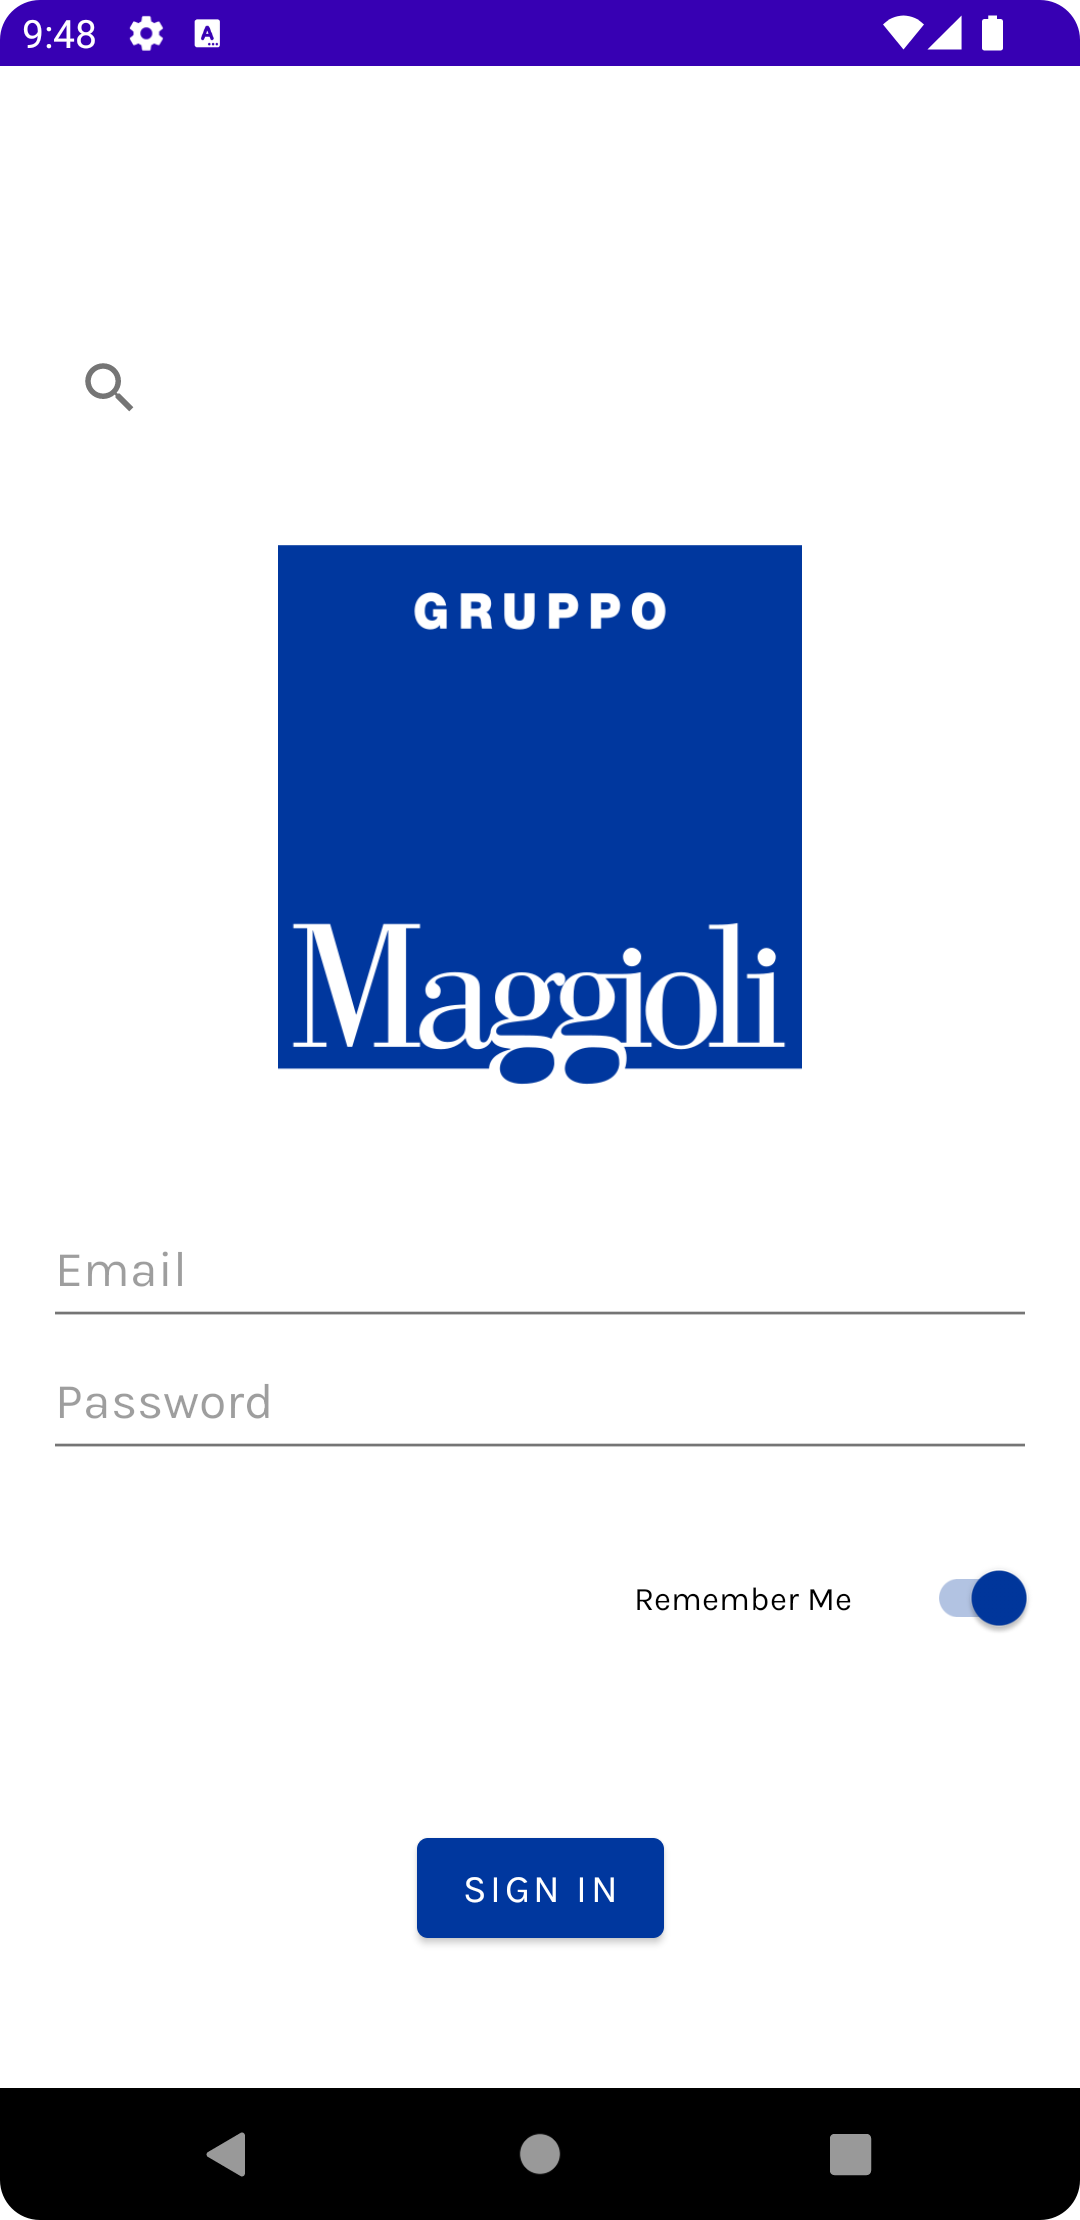
\includegraphics[width=0.29\textwidth]{img/login.png}
                \caption{Login}
                \label{login-android}
            \end{figure}

            \begin{figure}[H]
                \centering
                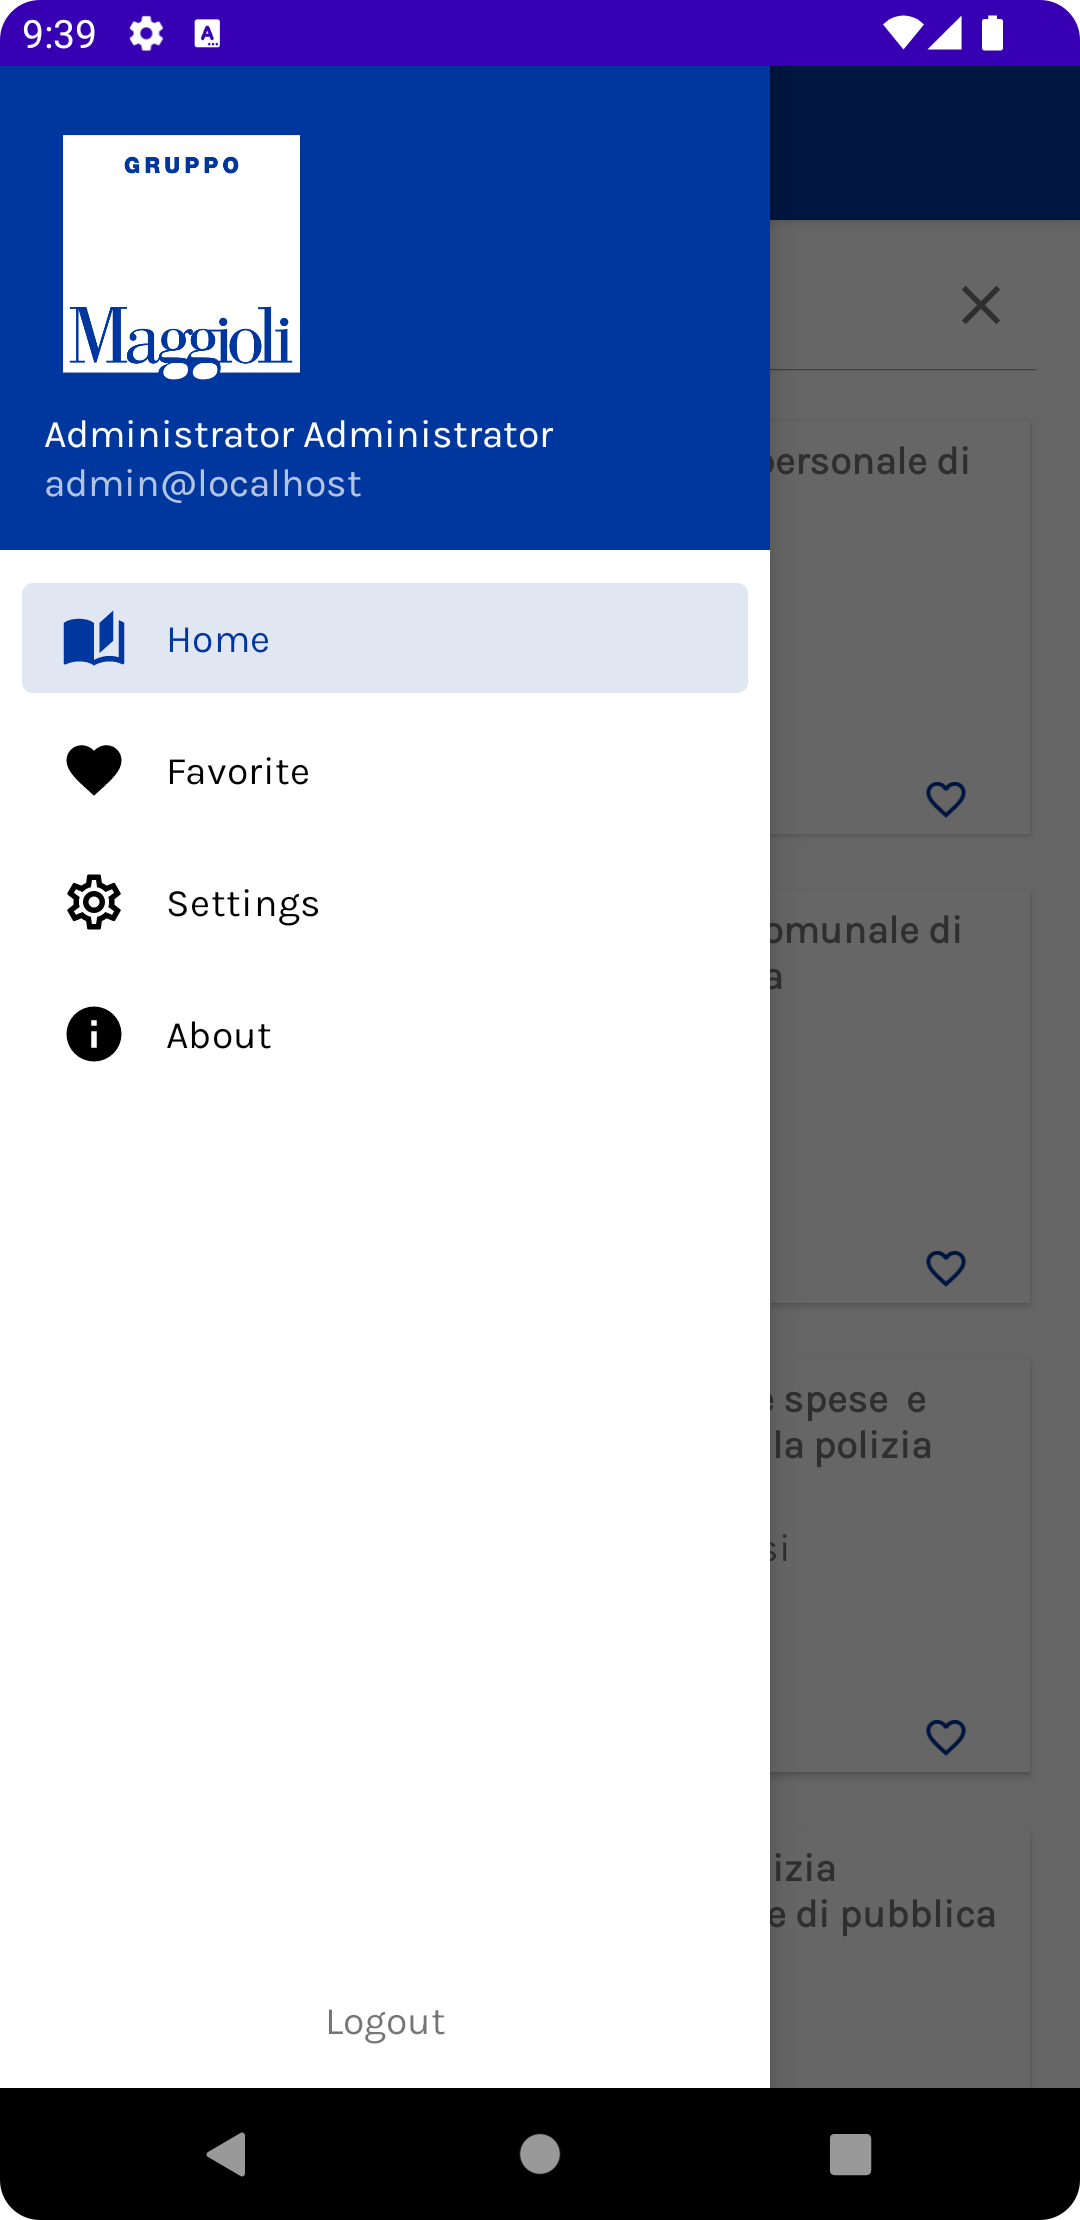
\includegraphics[width=0.29\textwidth]{img/sidenav.png}
                \caption{Menu laterale - Sidenav}
                \label{sidenav-android}
            \end{figure}
            
            \begin{figure}[H]
                \centering
                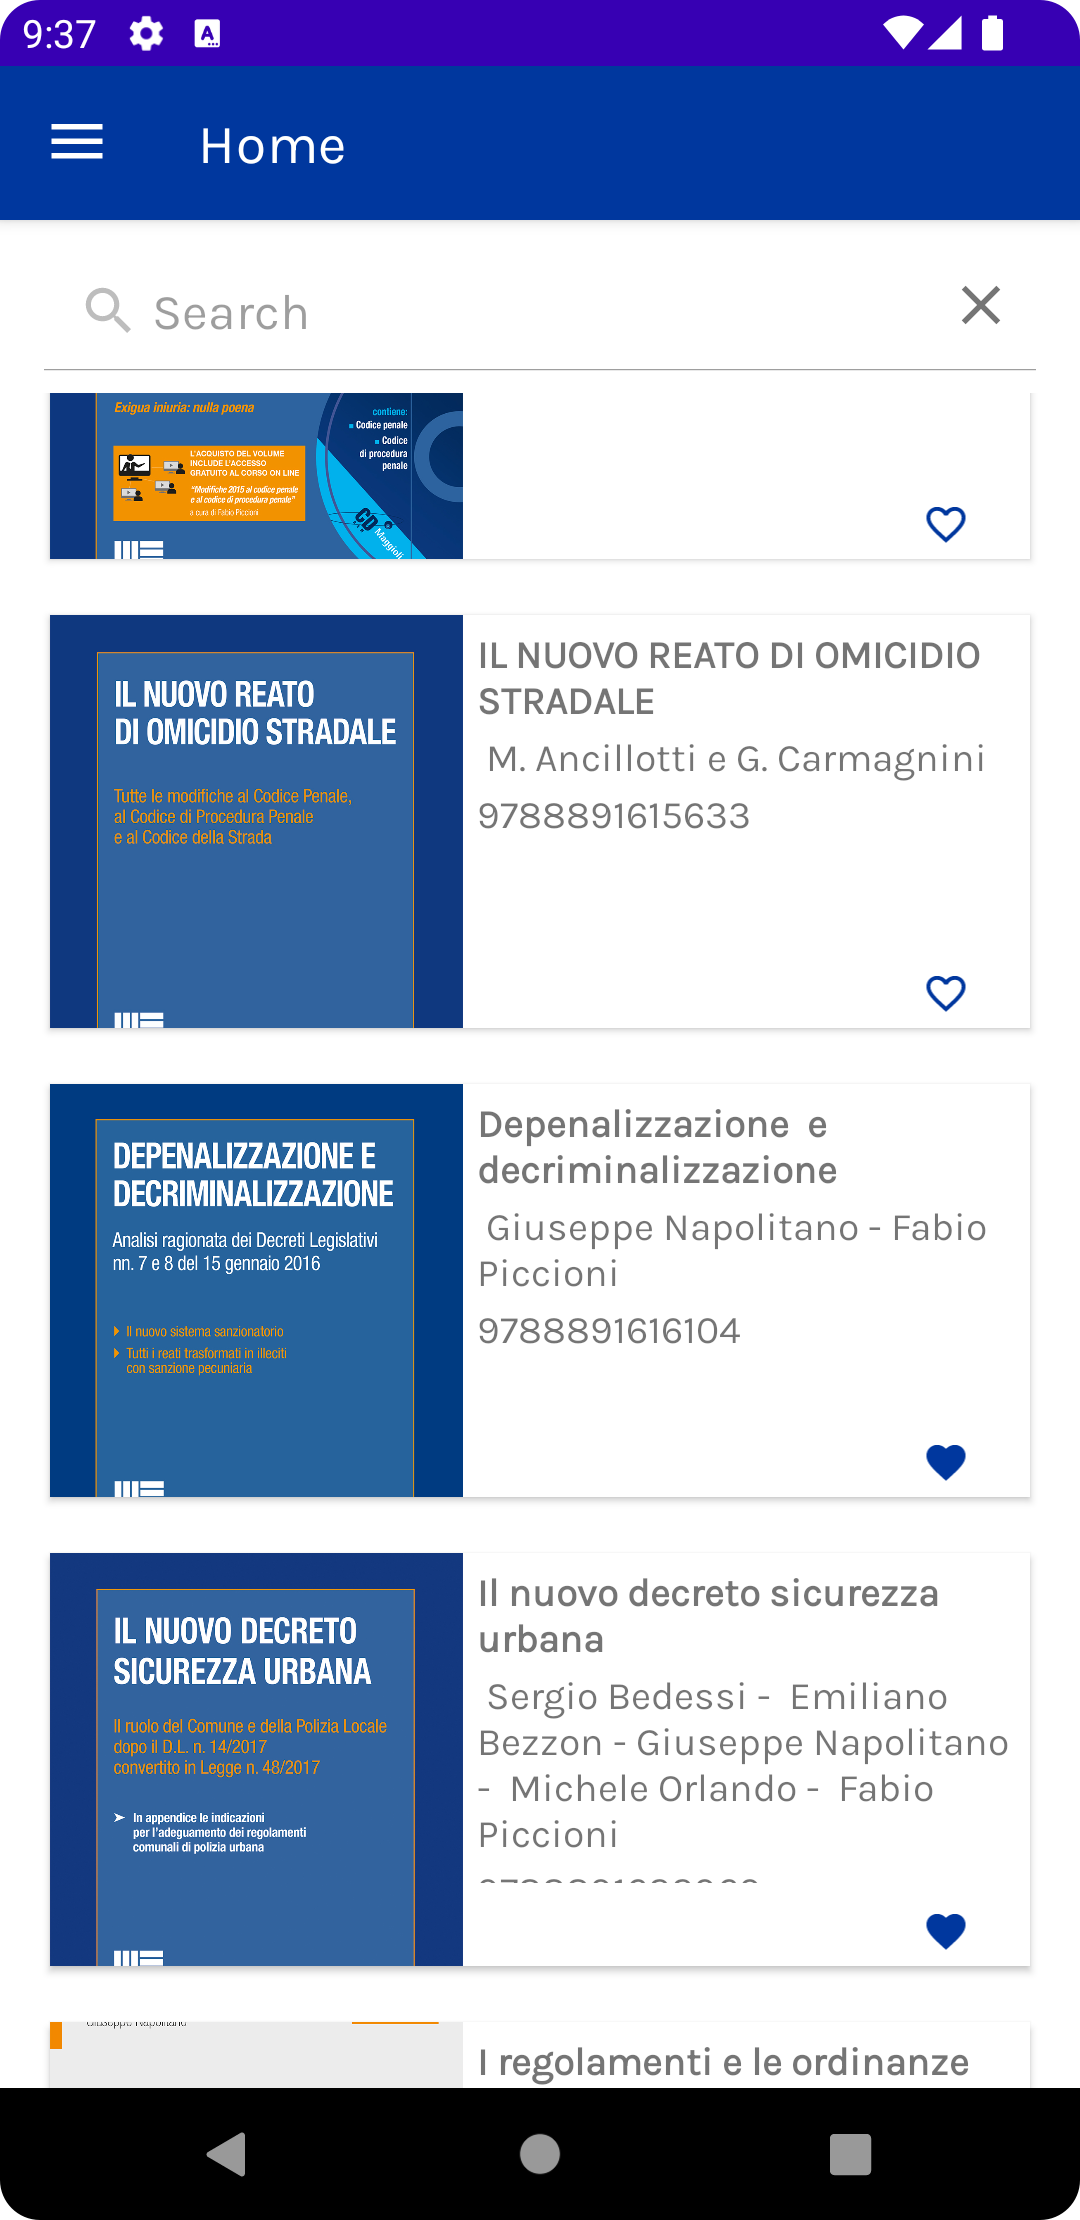
\includegraphics[width=0.29\textwidth]{img/home.png}
                \caption{Schermata home principale}
                \label{home-android}
            \end{figure}
            
            \begin{figure}[H]
                \centering
                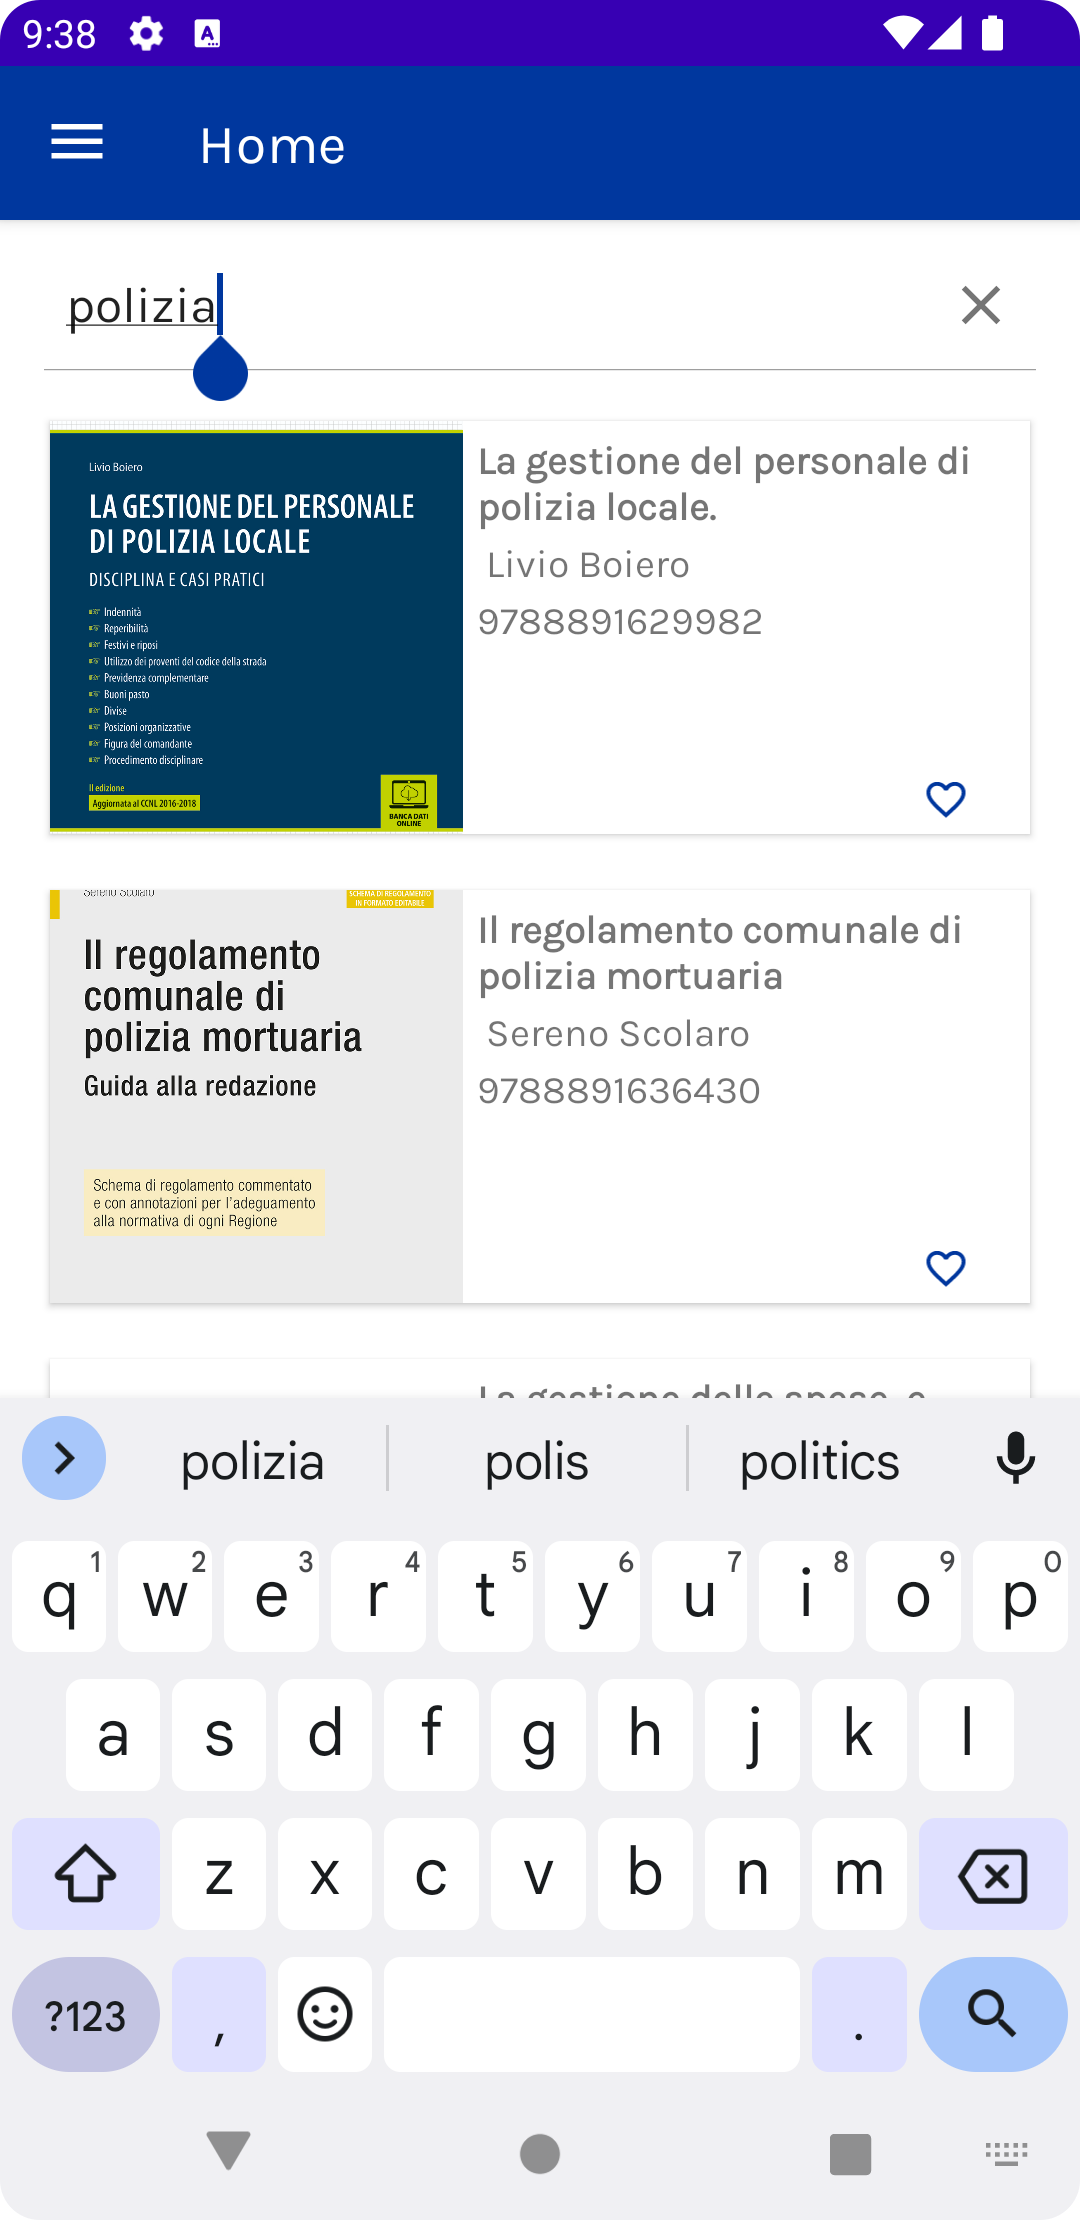
\includegraphics[width=0.29\textwidth]{img/ricerca.png}
                \caption{Esempio di ricerca}
                \label{ricerca-android}
            \end{figure}

            \begin{figure}[H]
                \centering
                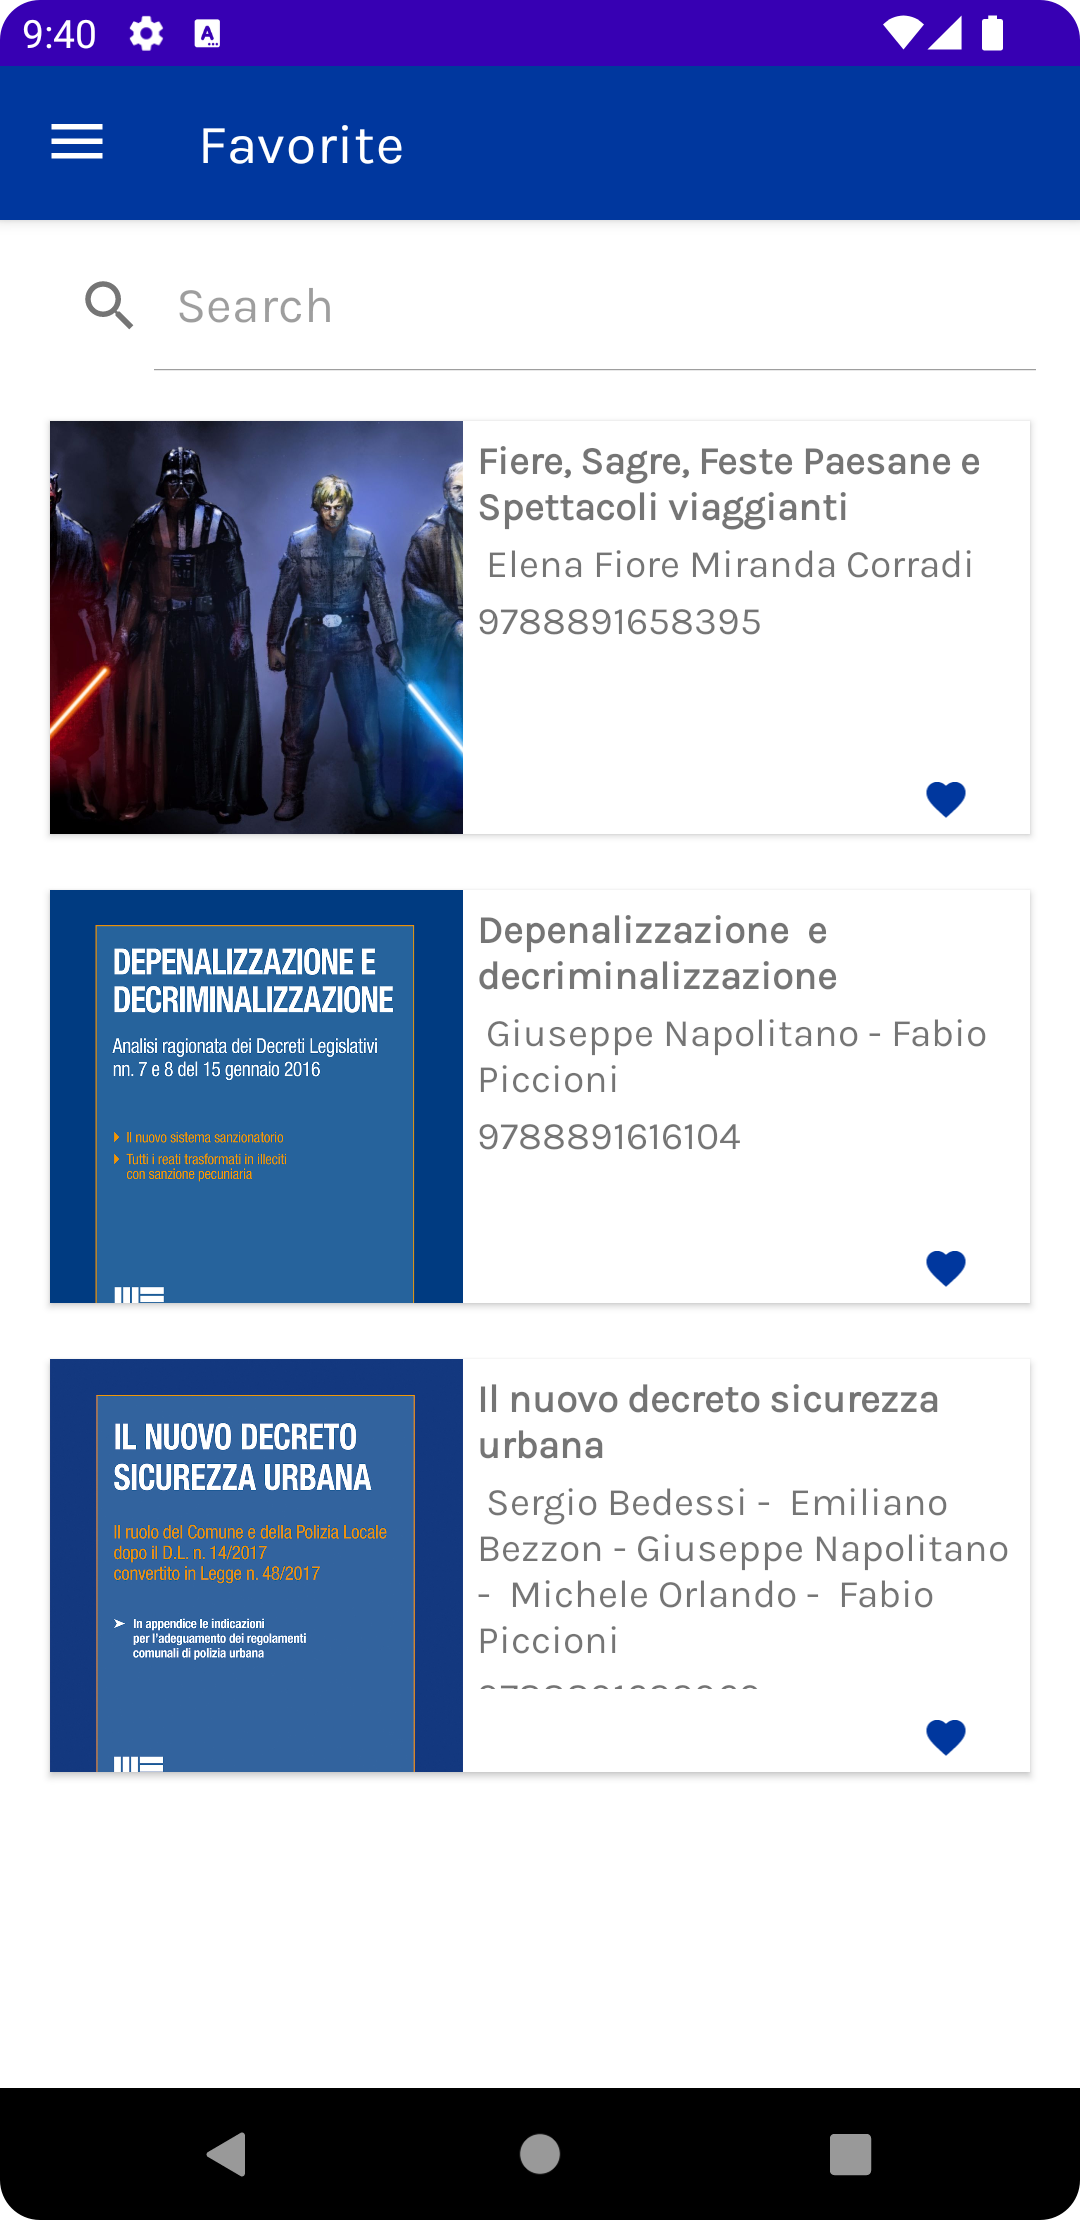
\includegraphics[width=0.29\textwidth]{img/preferiti.png}
                \caption{Preferiti}
                \label{preferiti-android}
            \end{figure}

            \begin{figure}[H]
                \centering
                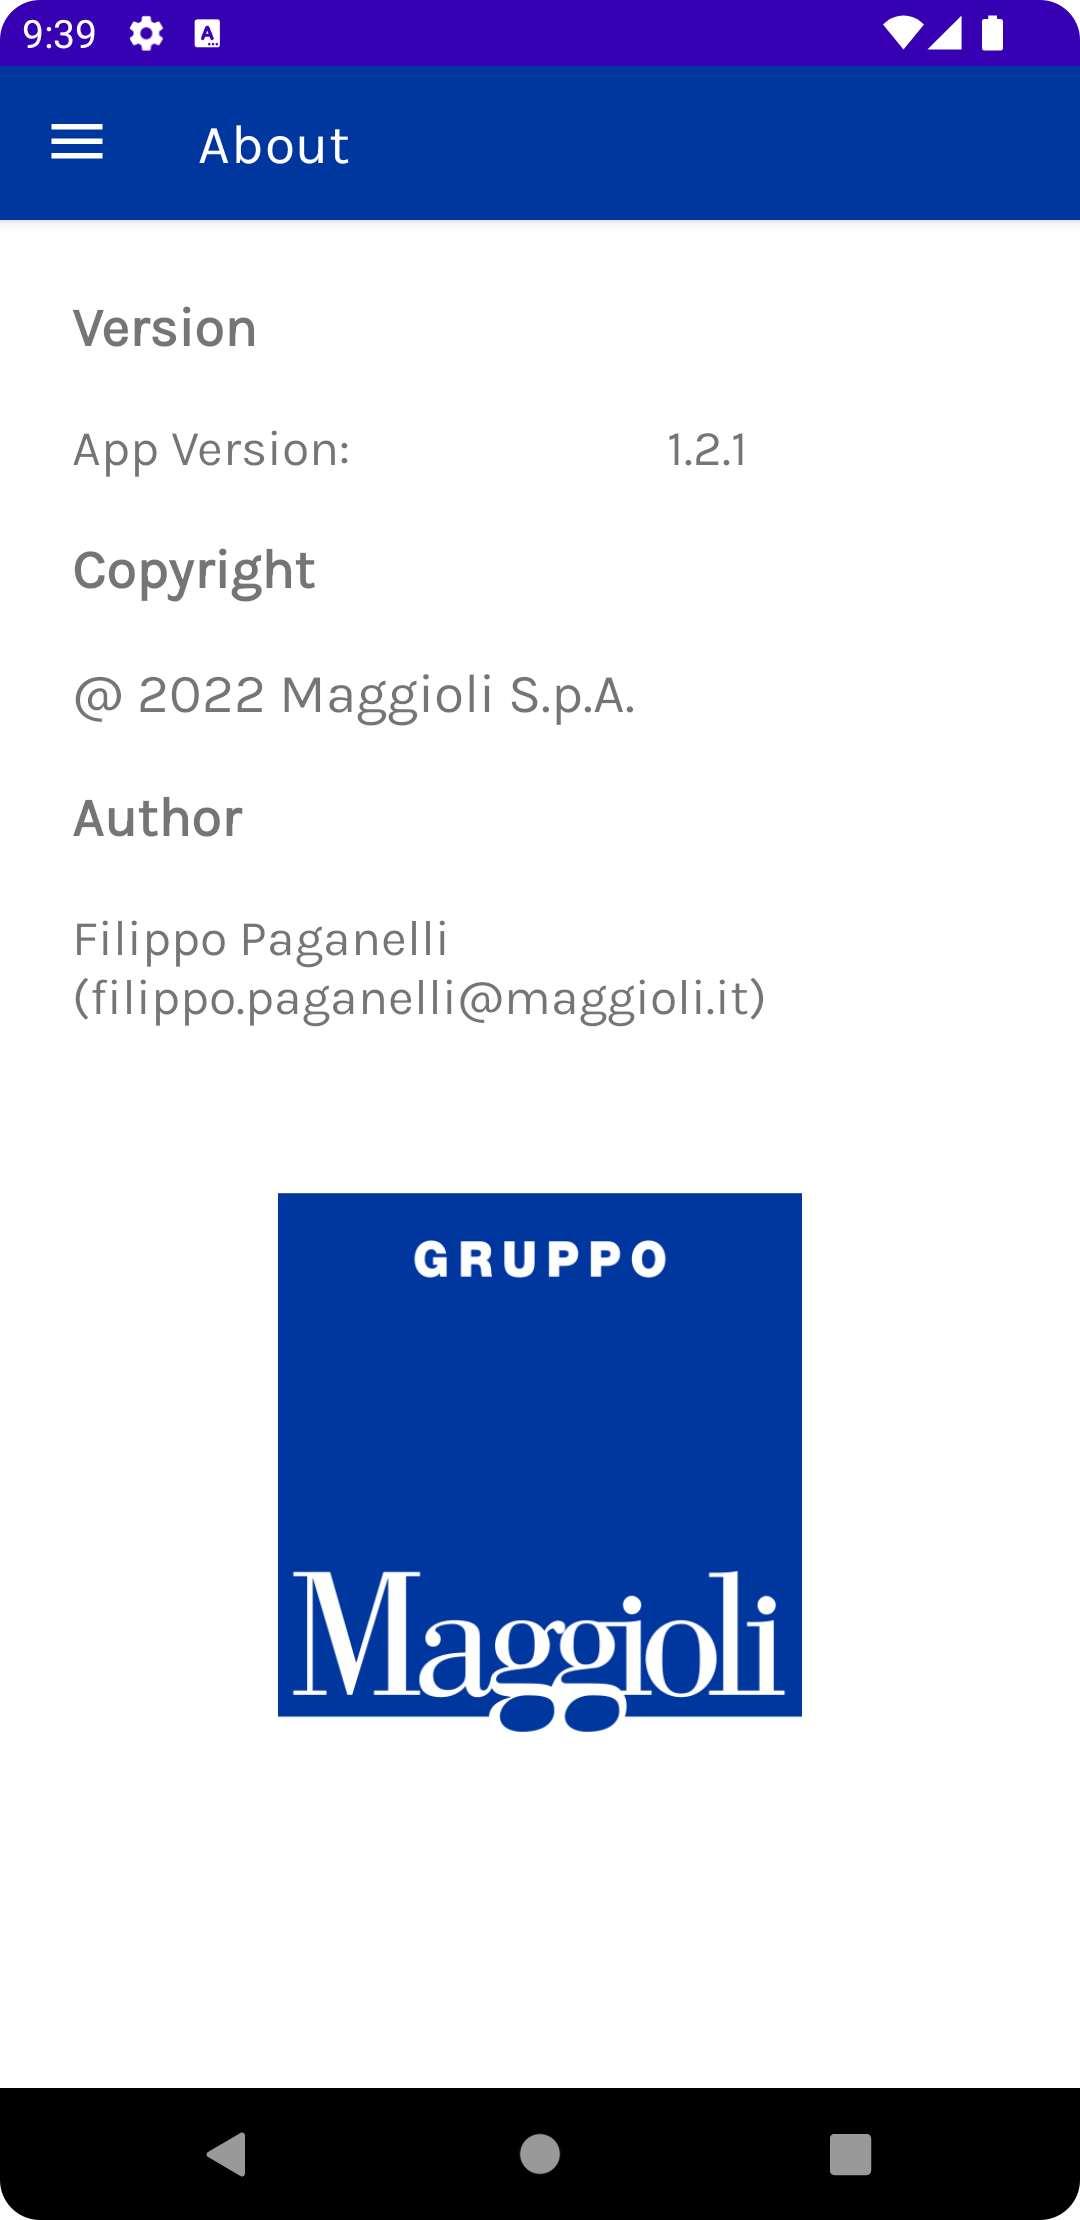
\includegraphics[width=0.29\textwidth]{img/about.png}
                \caption{Info generali (About)}
                \label{about-android}
            \end{figure}

            \begin{figure}[H]
                \centering
                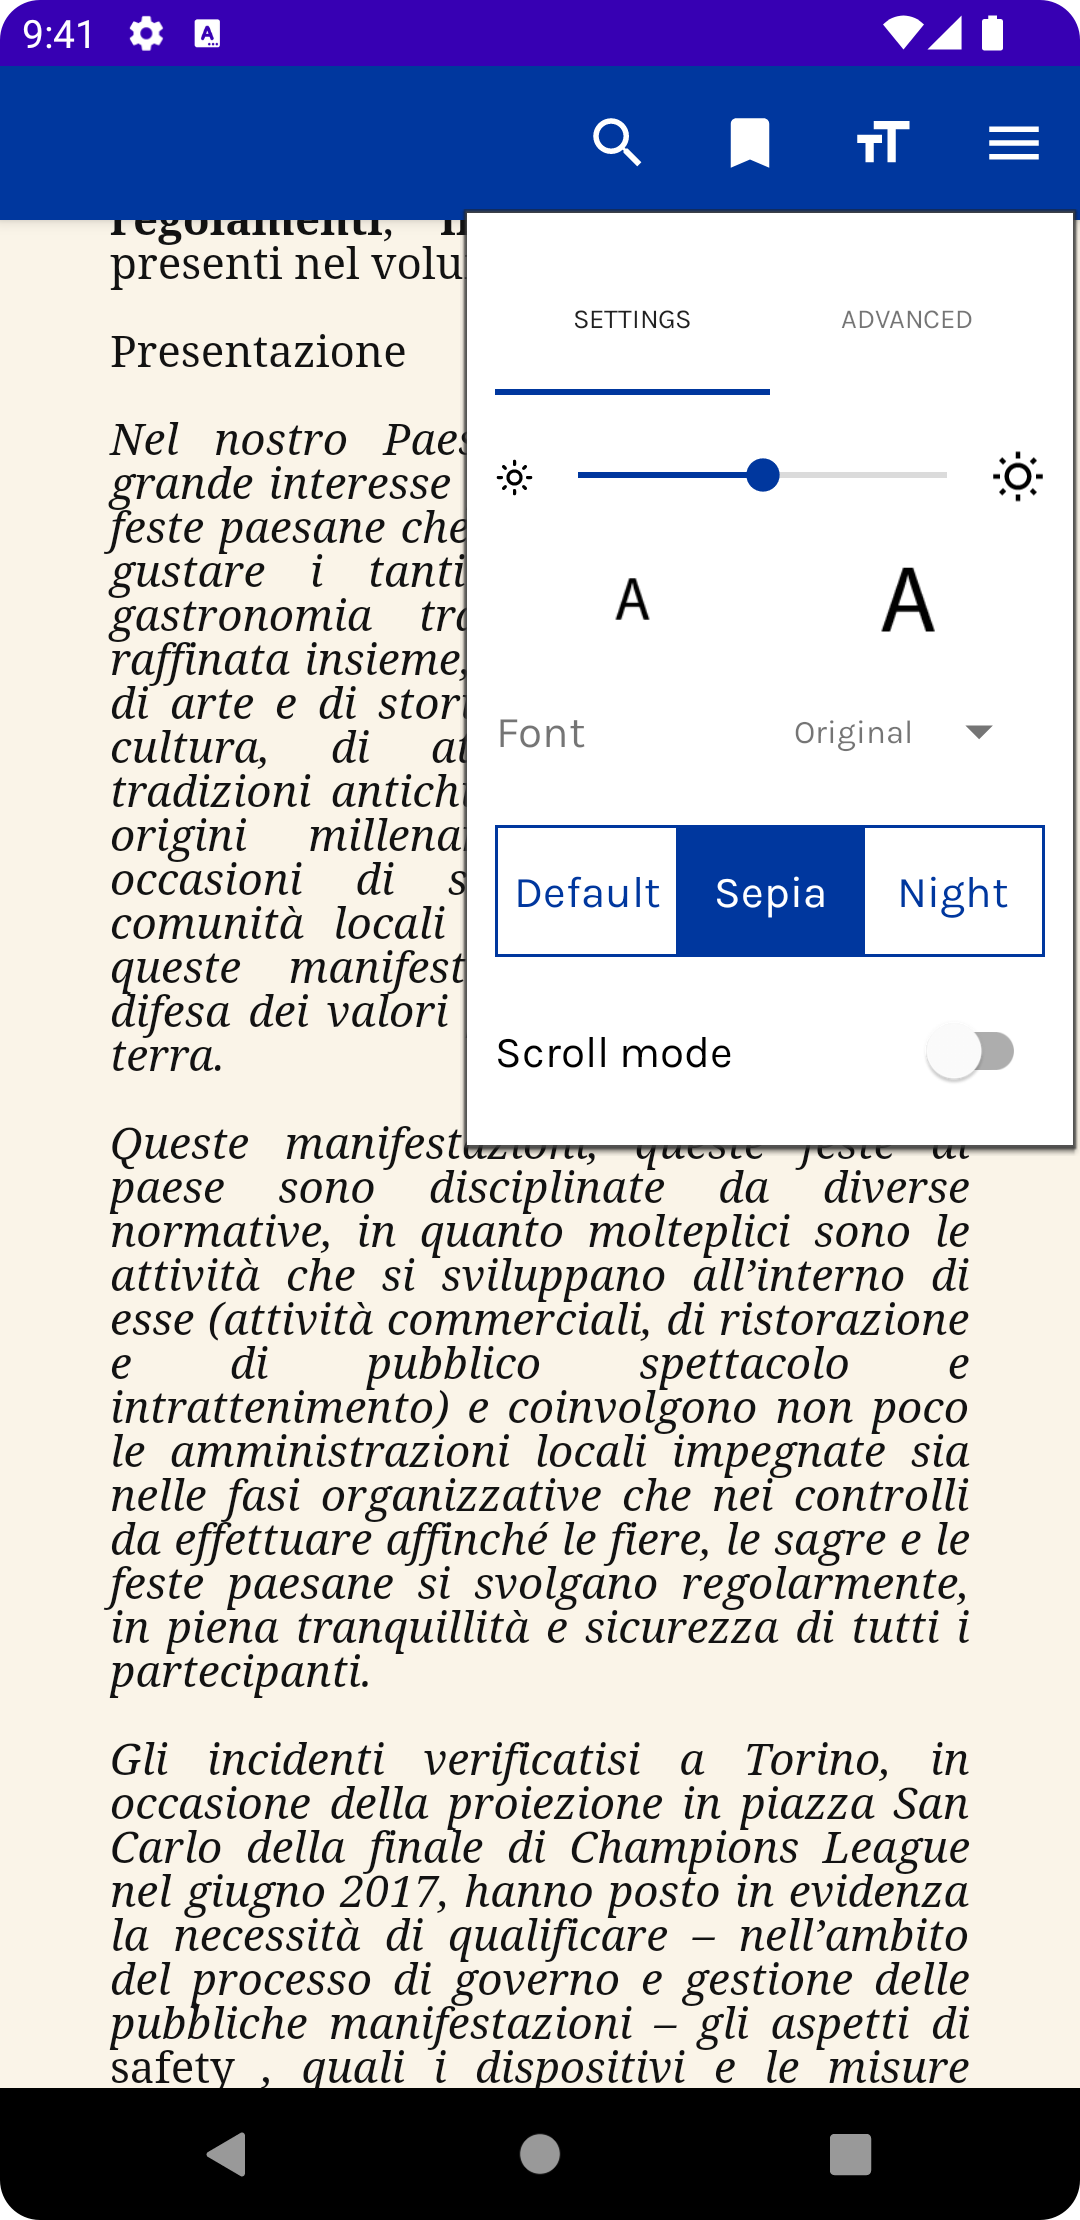
\includegraphics[width=0.29\textwidth]{img/reader_settings.png}
                \caption{Reader}
                \label{readersettings-android}
            \end{figure}
            
            \begin{figure}[H]
                \centering
                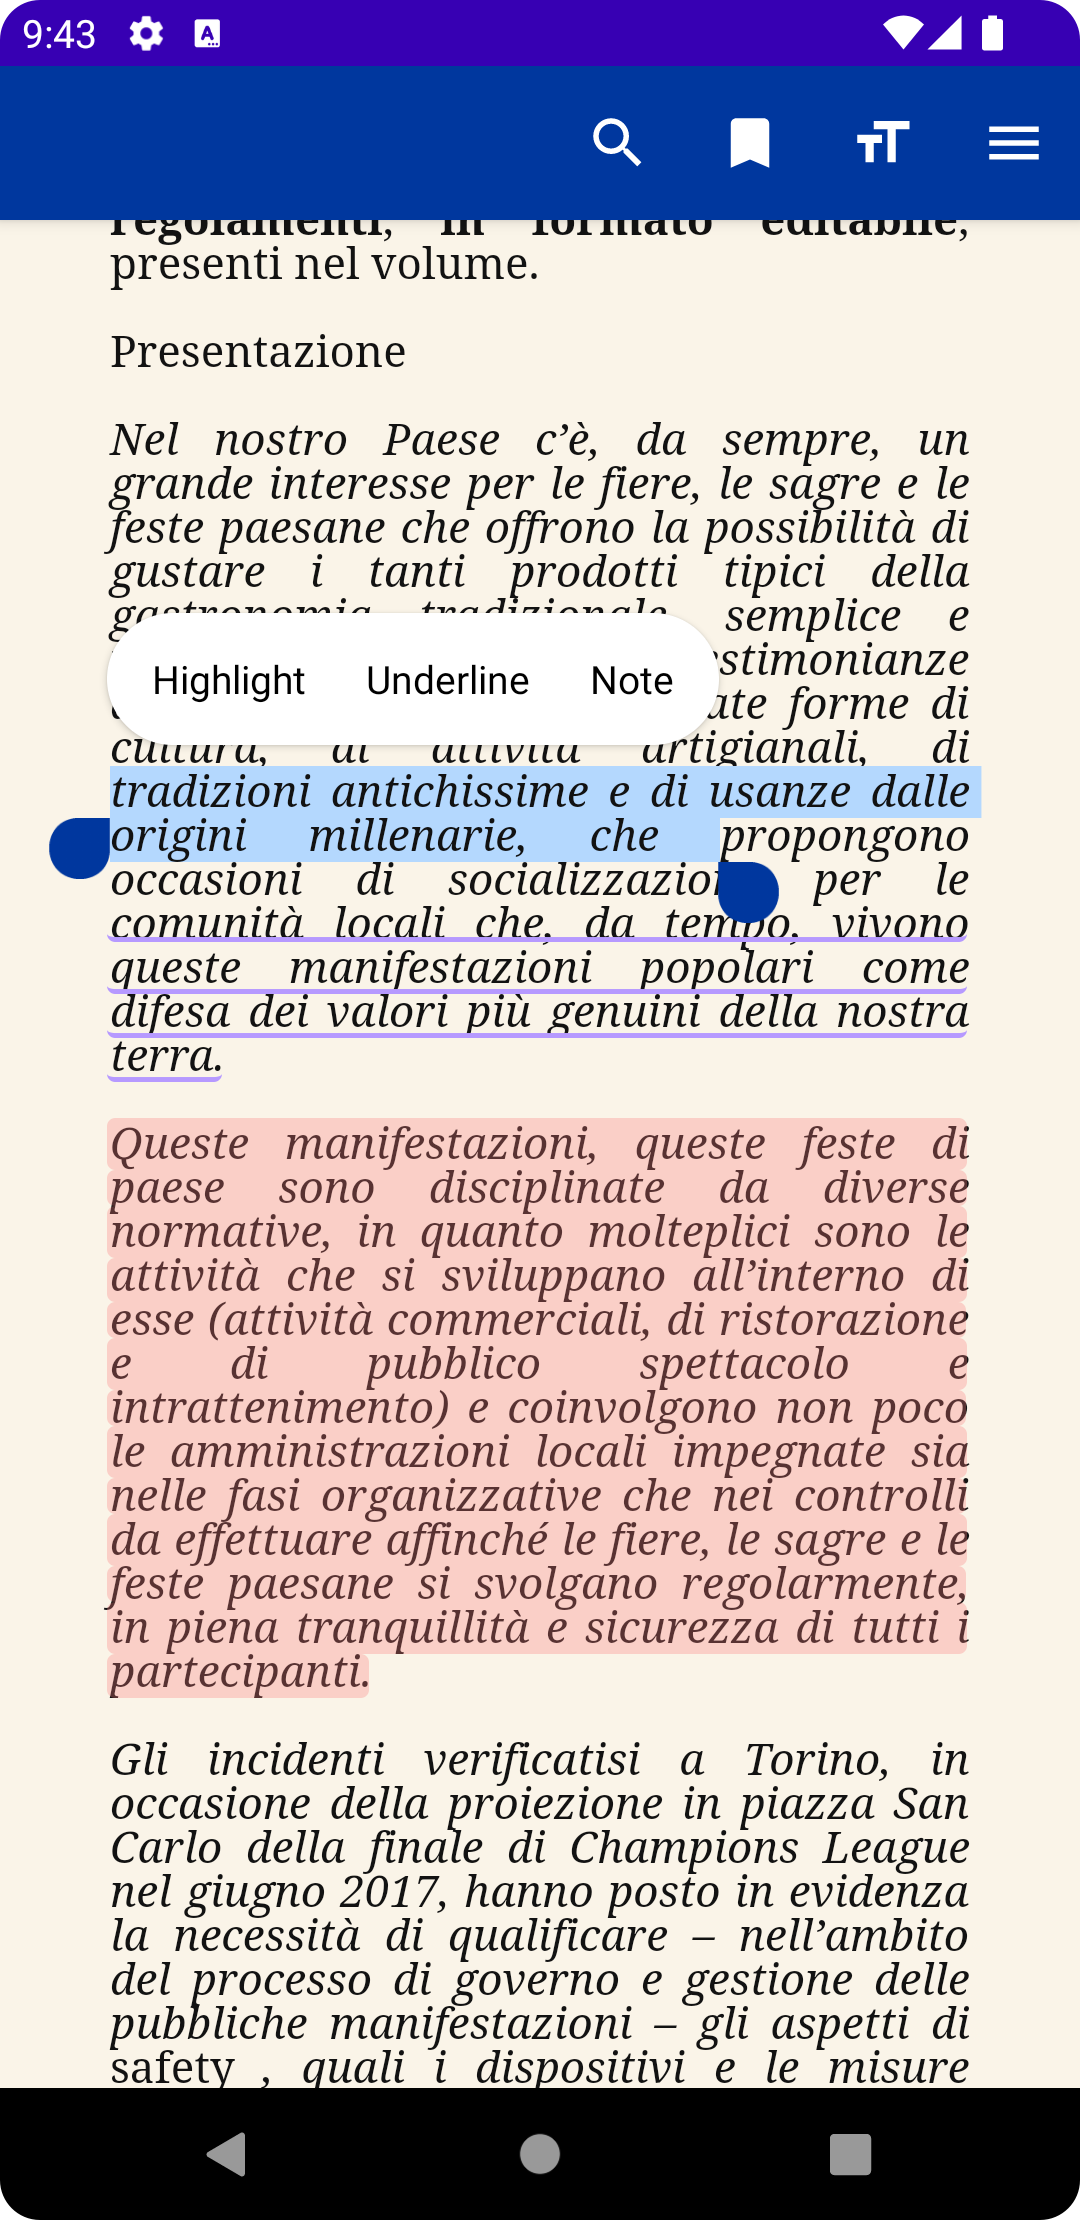
\includegraphics[width=0.29\textwidth]{img/annotations.png}
                \caption{Esempio di annotazioni, evidenziazioni, sottolineature, ...}
                \label{annotations-android}
            \end{figure}
            
            \begin{figure}[H]
                \centering
                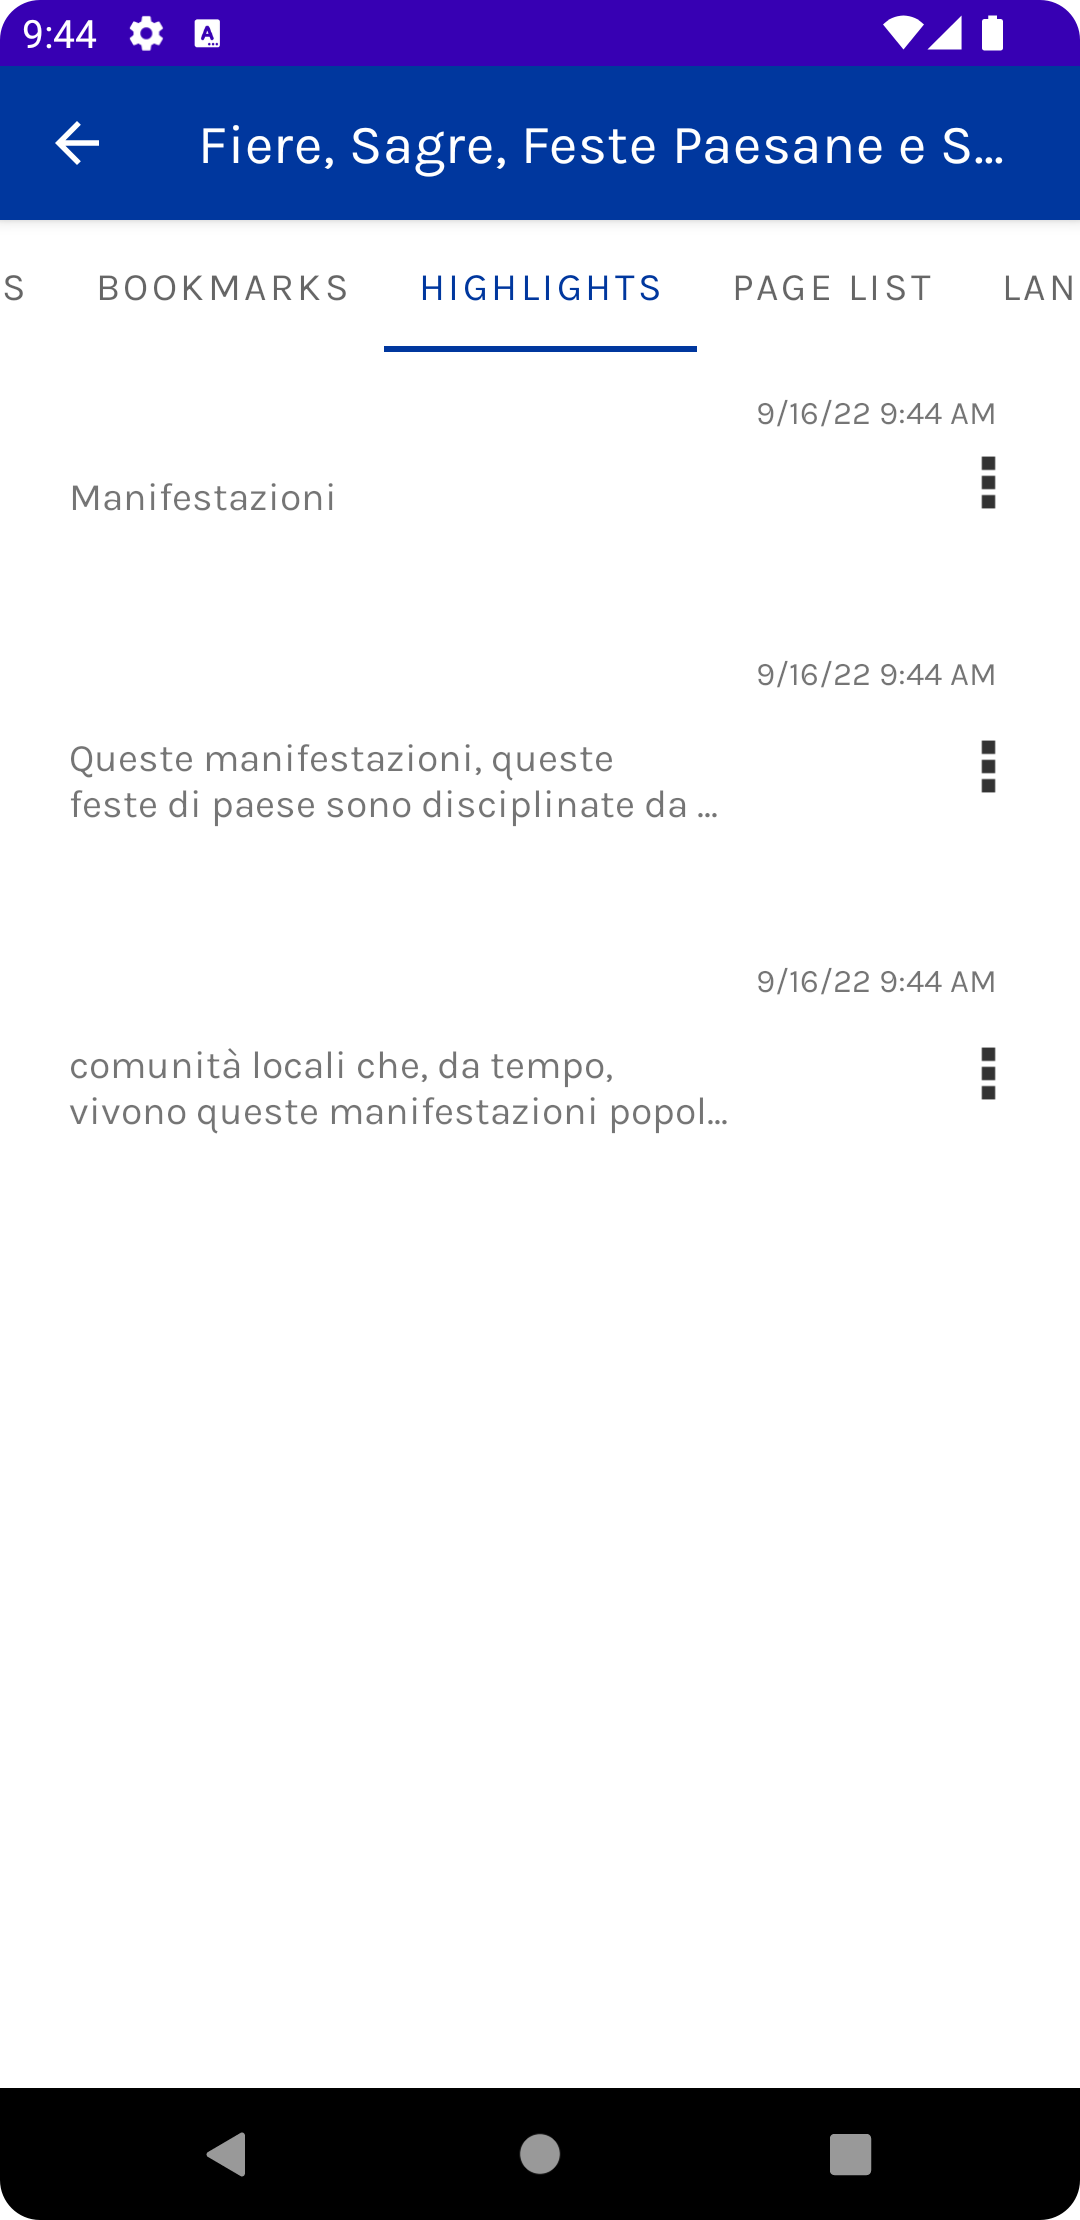
\includegraphics[width=0.29\textwidth]{img/annotation2.png}
                \caption{Annotazioni}
                \label{annotation2-android}
            \end{figure}

            \begin{figure}[H]
                \centering
                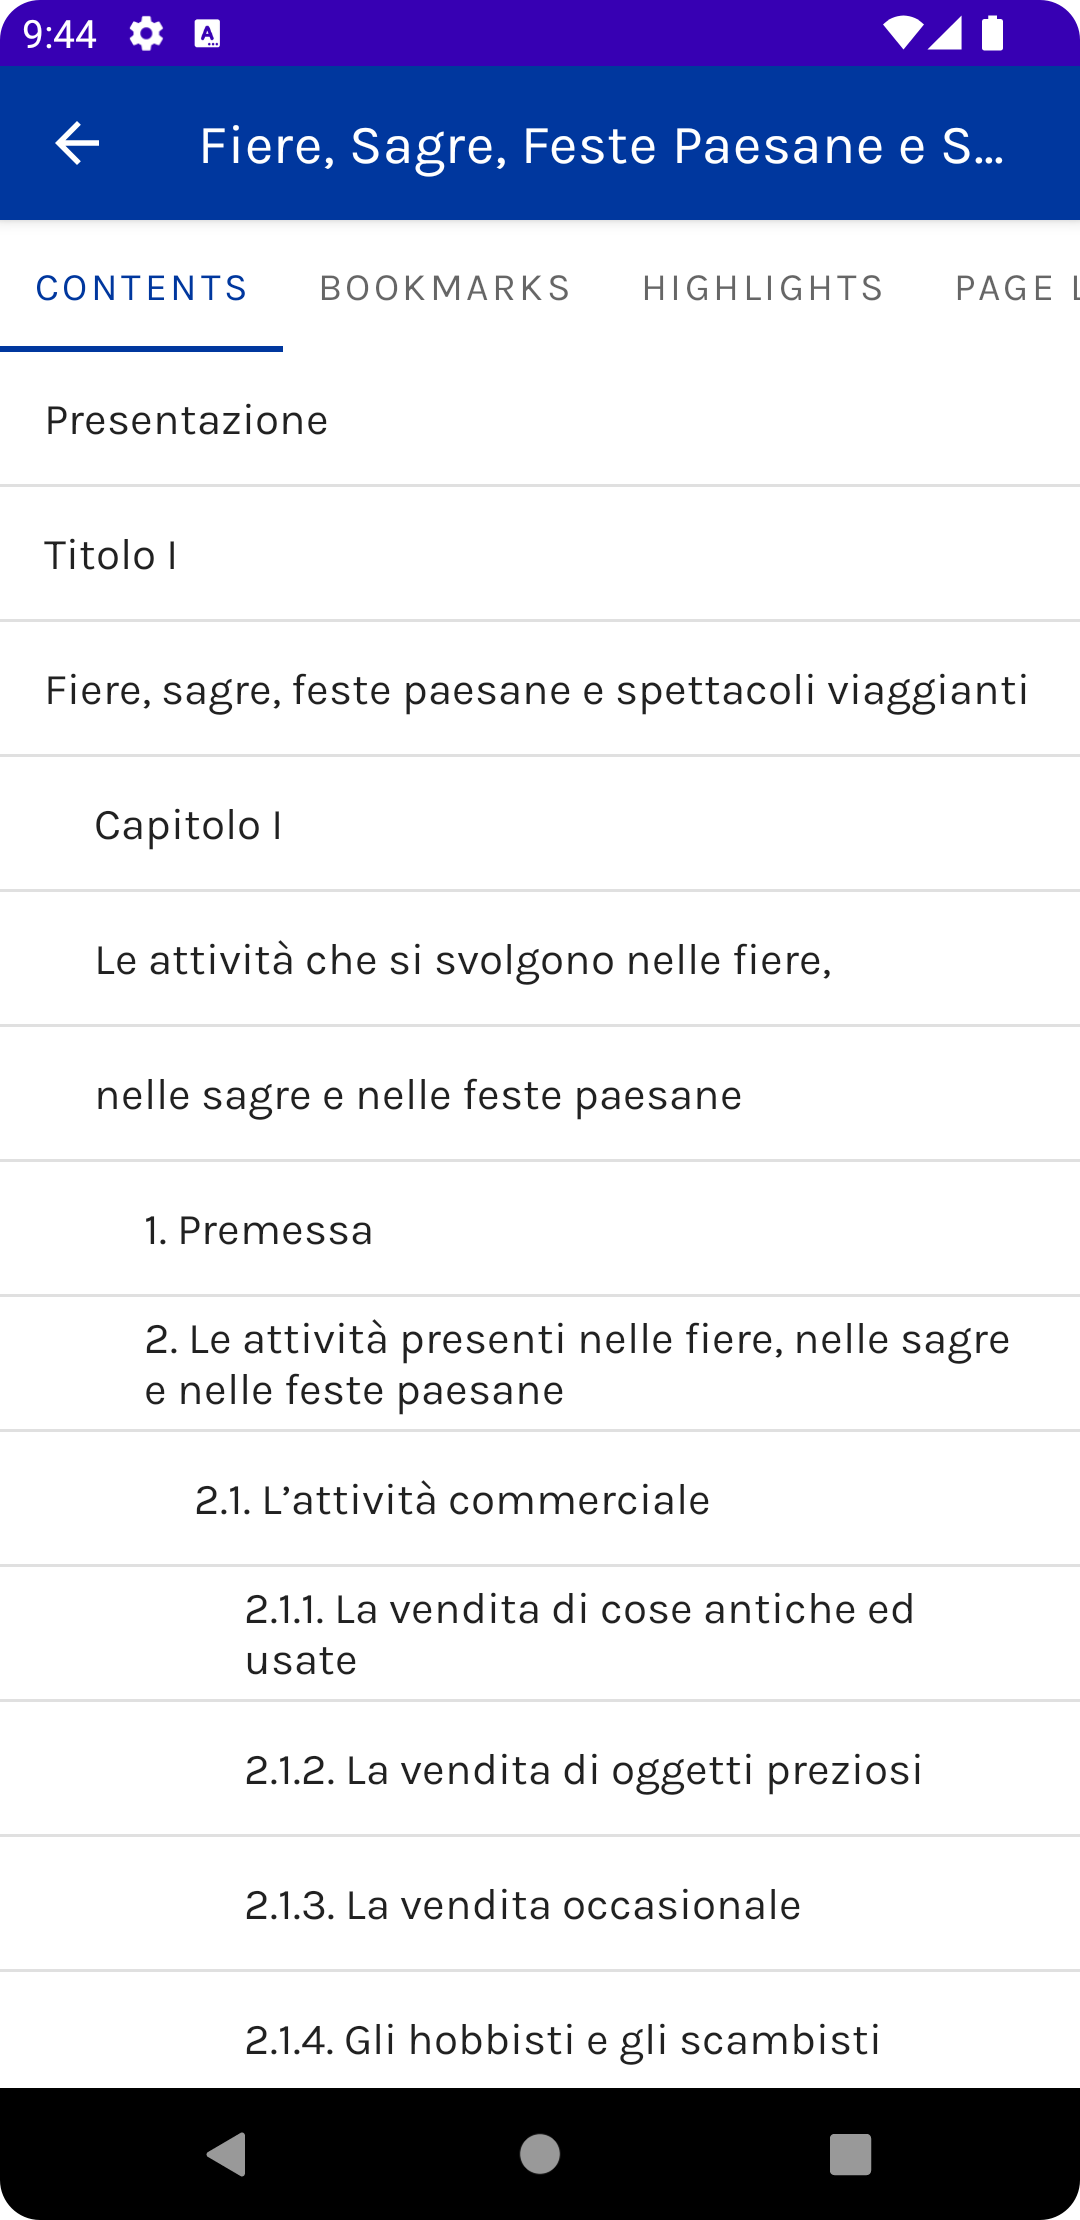
\includegraphics[width=0.29\textwidth]{img/toc.png}
                \caption{Elenco dei contenuti (TOC) del documento}
                \label{toc-android}
            \end{figure}
            
            \begin{figure}[H]
                \centering
                
\includegraphics[width=0.29\textwidth]{img/ricerca_testo.png}
                \caption{Ricerca testuale nel contenuto del documento}
                \label{ricerca_testo-android}
            \end{figure}
            
            \begin{figure}[H]
                \centering
                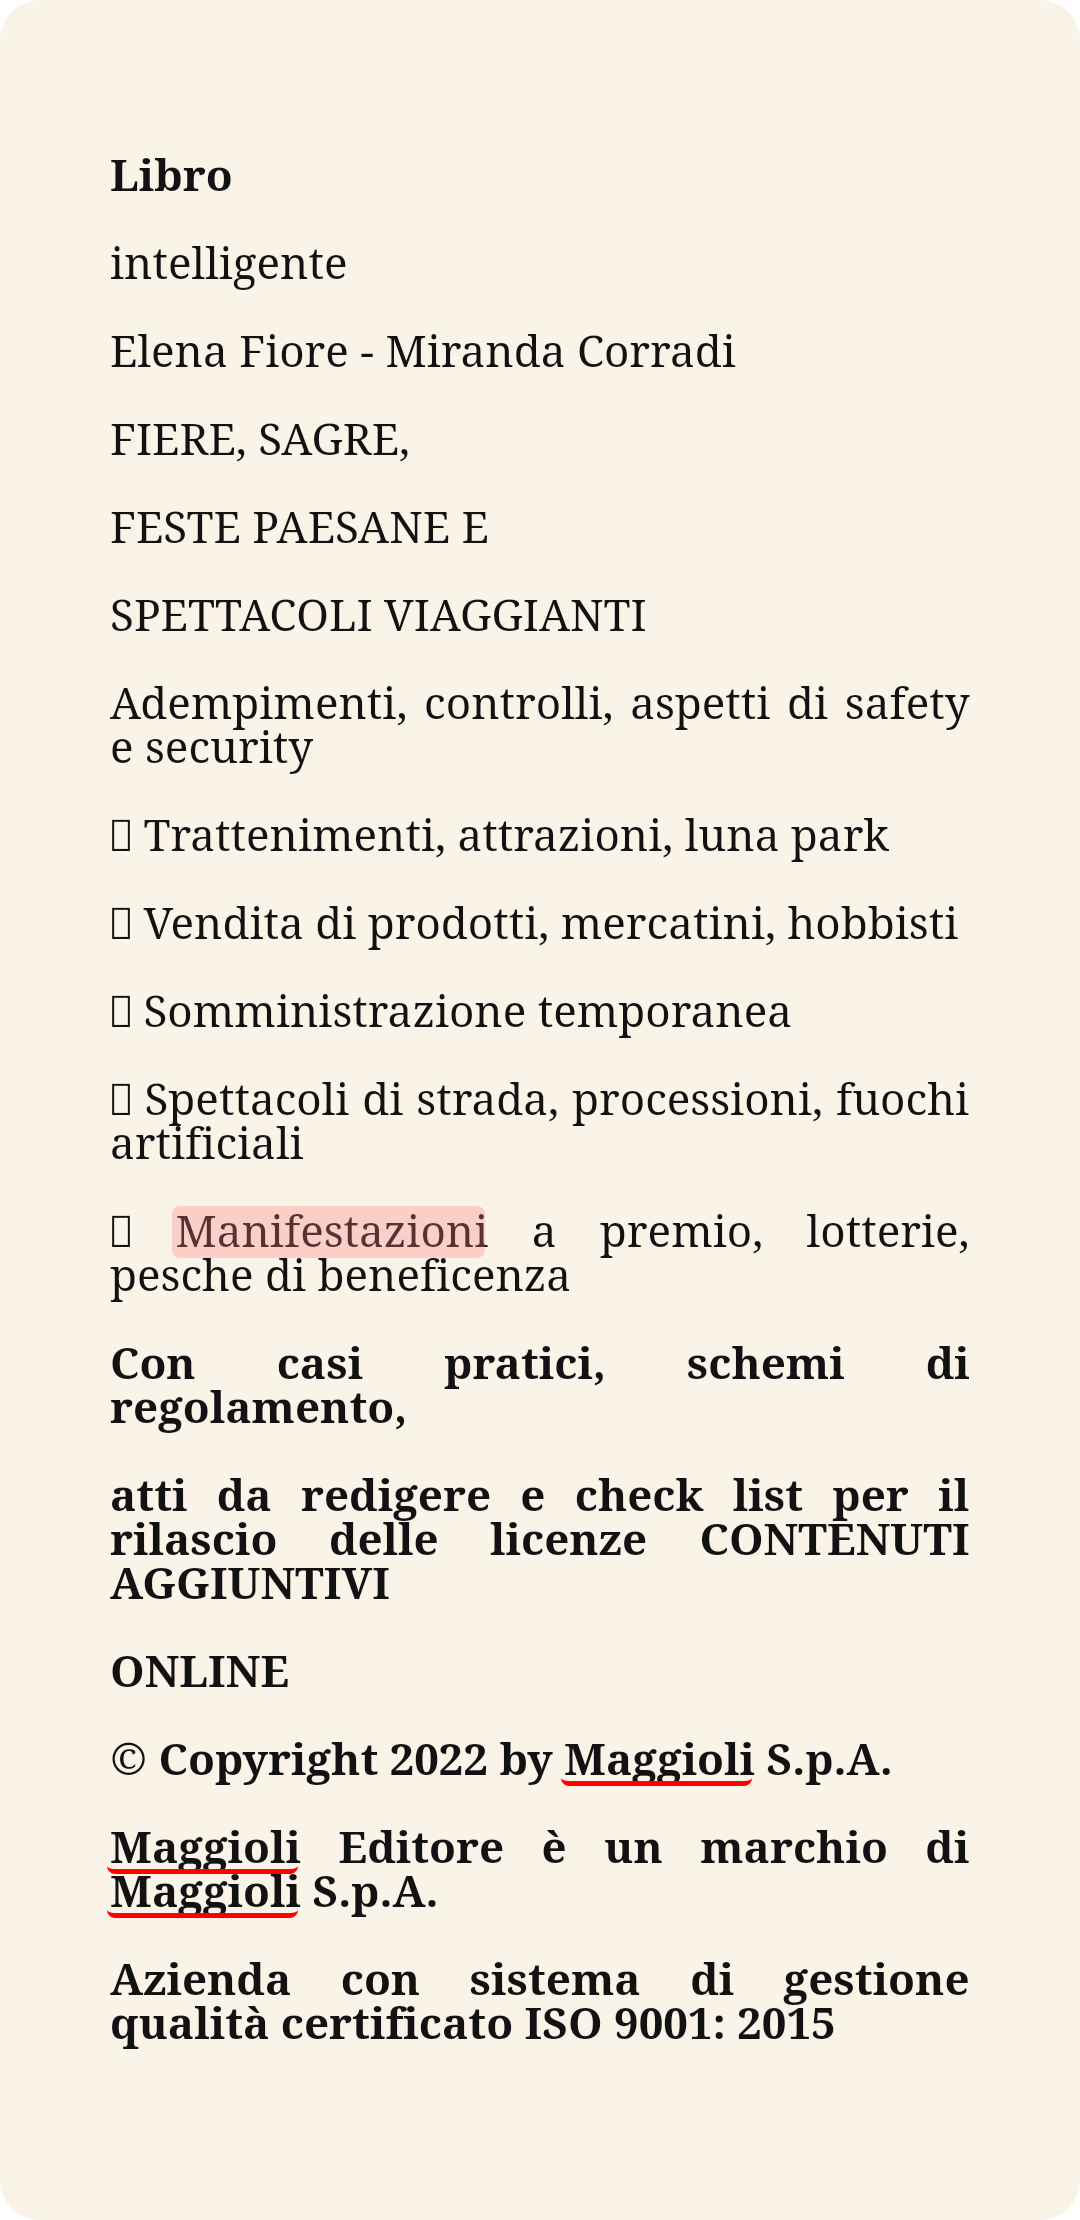
\includegraphics[width=0.29\textwidth]{img/ricerca_testo2.png}
                \caption{Evidenziazioni automatiche delle occorrenze del testo cercato}
                \label{ricerca_testo2-android}
            \end{figure}
\end{multicols}

\subsection{Applicazione iOS}
Terminato lo sviluppo dell'applicazione Android è possibile dedicarsi all'applicazione iOS,
per la quale rimangono valide le stesse considerazioni fatte sul processo e sull'architettura del caso di studio ma con la necessità di qualche intervento per il corretto funzionamento del framework KMM. 
Il progetto XCode\footnote{\href{https://github.com/paganellif/DevOps-per-applicazioni-mobile-un-caso-di-studio-industriale/tree/6-sviluppo-applicazione-maggioliebook/maggioliEbookApp/iosMaggioliEbookApp}{https://github.com/paganellif/DevOps-per-applicazioni-mobile-un-caso-di-studio-industriale/tree/6-sviluppo-applicazione-maggioliebook/maggioliEbookApp/iosMaggioliEbookApp}} di partenza per l'applicazione iOS è stato generato all'inizio della fase di sviluppo con l'inizializzazione dell'intero progetto tramite il plugin Gradle KMM per l'IDE Android Studio.

Per poter utilizzare il codice Kotlin del modulo condiviso nel codice Swift dell'applicazione iOS è necessario generare due tipi di pacchetto: 
(\textit{i}) framework di sviluppo per l'IDE XCode e (\textit{ii}) libreria CocoaPods da includere come dipendenza di progetto. 
Il framework di sviluppo può essere creato tramite l'apposito task \textit{embedAndSignPodAppleFrameworkForXCode} disponibile tramite il plugin Gradle KMM. 
Questo task permette di definire la modalità di compilazione, 
la versione e la posizione del framework.

\subsubsection*{CocoaPods}
Come anticipato nel capitolo \ref{ch:app-multiplatform}, 
CocoaPods è un dependency manager per progetti Swift e Objective-C scritto in Ruby. 
Le dipendenze, 
chiamate \textit{Pods}, 
sono definite nel file \textit{Podfile} nella root di progetto. 
Il pod shared viene generato durante la fase di impacchettamento del modulo shared tramite l’esecuzione del task Gradle \textit{assemble} per il quale sono definiti appositi sotto-task per svolgere questo compito.

Il seguente codice\footnote{\href{https://github.com/paganellif/DevOps-per-applicazioni-mobile-un-caso-di-studio-industriale/blob/6-sviluppo-applicazione-maggioliebook/maggioliEbookApp/iosMaggioliEbookApp/Podfile}{https://github.com/paganellif/DevOps-per-applicazioni-mobile-un-caso-di-studio-industriale/blob/6-sviluppo-applicazione-maggioliebook/maggioliEbookApp/iosMaggioliEbookApp/Podfile}}, 
ovvero il contenuto del Podfile del progetto, 
definisce le dipendenze incluse nell'applicazione iOS sviluppata:

\begin{listing}[H]
    \inputminted{ruby}{code/Podfile}
    \caption{Dipendenze CocoaPods dell'applicazione iOS sviluppata}
\end{listing}

A questo punto è possibile importare i moduli nel codice Swift e sviluppare l'applicazione utilizzando le funzionalità fornite dall'IDE XCode come per una qualsiasi libreria Swift importata. 
I task forniti dal plugin Gradle KMM a supporto dello sviluppo iOS tramite il dependency manager CocoaPods sono:

\begin{itemize}
    \item \textbf{podDownload} - Scarica le dipendenze CocoaPods senza effettuarne l'installazione.
    
    \item \textbf{podImport} - Task di utility utilizzato da altri task per l'import delle dipendenze.
    
    \item \textbf{podInstall} - Esegue l'installazione dei pod, in modo equivalente all'esecuzione del comando \textit{pod install}.
    
    \item \textbf{podPublishDebugXCFramework} - Crea il framework XCFramework in modalità debug (chiamato dal task \textit{embedAndSignPodAppleFrameworkForXcode}).
    
    \item \textbf{podPublishReleaseXCFramework} - Crea il framework XCFramework in modalità release (chiamato dal task \textit{embedAndSignPodAppleFrameworkForXcode}).
    
    \item \textbf{podPublishXCFramework} - Crea i framework XCFrameworc in entrambe le modalità.
    
    \item \textbf{podspec} - Genera il file \textit{podspec}\footnote{\href{https://guides.cocoapods.org/syntax/podspec.html}{https://guides.cocoapods.org/syntax/podspec.html}}, utile all'importazione del pod nell'applicazione iOS.
\end{itemize}

\subsubsection*{Navigator Architecture}
L'architettura dell'applicazione iOS sviluppata segue lo stesso pattern utilizzato nella versione Android ed è conosciuto col nome \textit{Navigator}. 
Tramite il costrutto \textit{NavigationView}\footnote{\href{https://developer.apple.com/documentation/swiftui/navigationview}{https://developer.apple.com/documentation/swiftui/navigationview}} è possibile definire una schermata ``contenitore'' per le viste dei percorsi di navigazione all'interno dell'applicazione.

Le schermate da realizzare sono le stesse individuate nella progettazione della UX/UI ed è necessario utilizzare i \textit{NavigationLink}\footnote{\href{https://developer.apple.com/documentation/swiftui/navigationlink}{https://developer.apple.com/documentation/swiftui/navigationlink}} per poterle navigare nell'architettura scelta.
I NavigationLink, i quali identificano una specifica transizione di schermata da quella attuale a quella di destinazione, sono definiti nel componente \textit{NavController}\footnote{\href{https://github.com/paganellif/DevOps-per-applicazioni-mobile-un-caso-di-studio-industriale/blob/6-sviluppo-applicazione-maggioliebook/maggioliEbookApp/iosMaggioliEbookApp/iosMaggioliEbookApp/Common/NavController.swift}{https://github.com/paganellif/DevOps-per-applicazioni-mobile-un-caso-di-studio-industriale/blob/6-sviluppo-applicazione-maggioliebook/maggioliEbookApp/iosMaggioliEbookApp/\\iosMaggioliEbookApp/Common/NavController.swift}} ma vengono attivati dal componente \textit{Sidebar}\footnote{\href{https://github.com/paganellif/DevOps-per-applicazioni-mobile-un-caso-di-studio-industriale/blob/6-sviluppo-applicazione-maggioliebook/maggioliEbookApp/iosMaggioliEbookApp/iosMaggioliEbookApp/Common/Sidebar.swift}{https://github.com/paganellif/DevOps-per-applicazioni-mobile-un-caso-di-studio-industriale/blob/6-sviluppo-applicazione-maggioliebook/maggioliEbookApp/iosMaggioliEbookApp/\\iosMaggioliEbookApp/Common/Sidebar.swift}}. 
A differenza di Jetpack Compose, i
l toolkit utilizzato nello sviluppo della UI Android, 
SwiftUI non fornisce nativamente dei costrutti per la realizzazione di schermate con scroll infinito e dati paginati (come descritto nella sezione \ref{pagingsec}): 
per questo motivo è stata necessaria l'implementazione di un meccanismo ad-hoc\footnote{\href{https://github.com/paganellif/DevOps-per-applicazioni-mobile-un-caso-di-studio-industriale/blob/6-sviluppo-applicazione-maggioliebook/maggioliEbookApp/iosMaggioliEbookApp/iosMaggioliEbookApp/Home/HomeViewModel.swift}{https://github.com/paganellif/DevOps-per-applicazioni-mobile-un-caso-di-studio-industriale/blob/6-sviluppo-applicazione-maggioliebook/maggioliEbookApp/iosMaggioliEbookApp/\\iosMaggioliEbookApp/Home/HomeViewModel.swift}} per la gestione di questo scenario.

\begin{figure}[H]
\centering
    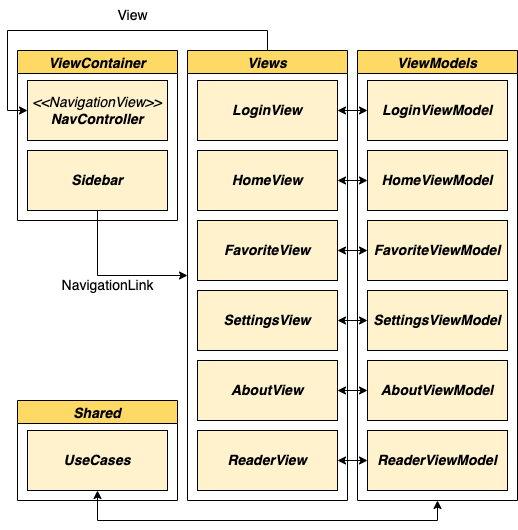
\includegraphics[width=0.63\textwidth]{img/navigator-arch-ios.png}
    \caption{Architettura Navigator adottata per l'applicazione iOS}
    \label{iosarchapp}
\end{figure}

\subsubsection*{Integrazione iOS-Shared}
\label{integrazione-ios-shared}
Grazie al framework Kotlin Multiplatform Mobile e ai realtivi plugin Gradle di supporto è stato possibile completare con successo una serie di compilazioni (fig. \ref{kotlin-native-compile}) in grado di ``trasformare'' codice Kotlin in codice Swift. 
Nonostante il codice Kotlin venga compilato correttamente in codice Swift, 
per ottenere codice funzionante in grado di svolgere le stesse funzionalità sviluppate nell'applicazione Android è stato necessario svolgere dell'ulteriore lavoro d'integrazione, 
riguardante principalmente la computazione asincrona e i tipi di dato:

\begin{itemize}
    \item Realizzazione di un metodo specifico, chiamato \textit{invokeNative}\footnote{\href{https://github.com/paganellif/DevOps-per-applicazioni-mobile-un-caso-di-studio-industriale/blob/6-sviluppo-applicazione-maggioliebook/maggioliEbookApp/shared/src/commonMain/kotlin/it/filo/maggioliebook/usecase/core/ConvertPdf2EpubUseCase.kt}{https://github.com/paganellif/DevOps-per-applicazioni-mobile-un-caso-di-studio-industriale/blob/6-sviluppo-applicazione-maggioliebook/maggioliEbookApp/shared/src/commonMain/\\kotlin/it/filo/maggioliebook/usecase/core/ConvertPdf2EpubUseCase.kt}}, nel modulo condiviso per l'invocazione dei casi d'uso. Le \textit{coroutines} di Kotlin vengono infatti mappate da KMM in funzioni con callbacks, chiamate \textit{completion handlers} e non esiste modo di definire un \textit{CoroutineScope} in Swift. In questo modo è stato invece possibile definire uno scope per l'esecuzione del codice asincrono anche su target iOS.
    
    \item Impostazione del nuovo modello sperimentale di gestione della memoria nel file \textit{gradle.properties}\footnote{\href{https://github.com/paganellif/DevOps-per-applicazioni-mobile-un-caso-di-studio-industriale/blob/6-sviluppo-applicazione-maggioliebook/maggioliEbookApp/gradle.properties}{https://github.com/paganellif/DevOps-per-applicazioni-mobile-un-caso-di-studio-industriale/blob/6-sviluppo-applicazione-maggioliebook/maggioliEbookApp/gradle.properties}} per il modulo condiviso tramite la configurazione del parametro \textit{kotlin.native.binary.memoryModel=experimental}\footnote{\href{https://kotlinlang.org/docs/native-memory-manager.html}{https://kotlinlang.org/docs/native-memory-manager.html}}.
    
    \item Realizzazione di un metodo\footnote{\href{https://github.com/paganellif/DevOps-per-applicazioni-mobile-un-caso-di-studio-industriale/blob/6-sviluppo-applicazione-maggioliebook/maggioliEbookApp/shared/src/iosMain/kotlin/it/filo/maggioliebook/util/extensions/ByteArrayConverter.kt}{https://github.com/paganellif/DevOps-per-applicazioni-mobile-un-caso-di-studio-industriale/blob/6-sviluppo-applicazione-maggioliebook/maggioliEbookApp/shared/src/iosMain/kotlin/\\it/filo/maggioliebook/util/extensions/ByteArrayConverter.kt}} di conversione da \textit{ByteArray} Kotlin a \textit{NSData} Swift in modo da permettere la corretta gestione di dati binari, come ad esempio le immagini delle copertine e il contenuto EPUB delle pubblicazioni digitali nello specifico del caso di studio.
    
    \item Realizzazione di un metodo\footnote{\href{https://github.com/paganellif/DevOps-per-applicazioni-mobile-un-caso-di-studio-industriale/blob/6-sviluppo-applicazione-maggioliebook/maggioliEbookApp/iosMaggioliEbookApp/iosMaggioliEbookApp/Common/Extensions/Date.swift}{https://github.com/paganellif/DevOps-per-applicazioni-mobile-un-caso-di-studio-industriale/blob/6-sviluppo-applicazione-maggioliebook/maggioliEbookApp/iosMaggioliEbookApp/\\iosMaggioliEbookApp/Common/Extensions/Date.swift}} di gestione delle date e del tempo equivalente a quello utilizzato nel dominio modellato, in particolare per i tipi di dato utilizzati durante la persistenza dei dati tramite SqlDelight.
    
    \item Estensione\footnote{\href{https://github.com/paganellif/DevOps-per-applicazioni-mobile-un-caso-di-studio-industriale/blob/6-sviluppo-applicazione-maggioliebook/maggioliEbookApp/iosMaggioliEbookApp/iosMaggioliEbookApp/Common/Extensions/Libro.swift}{https://github.com/paganellif/DevOps-per-applicazioni-mobile-un-caso-di-studio-industriale/blob/6-sviluppo-applicazione-maggioliebook/maggioliEbookApp/iosMaggioliEbookApp/\\iosMaggioliEbookApp/Common/Extensions/Libro.swift}} delle entità di dominio per indicare l'identificativo utilizzato da Swift per ciclare su liste di elementi di quel tipo.
\end{itemize}

Grazie al lavoro aggiuntivo svolto è stato possibile utilizzare efficacemente il modulo condiviso all'interno dell'applicazione iOS, 
come ad esempio nel seguente caso\footnote{\href{https://github.com/paganellif/DevOps-per-applicazioni-mobile-un-caso-di-studio-industriale/blob/6-sviluppo-applicazione-maggioliebook/maggioliEbookApp/iosMaggioliEbookApp/iosMaggioliEbookApp/Common/CoverLoader.swift}{https://github.com/paganellif/DevOps-per-applicazioni-mobile-un-caso-di-studio-industriale/blob/6-sviluppo-applicazione-maggioliebook/maggioliEbookApp/iosMaggioliEbookApp/\\iosMaggioliEbookApp/Common/CoverLoader.swift}} asincrono di ottenimento e conversione della copertina di una pubblicazione digitale:

\begin{listing}[H]
    \inputminted{swift}{code/CoverLoader.swift}
    \caption{Esempio di utilizzo dei casi d'uso del modulo condiviso (computazione asincrona e gestione di dati binari)}
\end{listing}

\subsubsection*{Screenshot}
\begin{multicols}{3}
    \begin{figure}[H]
        \centering
        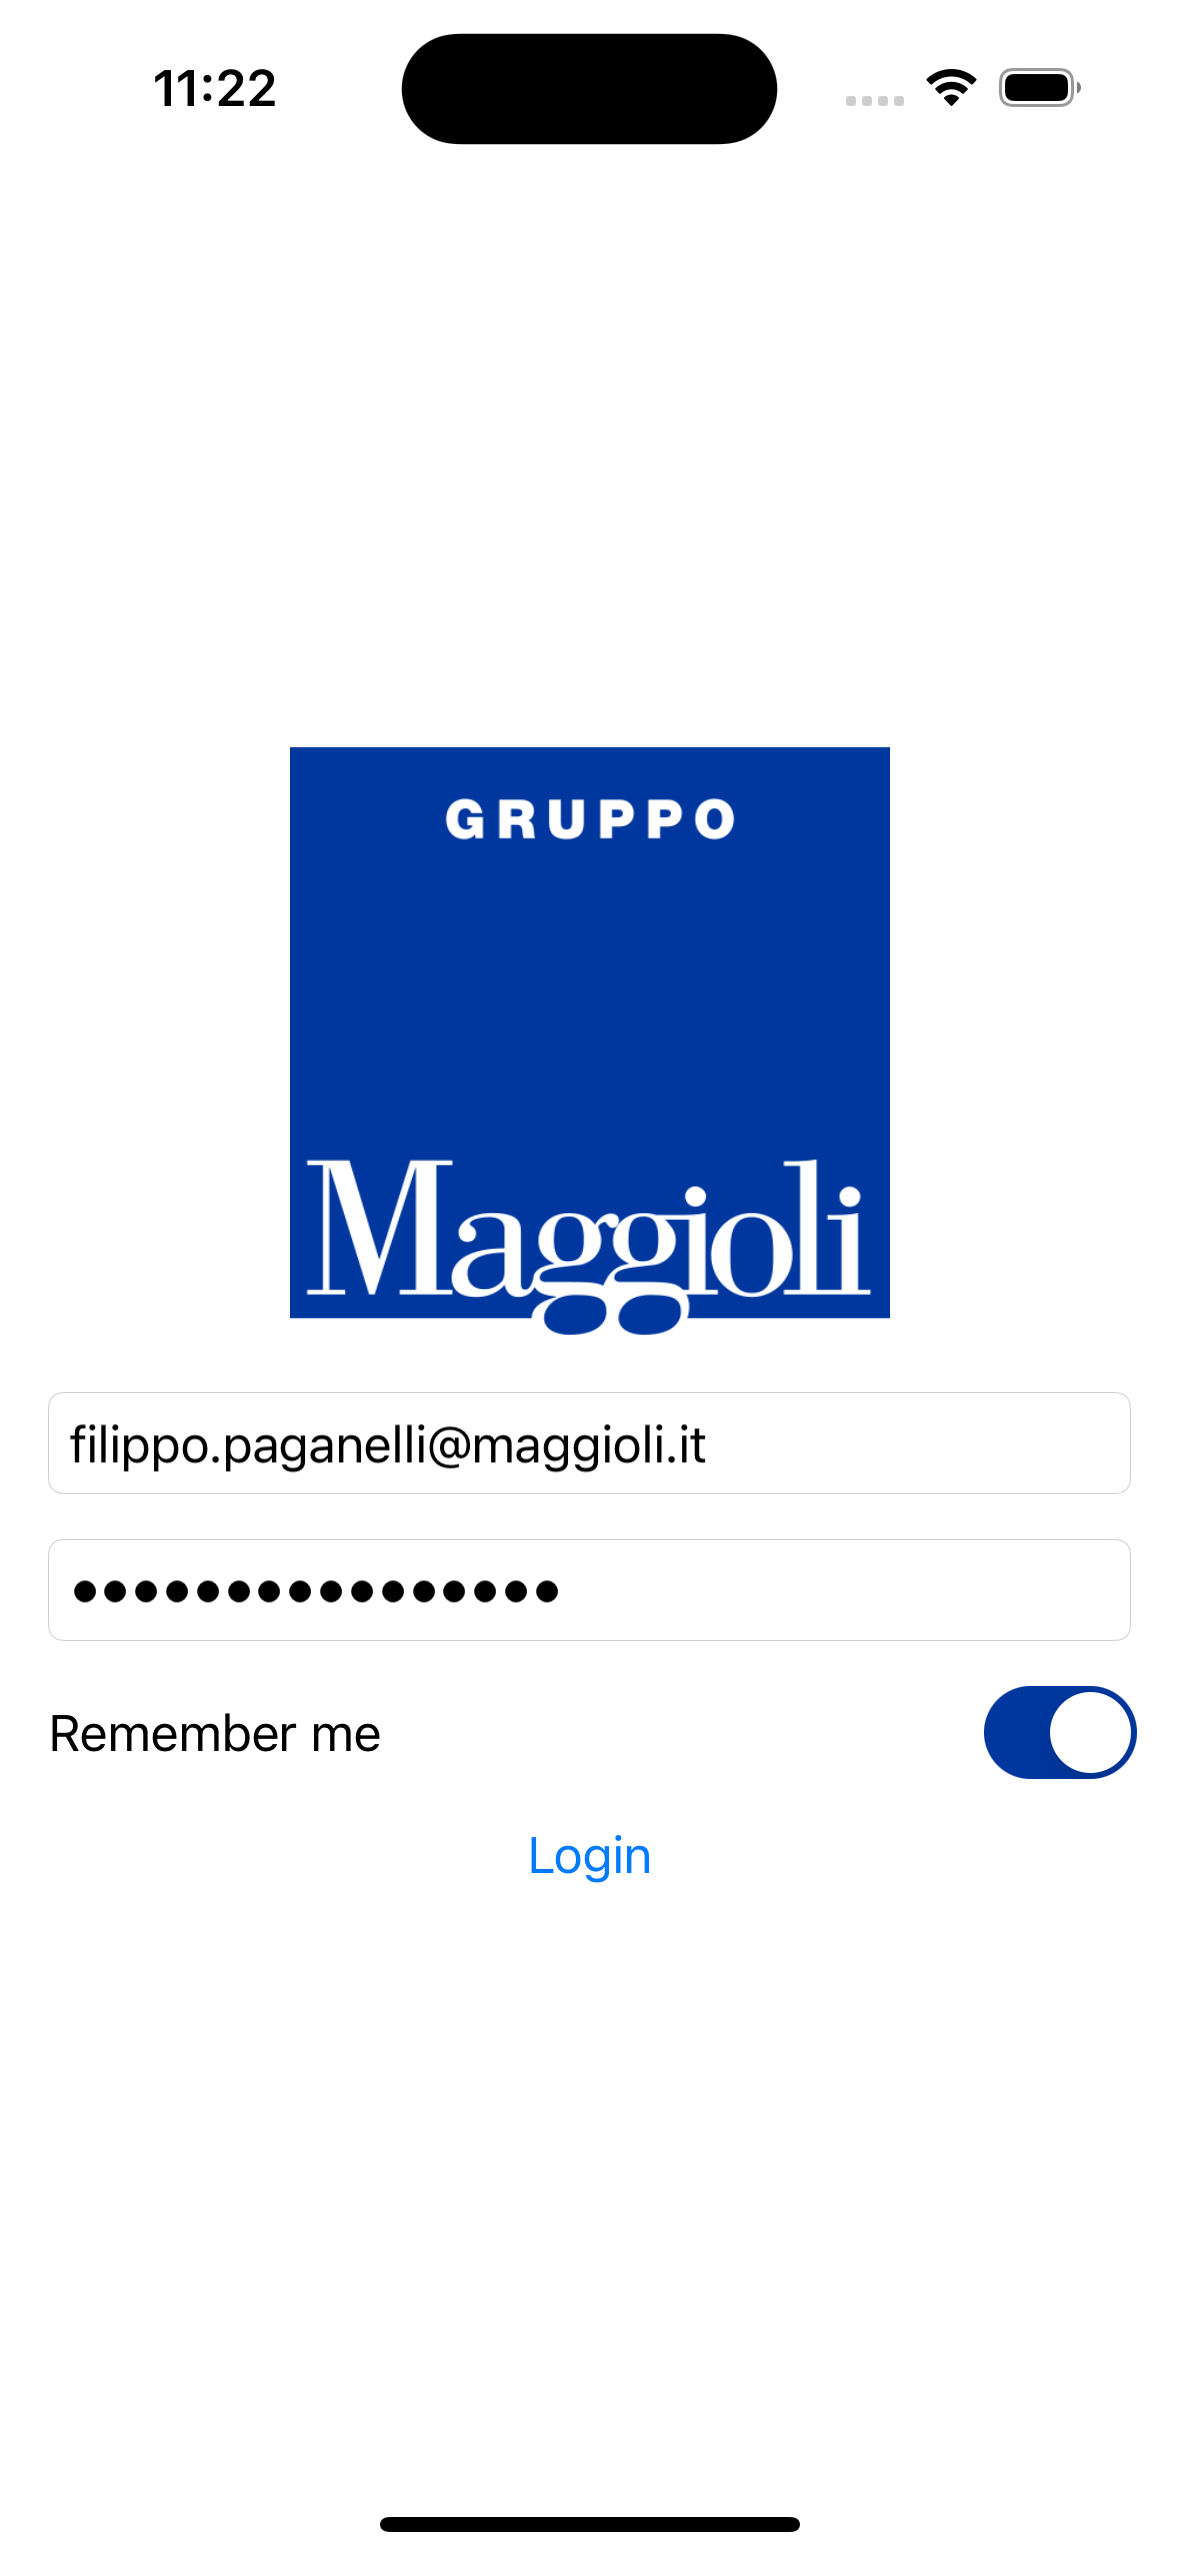
\includegraphics[width=0.26\textwidth]{img/Simulator Screen Shot - iPhone 14 Pro - 2022-10-05 at 11.22.08.png}
        \caption{Login}
        \label{login-ios}
    \end{figure}

    \begin{figure}[H]
        \centering
        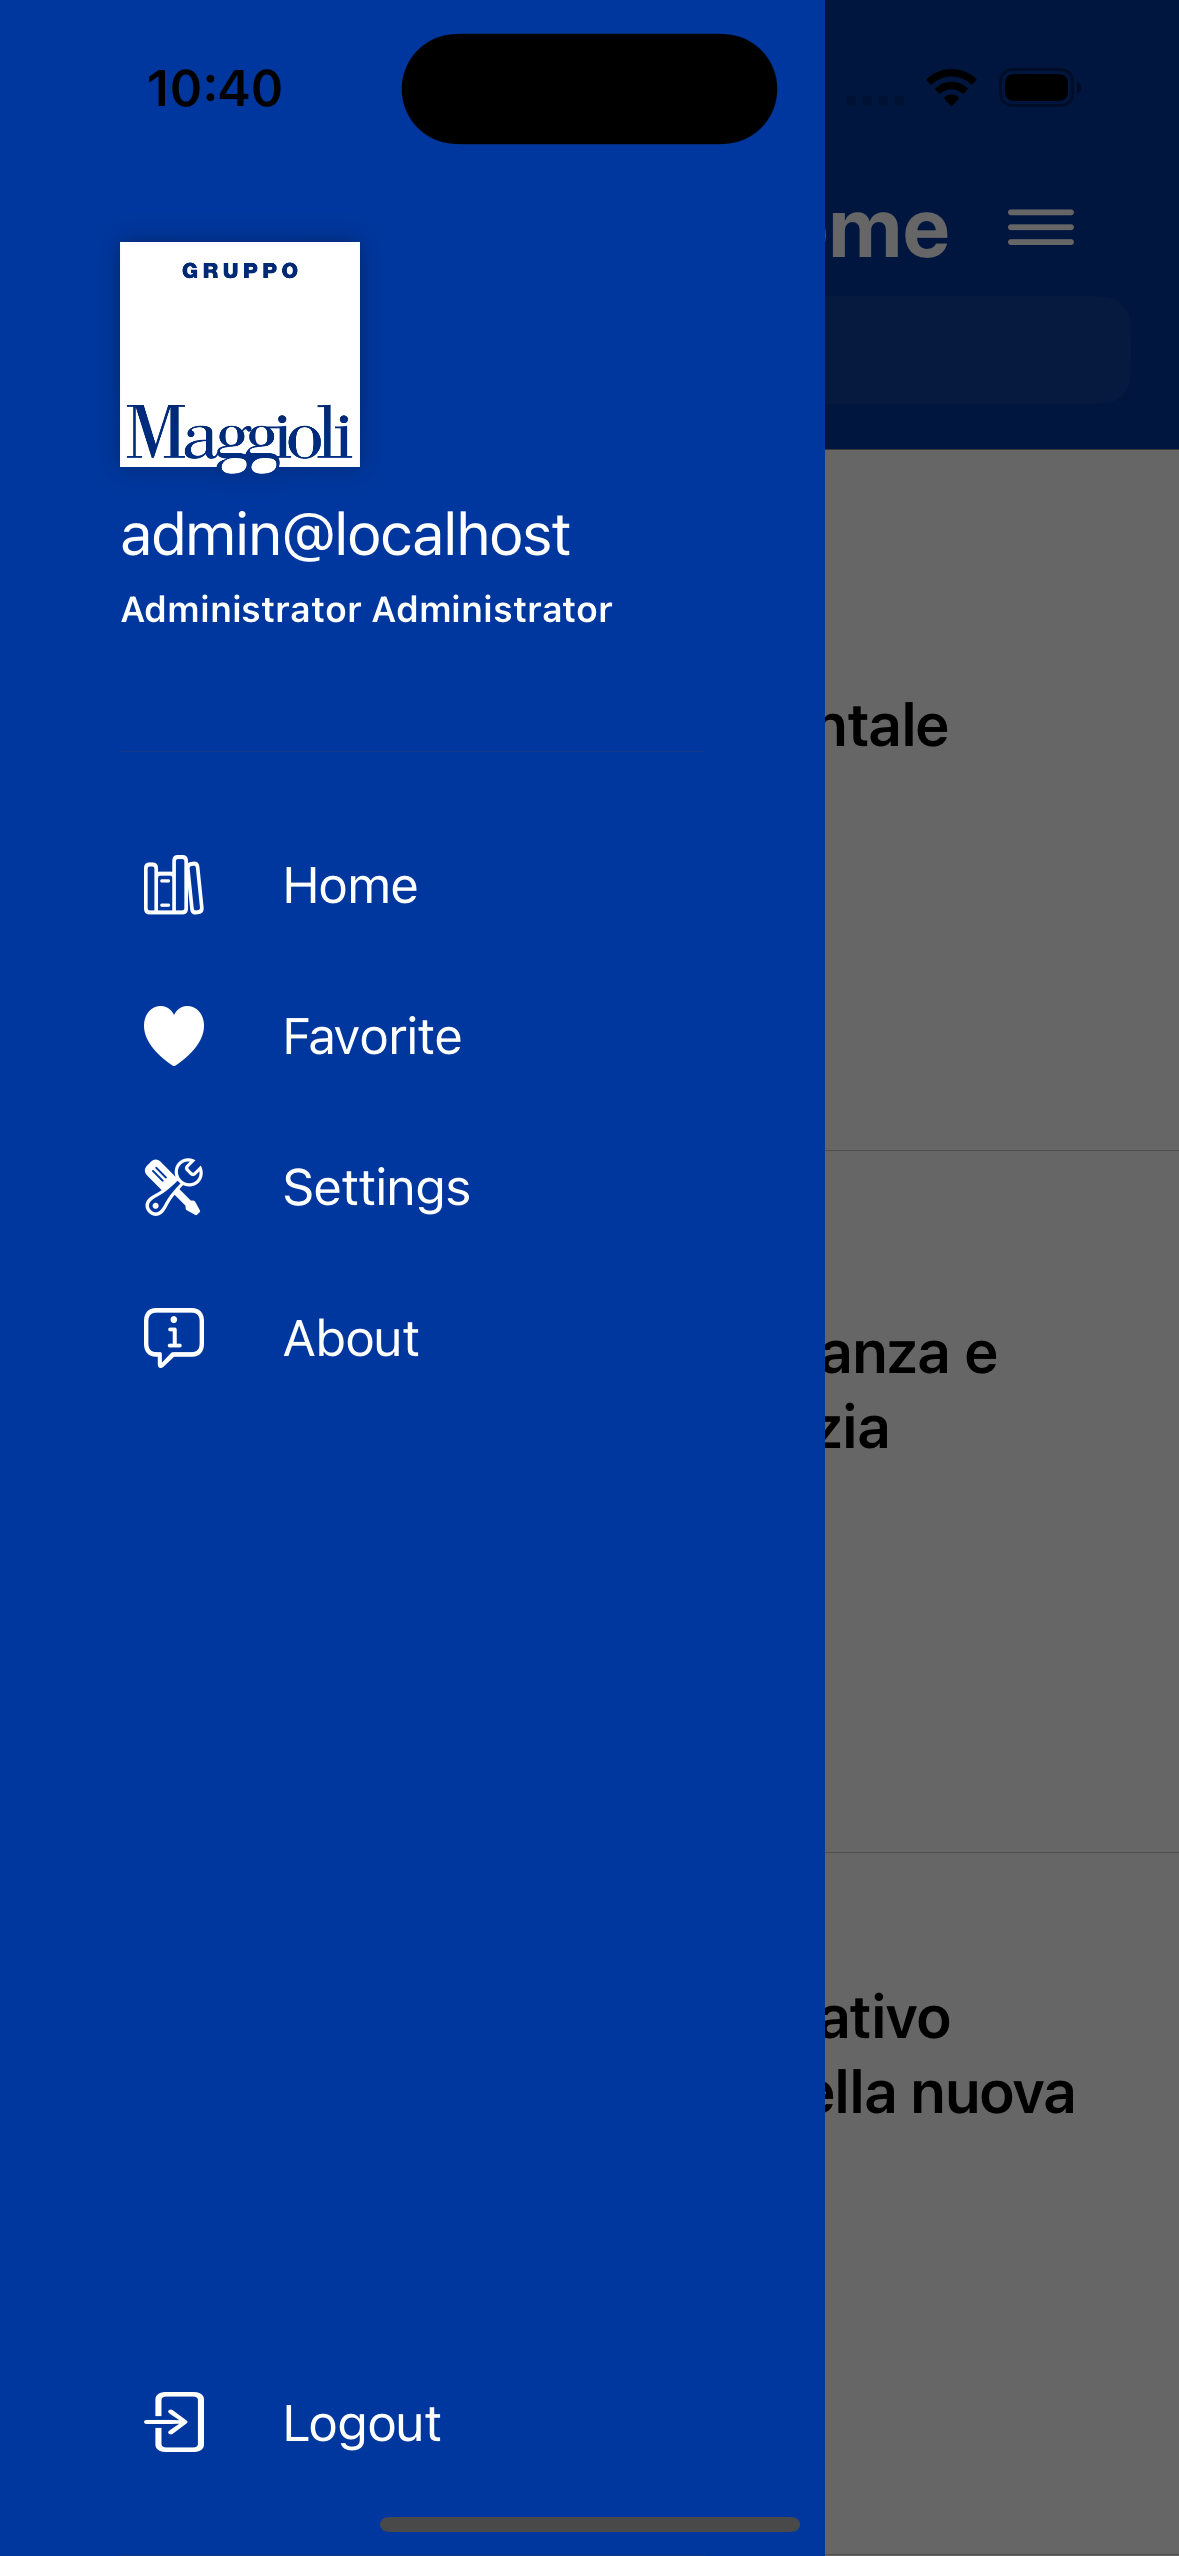
\includegraphics[width=0.26\textwidth]{img/Simulator Screen Shot - iPhone 14 Pro - 2022-10-05 at 10.40.04.png}
        \caption{Menu laterale - Sidenav}
        \label{sidenav-ios}
    \end{figure}
    
    \begin{figure}[H]
        \centering
        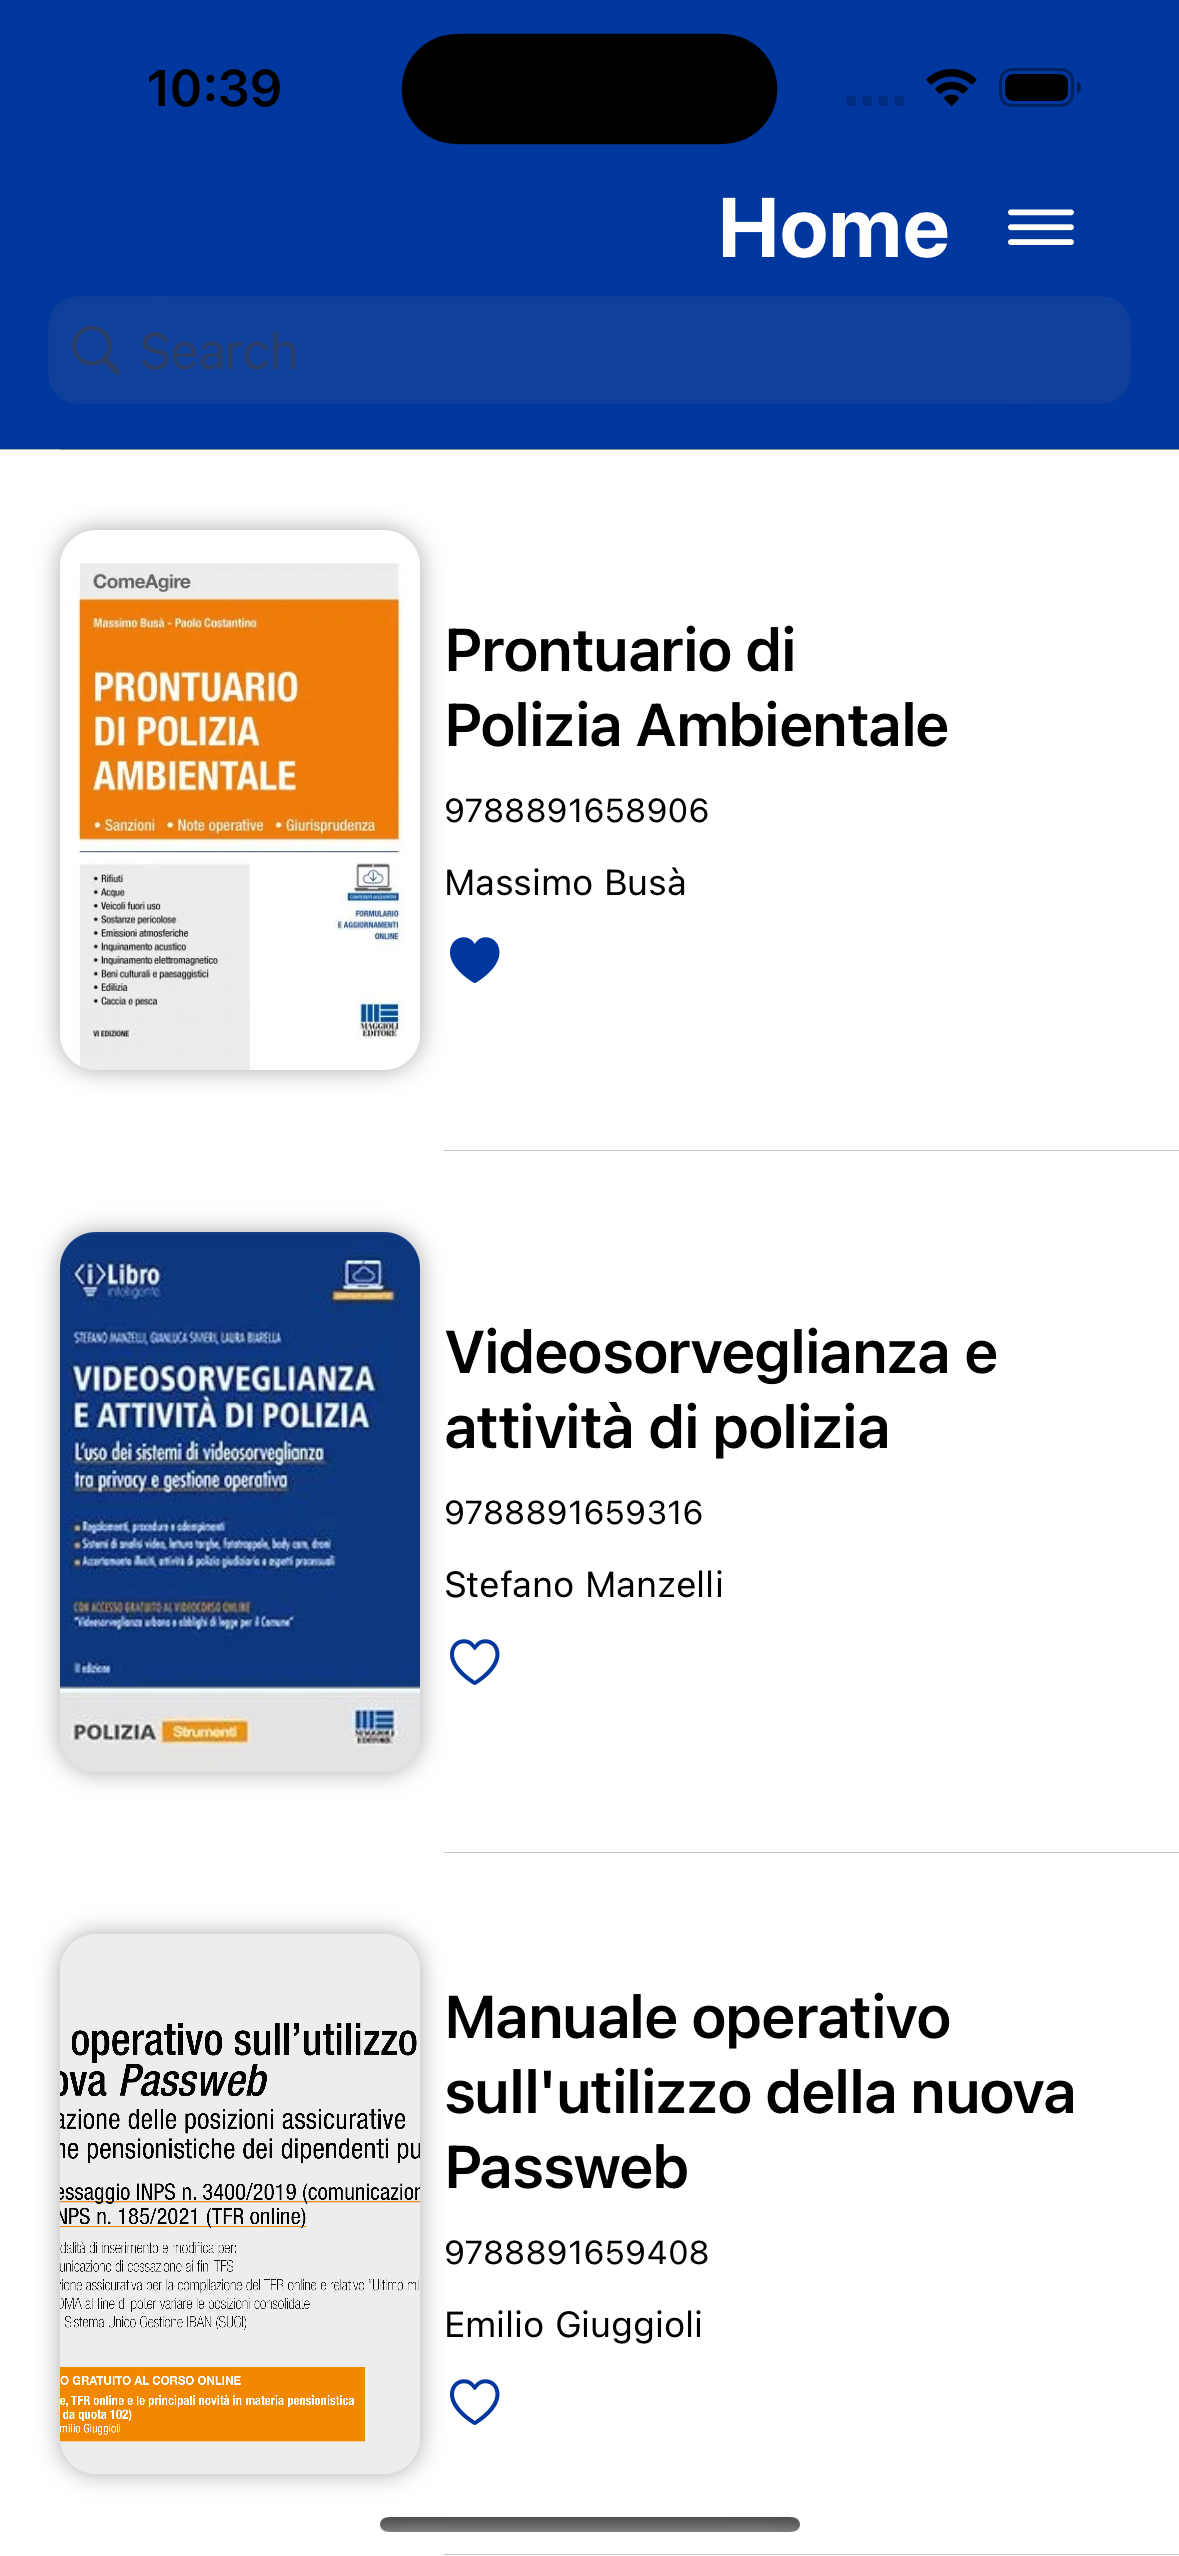
\includegraphics[width=0.26\textwidth]{img/Simulator Screen Shot - iPhone 14 Pro - 2022-10-05 at 10.39.58.png}
        \caption{Schermata home principale}
        \label{home-ios}
    \end{figure}
    
    \begin{figure}[H]
        \centering
        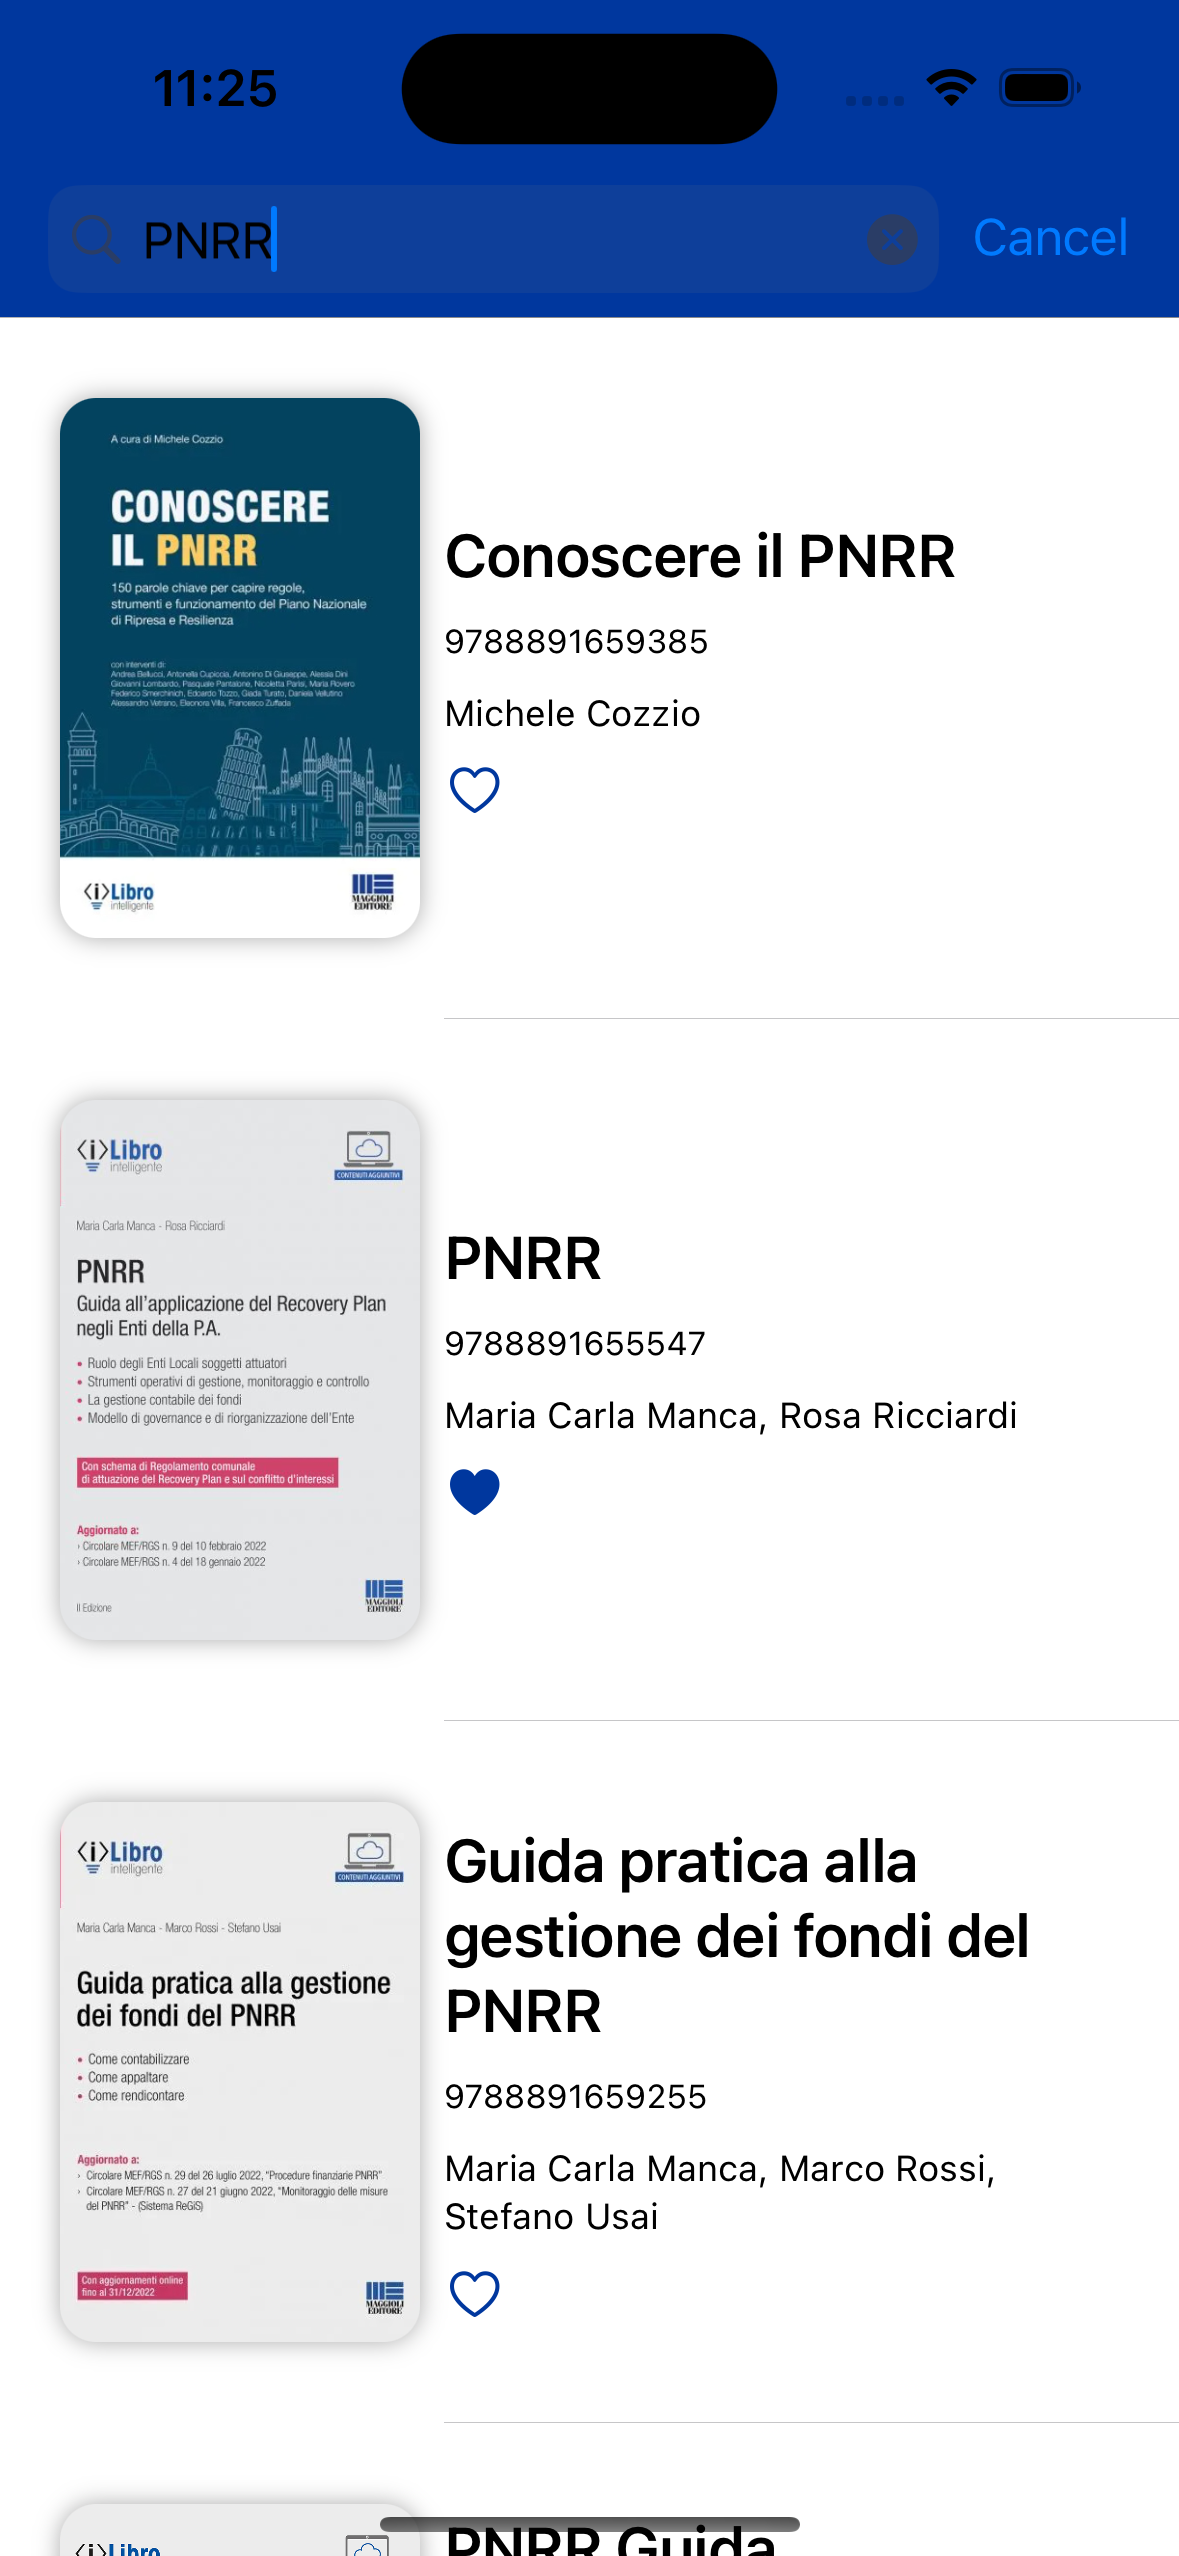
\includegraphics[width=0.26\textwidth]{img/Simulator Screen Shot - iPhone 14 Pro - 2022-10-05 at 11.25.21.png}
        \caption{Esempio di ricerca}
        \label{ricerca-ios}
    \end{figure}

    \begin{figure}[H]
        \centering
        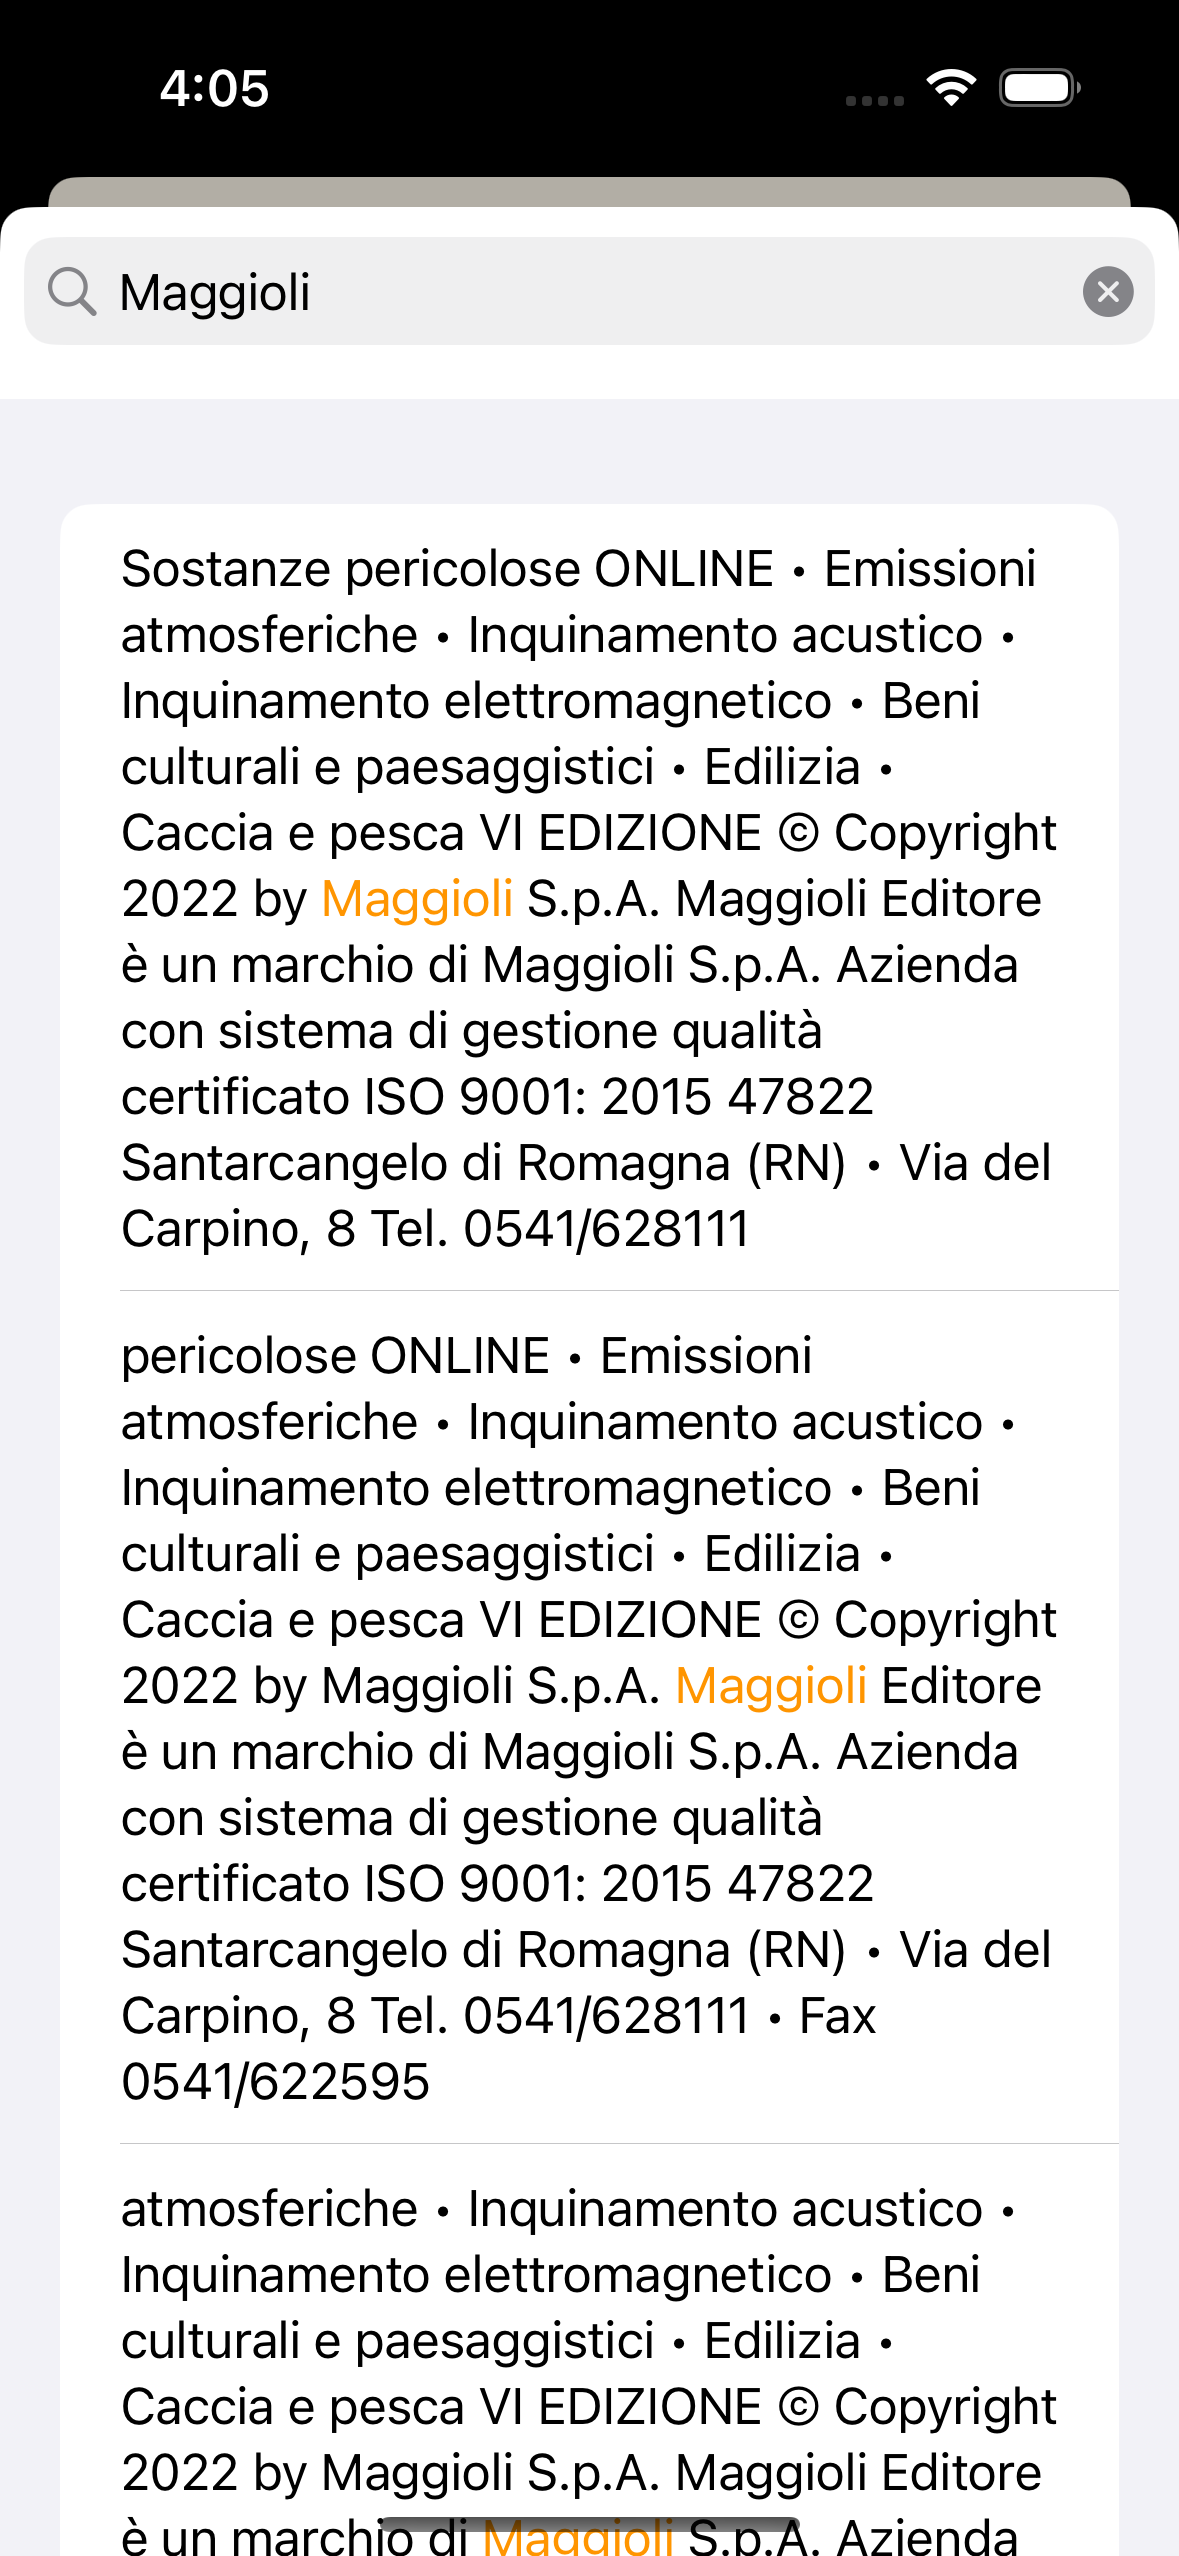
\includegraphics[width=0.26\textwidth]{img/ricerca_testo_ios.png}
        \caption{Ricerca testuale nel contenuto}
        \label{ricerca_testo-ios}
    \end{figure}

    \begin{figure}[H]
        \centering
        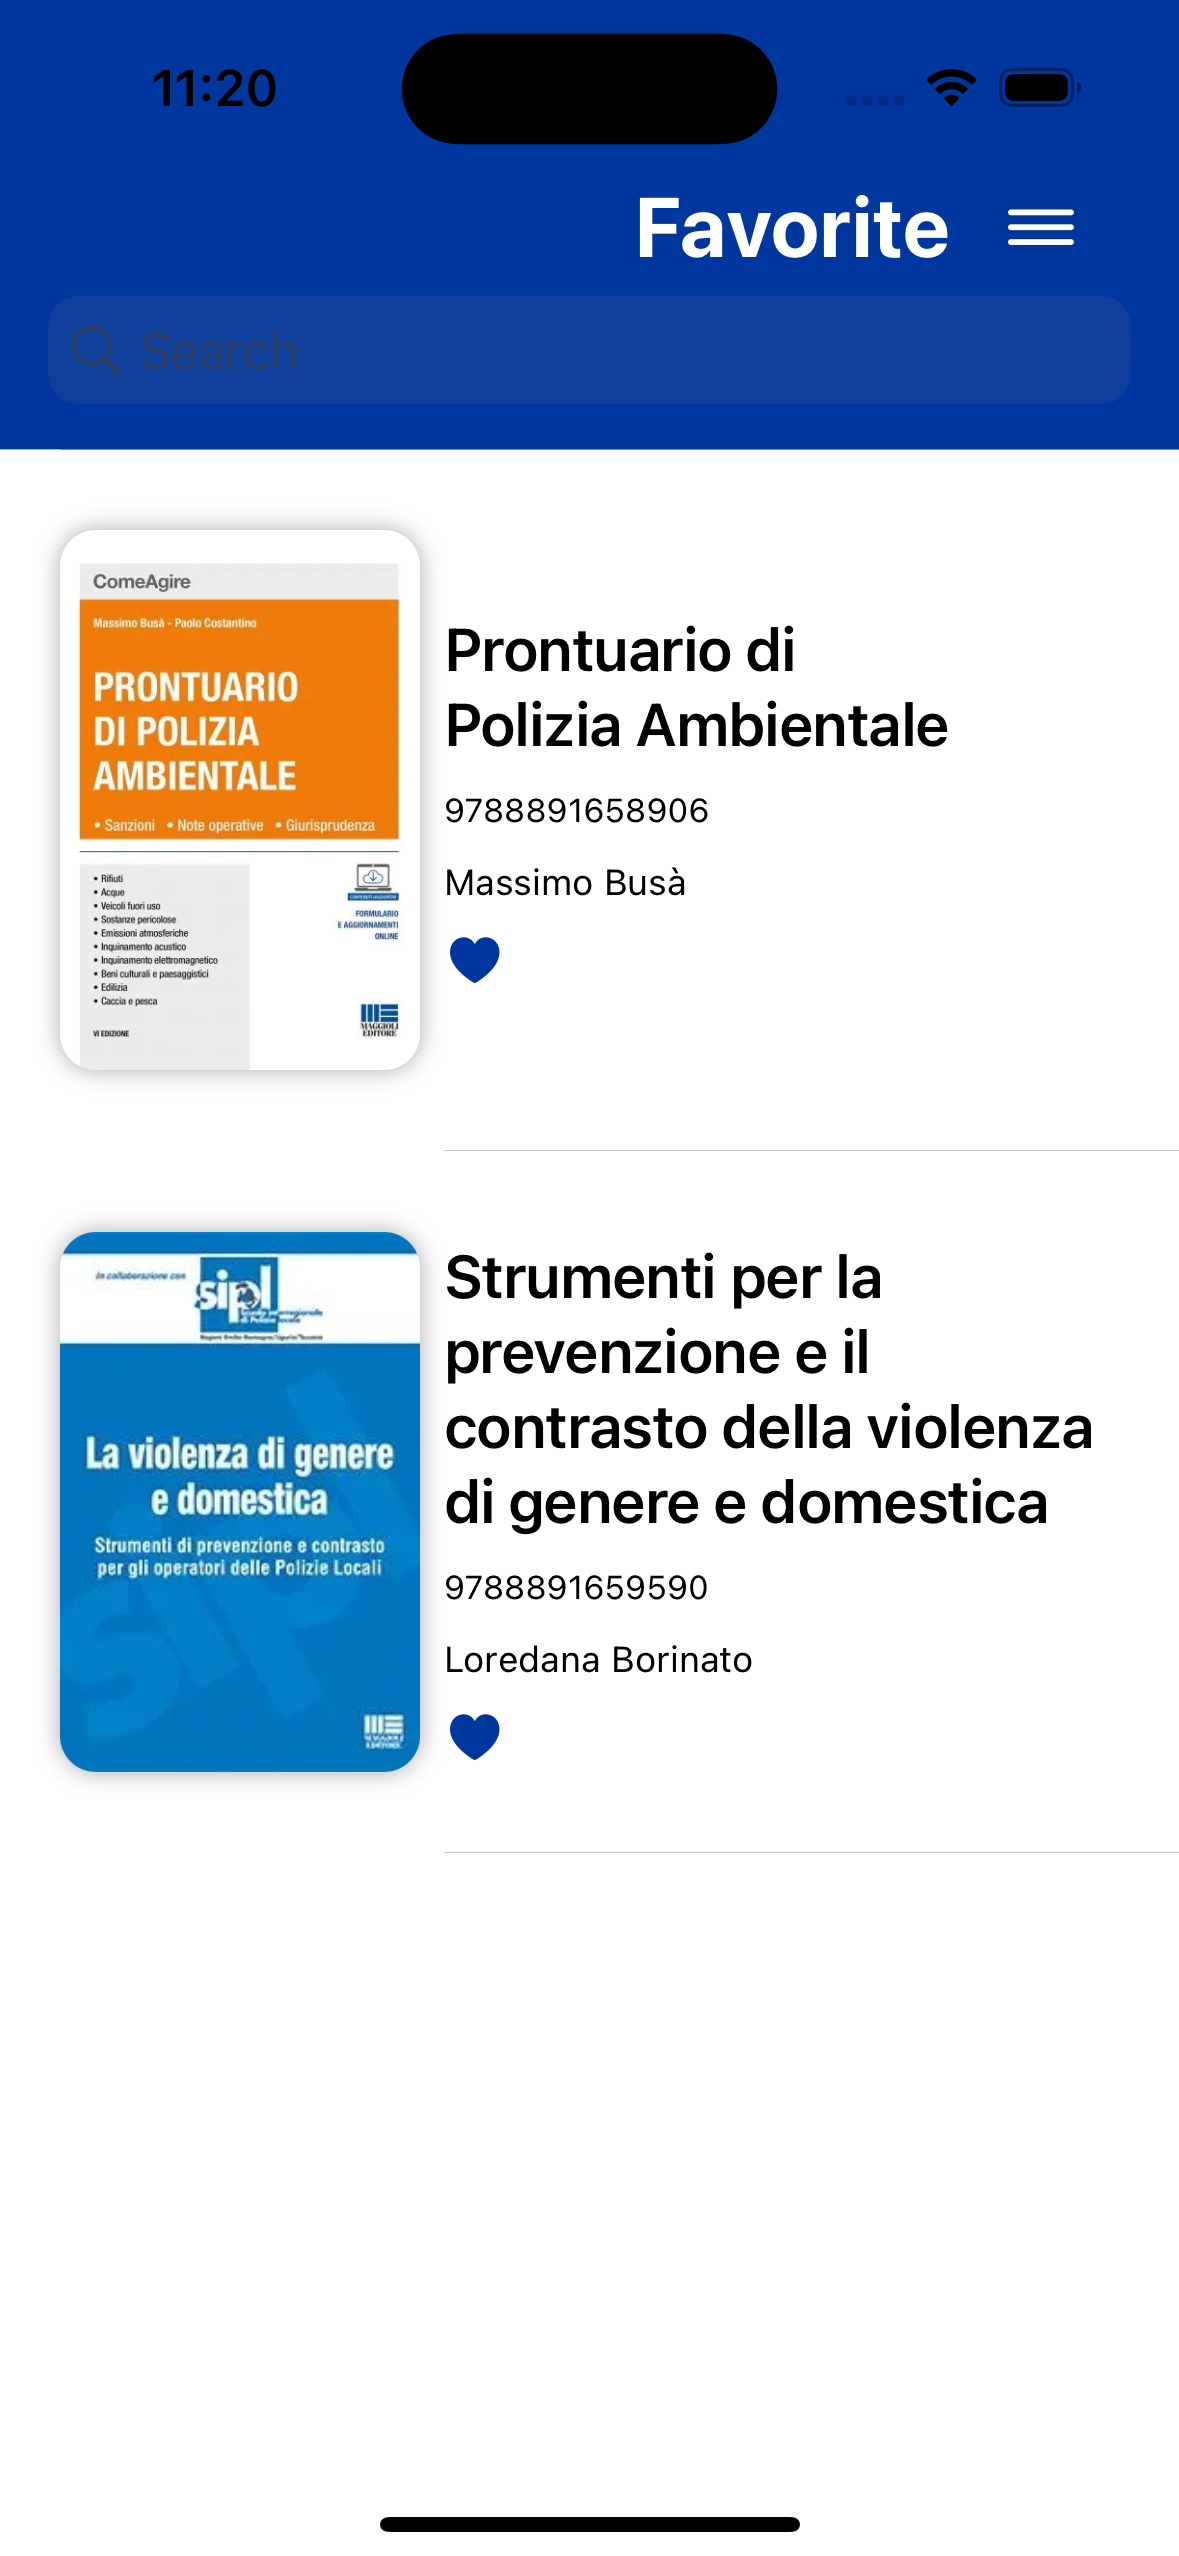
\includegraphics[width=0.26\textwidth]{img/Simulator Screen Shot - iPhone 14 Pro - 2022-10-05 at 11.20.04.png}
        \caption{Schermata dei preferiti}
        \label{preferiti-ios}
    \end{figure}

    \begin{figure}[H]
        \centering
        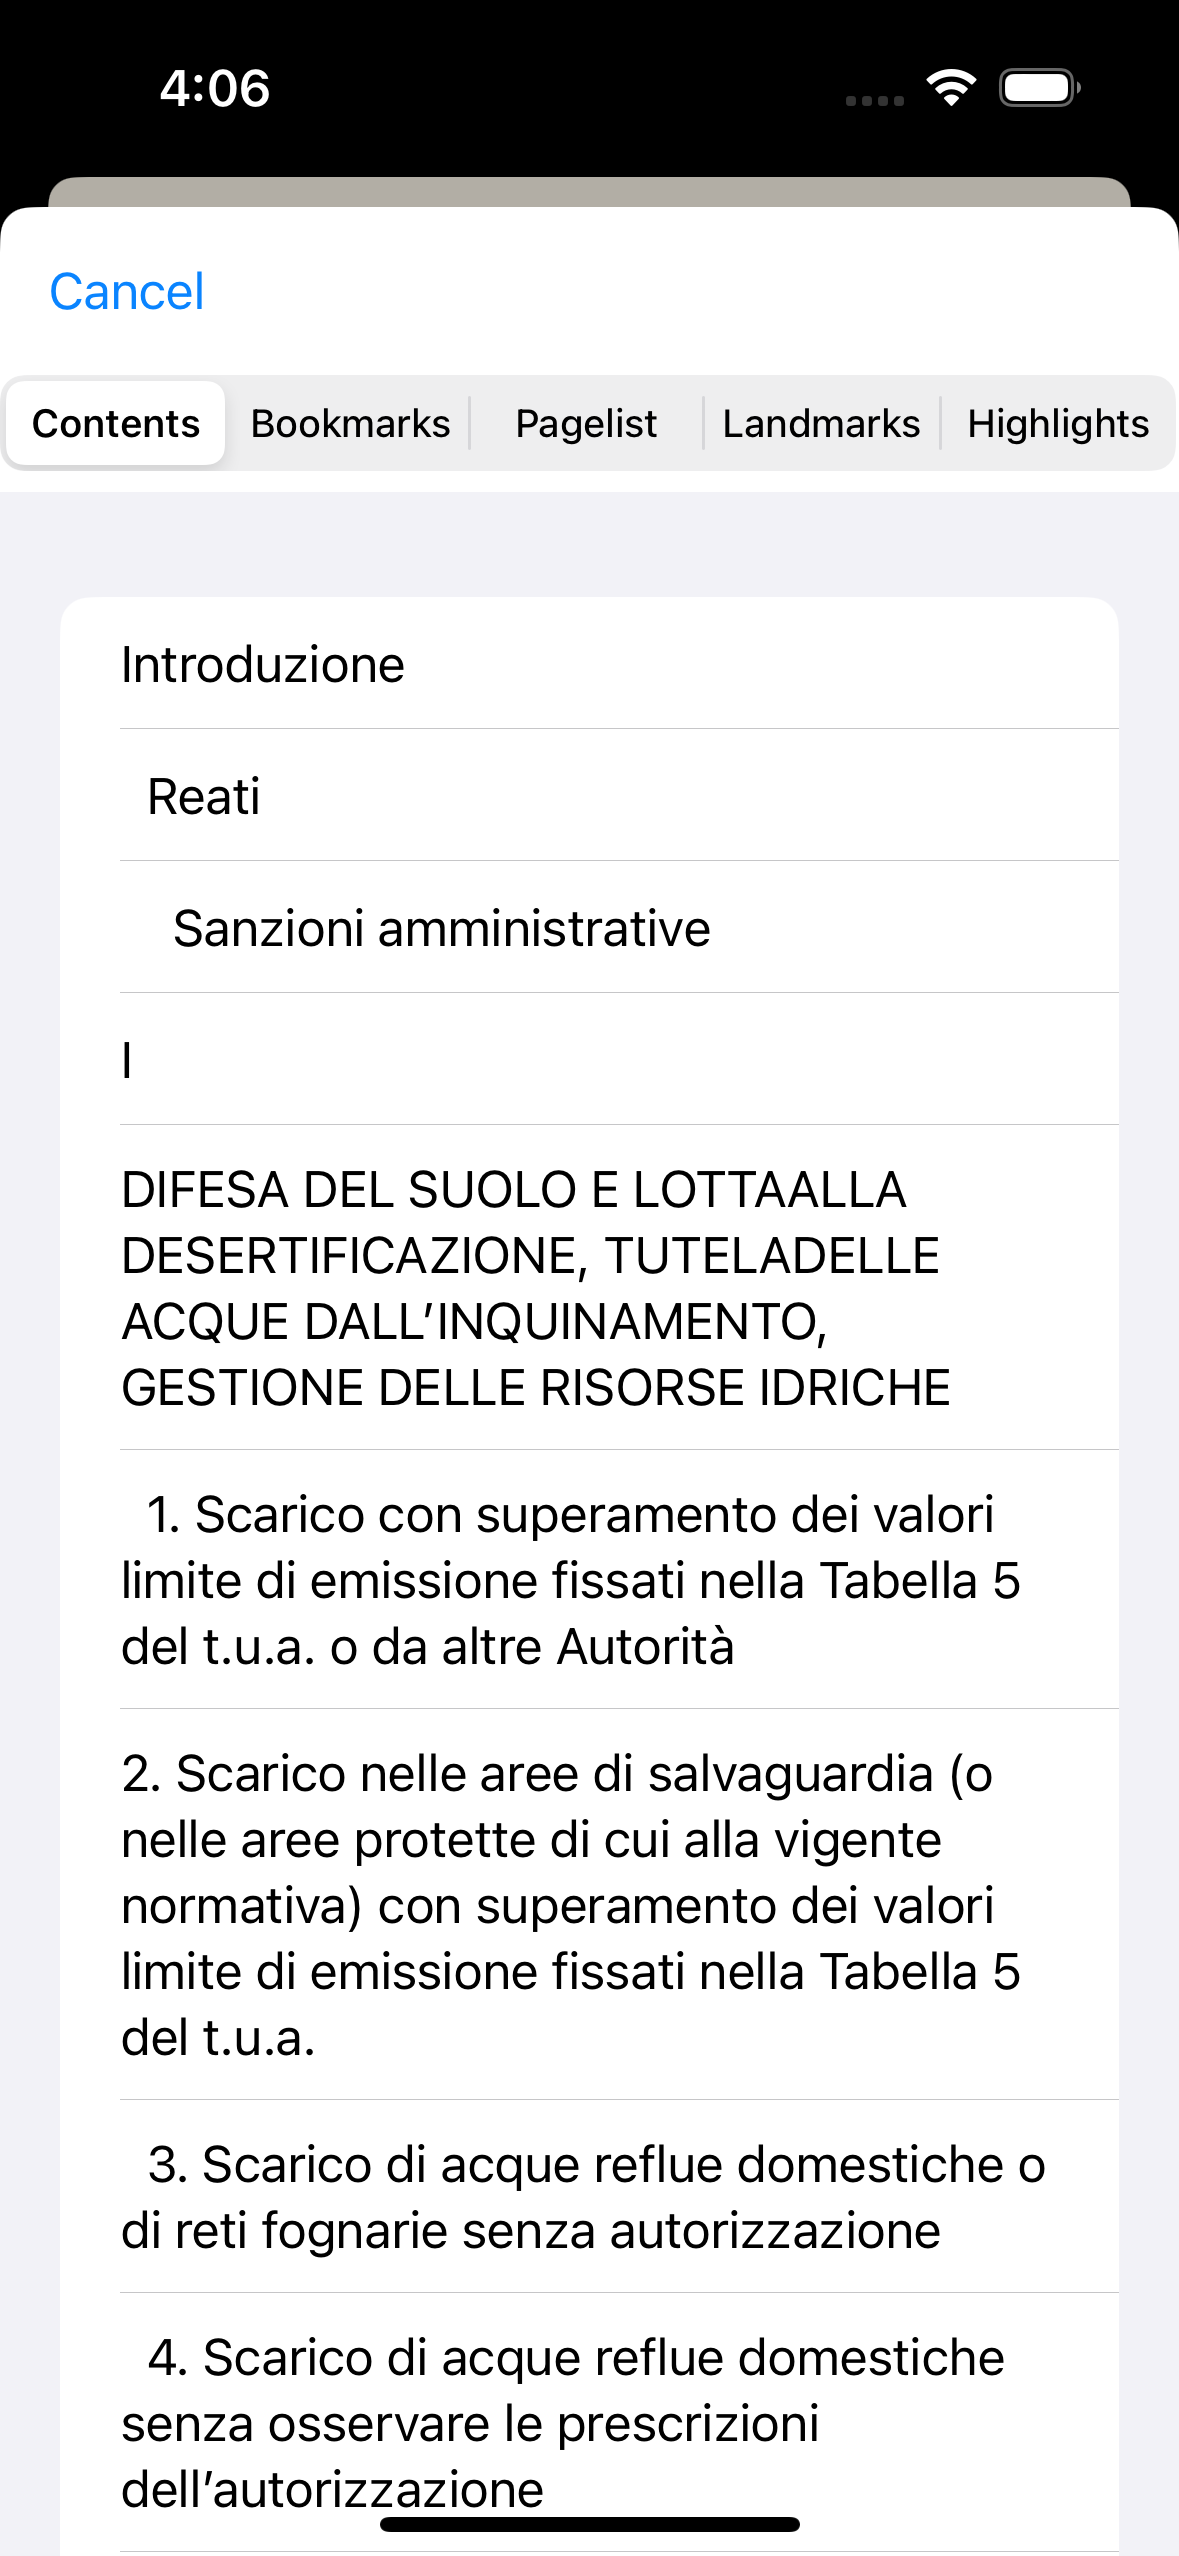
\includegraphics[width=0.26\textwidth]{img/toc_ios.png}
        \caption{Elenco dei contenuti (TOC) del documento}
        \label{toc-ios}
    \end{figure}

    \begin{figure}[H]
        \centering
        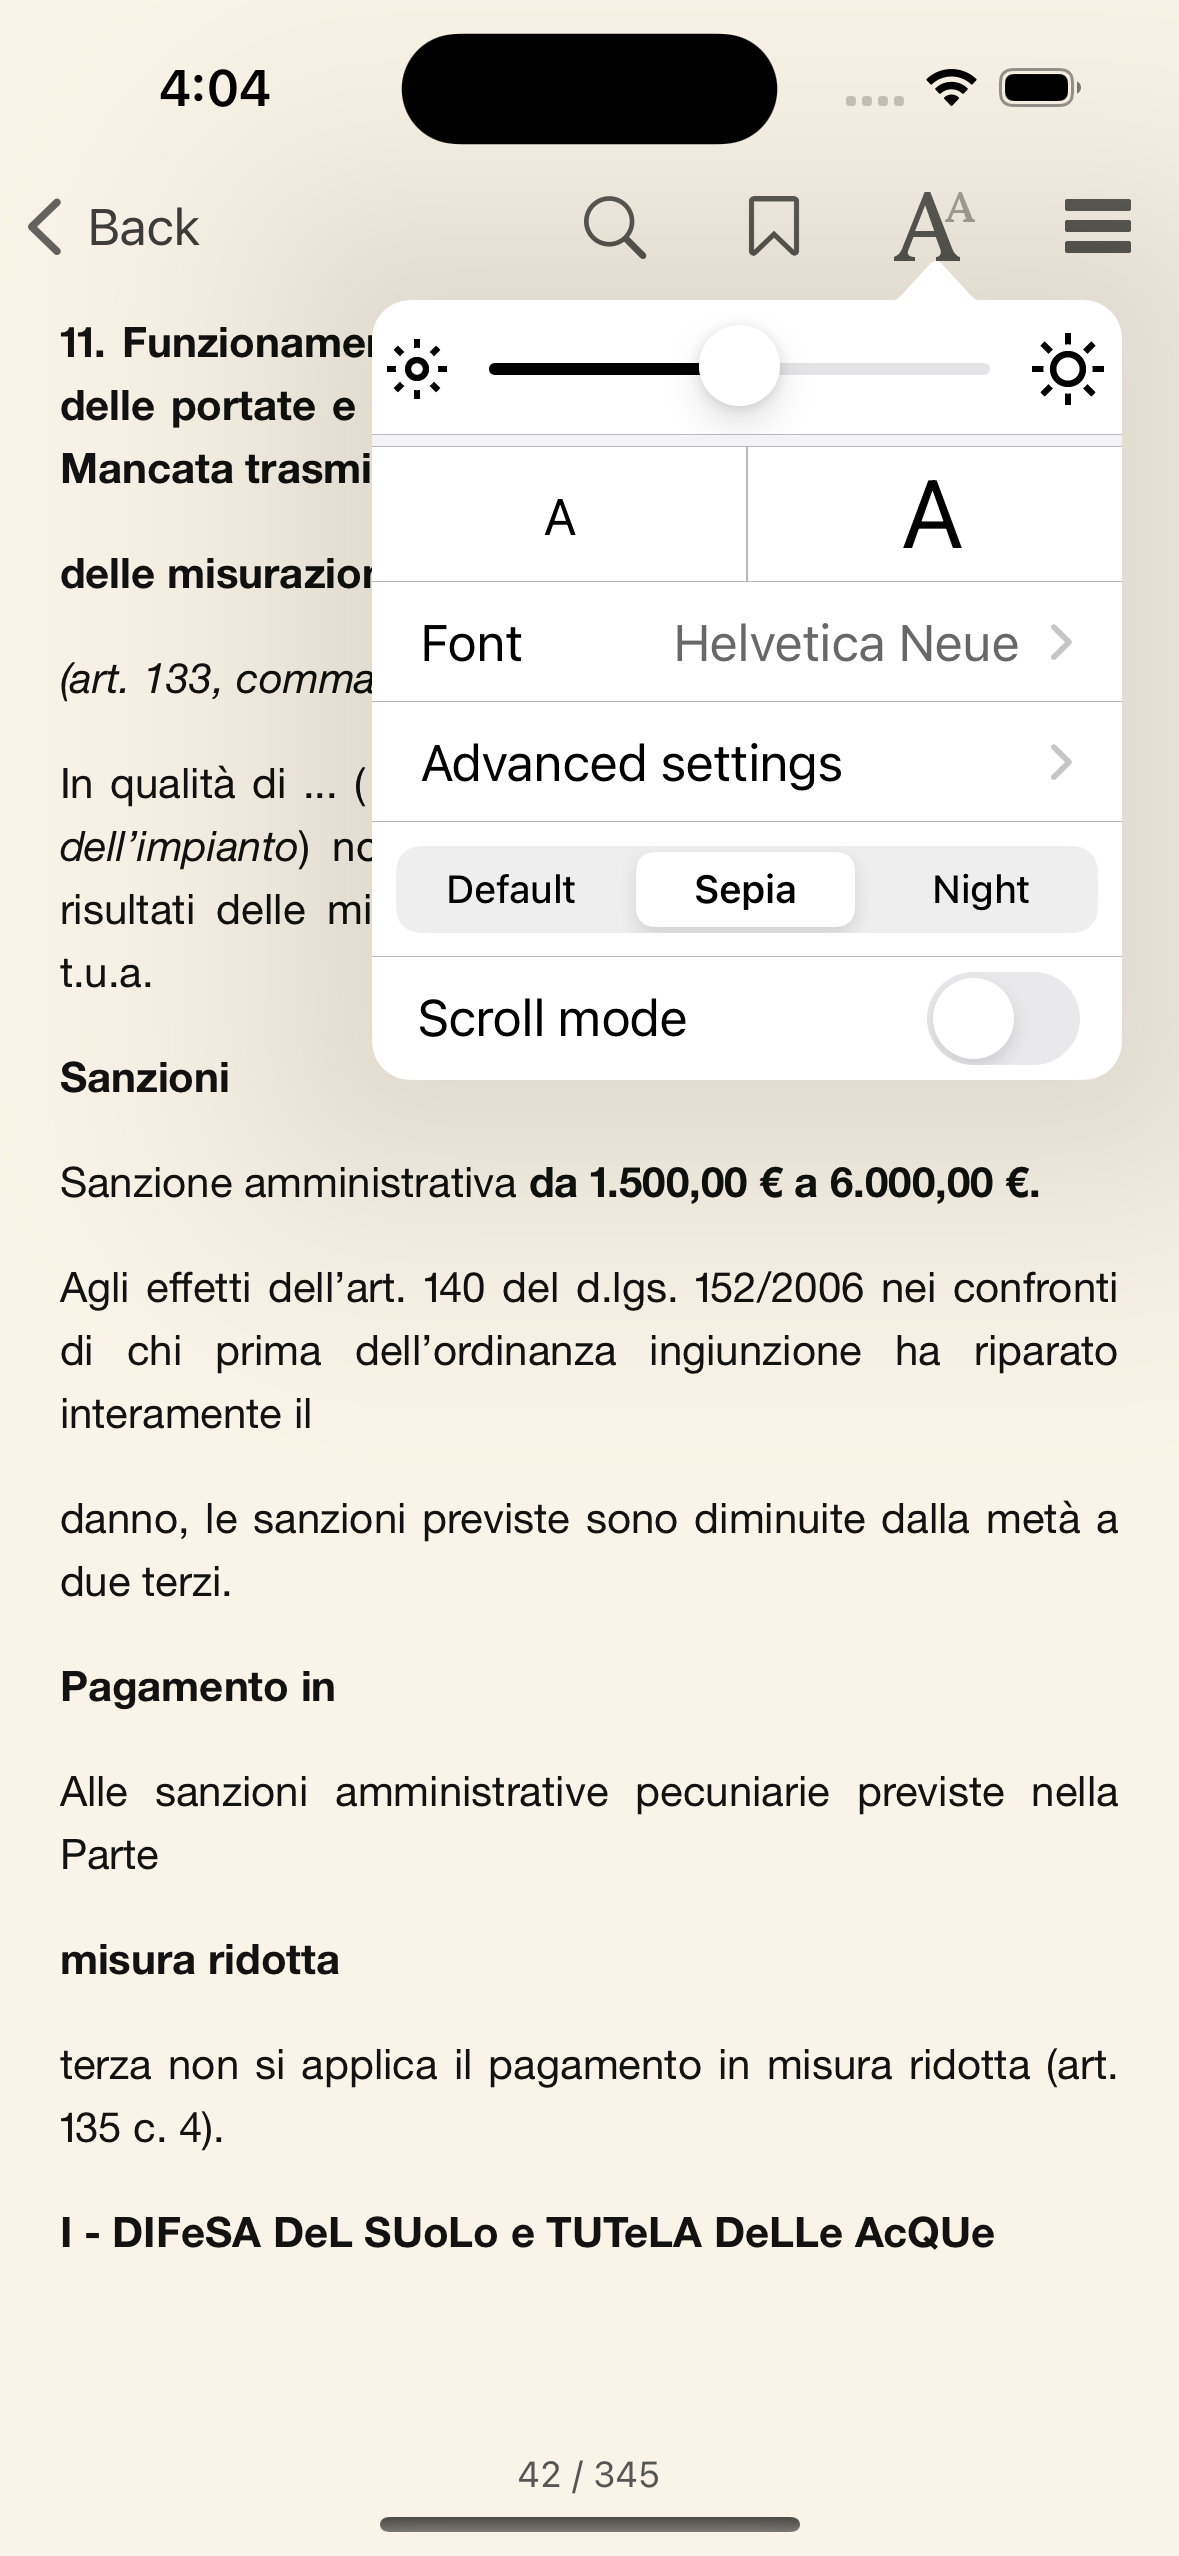
\includegraphics[width=0.26\textwidth]{img/reader_settings_ios.png}
        \caption{Reader}
        \label{readersettings-ios}
    \end{figure}
    
    \begin{figure}[H]
        \centering
        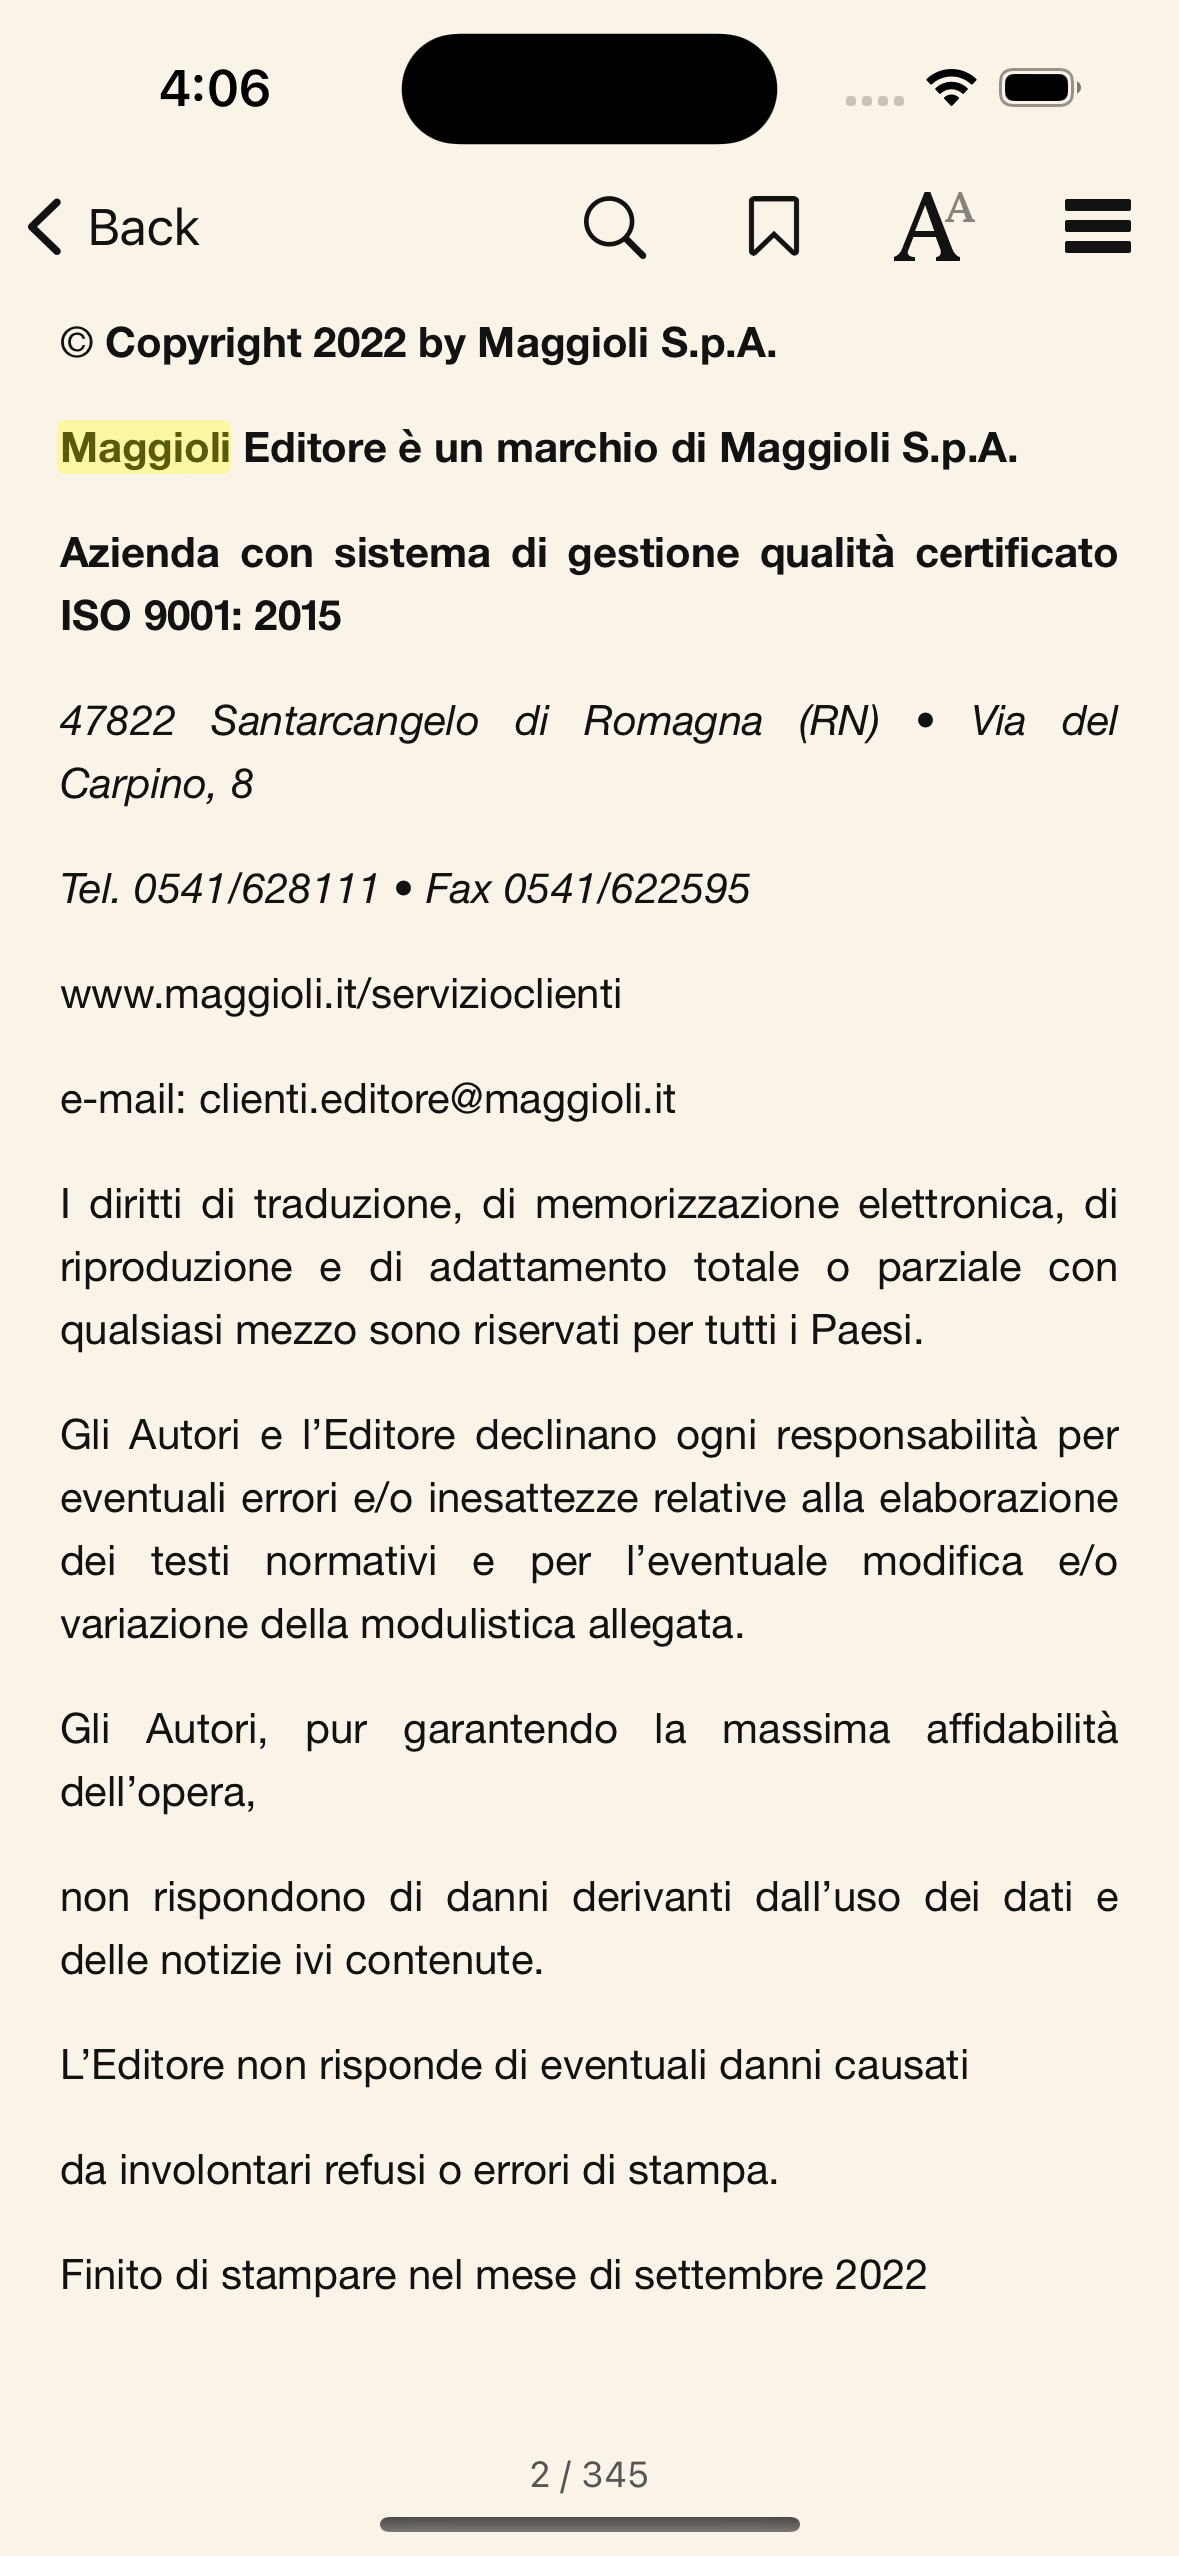
\includegraphics[width=0.26\textwidth]{img/ricerca_testo2_ios.png}
        \caption{Evidenziazioni automatiche delle occorrenze del testo cercato}
        \label{ricerca_testo2-ios}
    \end{figure}
\end{multicols}